%\documentclass[hyperpdf,nobind,draft,oneside]{hepthesis}  %% For normal draft builds, no figs
%\documentclass[hyperpdf,nobind,draft,twoside]{hepthesis}  %% For normal draft builds, no figs
%\documentclass[hyperpdf,nobind,draft,hidefrontback]{hepthesis}  %% For short draft builds
\documentclass[hyperpdf,bindnopdf]{hepthesis}  %%For Cambridge soft-bound version
%\documentclass[hyperpdf,oneside]{hepthesis}  %% For Cambridge hard-bound version

%% Put package includes etc... into a seperate preamble.tex to keep things tidy
\usepackage{xspace}
\usepackage{tikz}
%\usepackage{morefloats,subfig,afterpage}
\usepackage{mathrsfs} % script font
\usepackage{verbatim}
\usepackage{cite}
\usepackage{graphicx}
\usepackage{caption}
\usepackage{subcaption}

%% Load special font packages here if you wish
\usepackage{lmodern}  % lmodern, mathpazo, euler

%% Using Babel allows other languages to be used and mixed-in easily
\usepackage[english]{babel}
\selectlanguage{english}

%% Use the tikz-feynman package for Feynman diagram.
\usepackage[compat=1.1.0]{tikz-feynman}

%% Tweak so maths adapts its boldness to match the context.
\makeatletter
\g@addto@macro\bfseries\boldmath
\makeatother

%% Maths
\usepackage{resources/abmath}
\DeclareRobustCommand{\mymath}[1]{\ensuremath{\maybebmsf{#1}}}
% \DeclareRobustCommand{\parenths}[1]{\mymath{\left({#1}\right)}\xspace}
% \DeclareRobustCommand{\braces}[1]{\mymath{\left\{{#1}\right\}}\xspace}
% \DeclareRobustCommand{\angles}[1]{\mymath{\left\langle{#1}\right\rangle}\xspace}
% \DeclareRobustCommand{\sqbracs}[1]{\mymath{\left[{#1}\right]}\xspace}
% \DeclareRobustCommand{\mods}[1]{\mymath{\left\lvert{#1}\right\rvert}\xspace}
% \DeclareRobustCommand{\modsq}[1]{\mymath{\mods{#1}^2}\xspace}
% \DeclareRobustCommand{\dblmods}[1]{\mymath{\left\lVert{#1}\right\rVert}\xspace}
% \DeclareRobustCommand{\expOf}[1]{\mymath{\exp{\!\parenths{#1}}}\xspace}
% \DeclareRobustCommand{\eexp}[1]{\mymath{e^{#1}}\xspace}
% \DeclareRobustCommand{\plusquad}{\mymath{\oplus}\xspace}
% \DeclareRobustCommand{\logOf}[1]{\mymath{\log\!\parenths{#1}}\xspace}
% \DeclareRobustCommand{\lnOf}[1]{\mymath{\ln\!\parenths{#1}}\xspace}
% \DeclareRobustCommand{\ofOrder}[1]{\mymath{\mathcal{O}\parenths{#1}}\xspace}
% \DeclareRobustCommand{\SOgroup}[1]{\mymath{\mathup{SO}\parenths{#1}}\xspace}
% \DeclareRobustCommand{\SUgroup}[1]{\mymath{\mathup{SU}\parenths{#1}}\xspace}
% \DeclareRobustCommand{\Ugroup}[1]{\mymath{\mathup{U}\parenths{#1}}\xspace}
% \DeclareRobustCommand{\I}[1]{\mymath{\mathrm{i}}\xspace}
% \DeclareRobustCommand{\colvector}[1]{\mymath{\begin{pmatrix}#1\end{pmatrix}}\xspace}
\DeclareRobustCommand{\Rate}{\mymath{\Gamma}\xspace}
\DeclareRobustCommand{\RateOf}[1]{\mymath{\Gamma}\parenths{#1}\xspace}

%% High-energy physics stuff
\usepackage{resources/abhep}
%\usepackage{resources/SIunits}
%\usepackage{hepnames}
%\usepackage{hepunits}

\begin{comment}
TODO: cross-section, nu and nu bar combos, proton, neutron, electron, muon, tau etc
\end{comment}

% Use \xspace at the end of the macros
% Use \text for text of units in macro
% write 5--10 for 5 to 10
% \mathrm{...} macro, i.e. $\mathrm{d}f/\mathrm{d}x$ → df /dx, not $df/dx$ → df /dx
% So put the whole of each mathematical expression in math mode (and drop out of it via \mathrm or \text if needed).
% Negative numbers should be written in math mode
% always wrap text in your equations in the \mathrm macro, which does it right

%% Personal macros
\DeclareRobustCommand{\chips}{\textsc{Chips}\xspace}
\DeclareRobustCommand{\chipsm}{\textsc{Chips-M}\xspace}
\DeclareRobustCommand{\chipsfive}{\textsc{Chips-5}\xspace}
\DeclareRobustCommand{\nova}{NOvA\xspace}
\DeclareRobustCommand{\minos}{\textsc{Minos}\xspace}
\DeclareRobustCommand{\numi}{NuMI\xspace}
\DeclareRobustCommand{\genie}{\textsc{Genie}\xspace}
\DeclareRobustCommand{\root}{\textsc{Root}\xspace}
\DeclareRobustCommand{\tensorflow}{\textsc{Tensorflow}\xspace}
\DeclareRobustCommand{\python}{\textsc{Python}\xspace}
\DeclareRobustCommand{\google}{\textsc{Google}\xspace}

\DeclareRobustCommand{\arXivCode}[1]{arXiv:#1}
\DeclareRobustCommand{\CP}{\ensuremath{\mathcal{CP}}\xspace}
\DeclareRobustCommand{\CPviolation}{\CP-violation\xspace}
\DeclareRobustCommand{\CPv}{\CPviolation}
\DeclareRobustCommand{\LHC}{LHC\xspace}
\DeclareRobustCommand{\CERN}{CERN\xspace}
\DeclareRobustCommand{\bphysics}{\Pbottom-physics\xspace}
\DeclareRobustCommand{\bhadron}{\Pbottom-hadron\xspace}
\DeclareRobustCommand{\Bmeson}{\PB-meson\xspace}
\DeclareRobustCommand{\bbaryon}{\Pbottom-baryon\xspace}
\DeclareRobustCommand{\Bdecay}{\PB-decay\xspace}
\DeclareRobustCommand{\bdecay}{\Pbottom-decay\xspace}
\DeclareRobustCommand{\BToKPi}{\HepProcess{ \PB \to \PK \Ppi }\xspace}
\DeclareRobustCommand{\BToPiPi}{\HepProcess{ \PB \to \Ppi \Ppi }\xspace}
\DeclareRobustCommand{\BToKK}{\HepProcess{ \PB \to \PK \PK }\xspace}
\DeclareRobustCommand{\BToRhoPi}{\HepProcess{ \PB \to \Prho \Ppi }\xspace}
\DeclareRobustCommand{\BToRhoRho}{\HepProcess{ \PB \to \Prho \Prho }\xspace}
\DeclareRobustCommand{\X}{\thesismath{X}\xspace}
\DeclareRobustCommand{\Xbar}{\thesismath{\overline{X}}\xspace}
\DeclareRobustCommand{\Xzero}{\HepGenParticle{X}{}{0}\xspace}
\DeclareRobustCommand{\Xzerobar}{\HepGenAntiParticle{X}{}{0}\xspace}
\DeclareRobustCommand{\epluseminus}{\Ppositron\!\Pelectron\xspace}
\DeclareRobustCommand{\protonproton}{\Pproton\APantiproton\xspace}


%% You can set the line spacing this way
%\setallspacing{double}
%% or a section at a time like this
%\setfrontmatterspacing{double}

%% Define the thesis title and author
\title{Multi-task Convolution Neural Networks for the \chips Experiment}
\author{Josh Chalcraft Tingey}

%% Doc-specific PDF metadata
\makeatletter
\@ifpackageloaded{hyperref}{%
\hypersetup{%
  pdftitle = {Convolution Neural Networks for the CHIPS R&D Project},
  pdfsubject = {Josh Tingey's PhD thesis},
  pdfkeywords = {CHIPS, physics, CNN, Machine Learning},
  pdfauthor = {\textcopyright\ Josh Tingey}
}}{}
\makeatother

%% Start the document
\begin{document}

%% Define the un-numbered front matter
\begin{frontmatter}
  \titlepage[University College London]{ %%%%%%%%%%%%%%%%%%%%%%%%%%%%%%%%%%%%%%%%%%%%%%%%%%%%%%%%%%%
    Submitted to University College London in fulfilment of the \\
    requirements for the award of the degree of Doctor of Philosophy
}

\begin{declaration} %%%%%%%%%%%%%%%%%%%%%%%%%%%%%%%%%%%%%%%%%%%%%%%%%%%%%%%%%%%%%%%%%%%%%%%%%%%%%%
    I, Josh Chalcraft Tingey confirm that the work presented in this thesis is my own. Where
    information has been derived from other sources, I confirm that this has been indicated in the
    thesis.
    \vspace*{1cm}
    \begin{flushright}
        Josh Tingey
    \end{flushright}
\end{declaration}

\begin{abstract} %%%%%%%%%%%%%%%%%%%%%%%%%%%%%%%%%%%%%%%%%%%%%%%%%%%%%%%%%%%%%%%%%%%%%%%%%%%%%%%%%
    %\thispagestyle{empty}
    blah blah blah
\end{abstract}

\begin{acknowledgements} %%%%%%%%%%%%%%%%%%%%%%%%%%%%%%%%%%%%%%%%%%%%%%%%%%%%%%%%%%%%%%%%%%%%%%%%%
    blah blah blah
\end{acknowledgements}

\tableofcontents %%%%%%%%%%%%%%%%%%%%%%%%%%%%%%%%%%%%%%%%%%%%%%%%%%%%%%%%%%%%%%%%%%%%%%%%%%%%%%%%%
\thispagestyle{empty} %% I don't want a page number on the following blank page either. %%%%%%%%%%
\end{frontmatter}

%% Define the main body of the thesis
\begin{mainmatter}
  %\chapter{Common blocks}
\label{chap:common}

%% Restart the numbering to make sure that this is definitely page #1!
\pagenumbering{arabic}

hello ello llo

This .tex file aims to outline how various things should be implemented within the thesis
from references to diagrams the symbols etc\dots

- We use english spelling of everything throughout the thesis

- Write the way that is natural in your head, so you are not contorting your thoughts to fit an unnatural style

- We capitalise just the first word in section, chapter and whole-document titling.

- Don't have unnecessary hyphens for weird phrases, just write it as you would in clear plain english

- Use short sentences most of the time to make work clearer and punchier. More than two lines is probably bad.

- Use the 'english comma' to show how to read the text

- Use non-breaking spaces all over the place ~

- spell out small numbers

- Prefer the default float-spec, [tbp],

- Also read booktabs’ excellent manual on how table formatting should look: in short, never use vertical rules.

- Standard Model is capitalised

- Put all particle in italics (hepnames and hepparticles does this all for you)

\begin{itemize}
    \item \eV
    \item \text{e\kern-0.15ex V}\xspace
    \item \minos
\end{itemize}

\eV

\CC

\text{e\kern-0.15ex V}\xspace

$\int \mathrm{d}x \sin^n{x} \cos^m{x} \quad .$

%% We define many common macros to be used throughout the thesis for various things...
\begin{itemize}
    \item \chips
    \item \nova
    \item \minos
\end{itemize}

%% Quotes if we want to put them in 
\chapterquote{Laws were made to be broken.}%
{Christopher North, 1785--1854}%: Blackwood's Magazine May 1830

Section~\ref{sec:nittygritty} %% refer to sections like this
Table~\ref{tab:a} %% refer to a table like this
Ref.~\cite{xyz} %% if you every refer directly to the reference


${\nu} + p^{+} \rightarrow n + e^{+}$

~\cite{chadwick1914}.


%% The defined macros should always be used
Once upon a time there was \chips which was very nice for \nova which like to use \unit{10}{\GeV} because
of \minos which was very naughty

%% Feynman diagrams
%% You have to use lualatex to get this working
\feynmandiagram [horizontal=a to b] {
i1 [particle=\(e^{-}\)] -- [fermion] a -- [fermion] i2 [particle=\(e^{+}\)],
a -- [photon, edge label=\(\gamma\), momentum'=\(k\)] b,
f1 [particle=\(\mu^{+}\)] -- [fermion] b -- [fermion] f2 [particle=\(\mu^{-}\)],
};

Symmetries, either intact or broken, have proved to be at the heart
of how matter interacts. The Standard Model of fundamental interactions
(SM) is composed of three independent continuous symmetry groups denoted
$\SUgroup{3} \times \SUgroup{2} \times \Ugroup{1}$, representing the
strong force, weak isospin and hypercharge
respectively~\cite{Phys.Rev.Lett.19.1264, Phys.Rev.D2.1285,hep-ph/0410370}.

\section{Neutral meson mixing}
\label{sec:neutralmixing}
We can go a long way with an effective Hamiltonian approach in
canonical single-particle quantum mechanics. To do this we construct
a wavefunction from a combination of a generic neutral meson state
$\ket{\Xzero}$ and its anti-state $\ket{\Xzerobar}$:

\begin{figure}
    \includegraphics[width=\largefigwidth]{diagrams/4-chips/chips_render_1}
    \caption[CKM Fitter constraints on \alphaCKM.]%
    {CKM Fitter constraints on \alphaCKM from combined \BToPiPi,
        \BToRhoPi and \BToRhoRho decay analyses.}
    \label{fig:chips_render_1}
\end{figure}

\begin{sidewaysfigure}
    \begin{center}
        \includegraphics[width=0.8\textheight]{diagrams/4-chips/chips_event}
        \caption[Cross-section view of \LHCb, cut in the non-bending $y$--$z$ plane]%
        {Cross-section view of \LHCb, cut in the non-bending $y$--$z$ plane.}
        \label{fig:chips_event}
    \end{center}
\end{sidewaysfigure}


Since both \bhadron{s} are preferentially produced in the same direction
and are forward-boosted along the beam-pipe, the detector is not required
to have full $4\pi$ solid-angle coverage. \LHCb takes advantage of this
by using a wedge-shaped single-arm detector with angular acceptance
\unit{10-300}{\mrad} in the horizontal (bending) plane~\cite{Amato:1998xt}.

\vspace{1cm}

\begin{center}
    {\hspace{1mm}\Large\vdots\hspace{1cm}}
\end{center}

\vspace{1cm}

The detector is illustrated in \FigureRef{fig:chips_render_1}, showing
the overall scale of the experiment.

%
\begin{equation}
    \ket{\psi(t)} = a(t)\ket{\Xzero} + b(t)\ket{\Xzerobar}
\end{equation}
%
which is governed by a time-dependent matrix differential equation,
%
\begin{equation}
    \I \pdByd{}{t} \colvector{a \\ b}
    =
    \underbrace{%
        \twomatrix{ M_{11}-\frac{\I}{2}\Gamma_{11}
            & M_{12}-\frac{\I}{2}\Gamma_{12} }
        { M_{12}^\ast-\frac{\I}{2}\Gamma_{12}^\ast
            & M_{22}-\frac{\I}{2}\Gamma_{22} }
    }_{\boldmatrix{H}}
    \colvector{a \\ b}
    .
\end{equation}

The single-sided detector design was chosen in preference to a two-armed
design since the detector dimensions are restricted by the layout of the
IP8 (ex-Delphi) cavern in which \LHCb is located. Using all the available
space for a single-arm spectrometer more than compensates in performance
for the \about{50\percent} drop in luminosity.

\section{The \Cerenkov mechanism}
A Huygens construction in terms of spherical shells of probability for photon
emission as the particle progresses along its track shows an effective
``shock-front'' of \Cerenkov emission. This corresponds to an emission cone of
opening angle \thetaCerenkov around the momentum vector for each point on the
track,
%
\begin{subequations}
    \label{eq:cosThetaCk}
    \begin{equation}
        \cos\,\thetaCerenkov  &= \frac{1}{n \beta} +
        \frac{\hbar k}{2p}%
        \parenths{ 1 - \frac{1}{n^2} } \\
        &\,\sim \frac{1}{n \beta}%
        \label{eq:cosThetaCkApprox}
    \end{equation}
\end{subequations}
%
where $\beta \equiv v/c$, the relativistic velocity fraction.

\section{Trigger system}
\label{sec:triggers}
An overview of the \LHCb trigger characteristics broken down by level
is shown in \Table~\ref{tab:TriggerDetails}.

\begin{table}[bp]
    \begin{tabular}{lllll}
                    & L0              & L1              & HLT             \\
        \midrule                                                          \\
        Input rate  & \unit{40}{\MHz} & \unit{1}{\MHz}  & \unit{40}{\kHz} \\
        Output rate & \unit{1}{\MHz}  & \unit{40}{\kHz} & \unit{2}{\kHz}  \\
        Location    & On detector     & Counting room   & Counting room   \\
    \end{tabular}
    \caption{Characteristics of the trigger levels and offline analysis.}
    \label{tab:TriggerDetails}
\end{table}

Here are some funky floats using ``continued captions'', i.e. for a semantically
collected group of float contents which are too numerous to fit into a single
float, such as the pretty circles in the following figure:

\newcommand{\circleimg}[1]{%
    \begin{tikzpicture}
        \draw[color=black,fill=#1,thick] (1,0) circle (1.5cm);
    \end{tikzpicture}%
}

\begin{figure}[hb]
    \subfloat[][Example 1a]{\label{fig:cc1a}\circleimg{red!80}}\quad
    \subfloat[][Example 1b]{\label{fig:cc1b}\circleimg{green!70!yellow}}\quad
    \subfloat[][Example 1c]{\label{fig:cc1c}\circleimg{blue!80}}\quad
    \subfloat[][Example 1d]{\label{fig:cc1d}\circleimg{orange!80!yellow}}
    \caption{Demonstration of \texttt{subfig} continued captions.}
    \label{fig:cc1}
\end{figure}

\begin{figure}[p]
    \ContinuedFloat
    \subfloat[][Example 1e]{\label{fig:cc1e}\circleimg{violet}}\quad
    \subfloat[][Example 1f]{\label{fig:cc1f}\circleimg{cyan}}\quad
    \subfloat[][Example 1g]{\label{fig:cc1g}\circleimg{magenta}}\quad
    \subfloat[][Example 1h]{\label{fig:cc1h}\circleimg{yellow}}
    \caption[]{Demonstration of \texttt{subfig} continued captions (continued).}
\end{figure}

\noindent
This mechanism means that the same float label is used for both pages of
floats. Note that we can refer to \FigureRef{fig:cc1} in general, or to
\FigureRef{fig:cc1g} on \PageRef{fig:cc1g} in particular!

\noindent
Just for the hell of it, let's also refer to \SectionRef{sec:neutralmixing}.

Here are some funky floats using ``continued captions'', i.e. for a semantically
collected group of float contents which are too numerous to fit into a single
float, such as the pretty circles in the following figure

\section{Convolutional Neural Networks}
\label{sec:cnn}

\section{CHIPS Events}
\label{sec:events}

\begin{figure}
    \includegraphics[width=\largefigwidth]{diagrams/4-chips/numi_axis}
    \caption[CKM Fitter constraints on \alphaCKM.]%
    {CKM Fitter constraints on \alphaCKM from combined \BToPiPi,
        \BToRhoPi and \BToRhoRho decay analyses.}
    \label{fig:numi_axis}
\end{figure}

\begin{figure}
    \includegraphics[width=\largefigwidth]{diagrams/4-chips/numi_map}
    \caption[CKM Fitter constraints on \alphaCKM.]%
    {CKM Fitter constraints on \alphaCKM from combined \BToPiPi,
        \BToRhoPi and \BToRhoRho decay analyses.}
    \label{fig:numi_map}
\end{figure}

The expected beam flux at the CHIPS detector location is found from reweighting current

We can use current NuMI beam simulations

Current NuMI beam experiments


Once upon a time there was \chips which was very nice for \nova which like to use \unit{10}{\GeV}

  \chapter{Introduction}
\label{chap:introduction}

%% Restart the numbering to make sure that this is definitely page #1!
\pagenumbering{arabic}

blah blah blah

  \chapter{Neutrino oscillations: theoretical background and current status}
\label{chap:theory}

Consider a simple two body decay
Neutrino physics covers the widest possible range of
Proposal of a mysterious undetector particle to explain beta decays in the 1930s through to the resolutions of a 30-year problem with the confirmation of oscillations in the early 2000s and onto the precision era.
Neutrino oscillations first discoveed in 1957 when Bruno Pornecorvo proposed a model in which neutrinos oscilate to antineutrinos and back, similar to the kain. It was actually shown that neutrinos iscilate from one flavour to another.
The field of neutrino physics is ever expanding with a new generation of experiments planned for the coming years.
This chapter aims to provide an introduction to neutrino

\section{A history of neutrino oscillations}
\label{sec:theoryhistory}

\begin{comment}
TODO: Maybe add a few diagrams of the key plots throughout history
\end{comment}

In the early 20th century, beta decays were assumed to follow the simple two-body process, $A \rightarrow B + e$, where a
nuclei spontaneously an electron, and only an electron. To conserve both energy and angular momentum the ejected electron
must have a discrete kinetic energy defined by the difference in binding energies between the initial and final nuclei.
However, in 1914, J. Chadwick instead measured a continuous energy spectrum for the electron ~\cite{chadwick1914},
placing this theory in doubt.

W. Pauli finally proposed a 'desperate solution' to this paradox in 1930 ~\cite{pauli1930}. If a light, neutrally charged,
spin $1/2$ particle was also produced in the interaction, the continuous energy distribution could be explained. Initially
this mysterious new particle was named the 'neutron'. But, to avoid confusion with the heavy baryon of the same name discovered
in 1932, E. Fermi renamed it the 'neutrino' when he formalised beta decay in 1934 ~\cite{fermi1934}.

The following month, H. Bethe and R. Peierls used Fermi's work to estimate the cross-section of the inverse beta decay process
${\nu} + p^{+} \rightarrow n + e^{+}$ ~\cite{bethe1934}. They calculated a value of less than the very small $10^{-44} cm^2$
and declared 'there is no practically possible way of observing the neutrino.' Although extensive neutrino detection has
proved possible, it hinted at the huge difficulties experimentalists would face hunting down the neutrino and measuring
it's properties in the years to come.

After an initial tentative identification if 1953, F. Reines and C. Cowan made the first confirmed observation of the neutrino
in 1956 ~\cite{cowan1956}. Electron antineutrinos produced in the Savannah River Plan nuclear reactor were detected via the
inverse decay process outlined in the previous paragraph. A 'club-sandwich' detector of three 1500 litre liquid scintillator tanks
and two 200 litre cadmium doped water target tanks, was constructed in an underground room of the reactor building. A total of
330 photomultiplier tubes were then able to measure the prompt positron annihilation signal followed by the gamma ray burst from
the neutron capture in cadmium, the signature identification for the interaction.


Brookhaven two kinds of neutrinos in Ref.~\cite{danby1962}
- Muon neutrino discovered by the 'long track' from the decays of pions from a reactor in 1988, got a nobel prize.
- In 1962 at the alternating gradient synchrotron at Brookhaven, neutrinos created from pion decays together with muons were observed t produce only muons not electrons, this then confirmed the existence of the muon neutrino.
- Neutrinos originating from pion decays primary produce muons, not electron. Detected as single long tracks in a spark chamber.
- Got the 1988 nobel prize for this discovery of the second neutrino.
- Distinct from the previously known electron neutrino
- The neutrinos produced by the pions decay from a accelerator beam, were not the same as the neutrinos observed in beta decay
- Did so by observing that it was far more likely that the neutrinos pro-duced in the decay of pions would interact to create muons, as opposed to electron
- First experiment to construct and use an artificial neutrino beam
%- νμ+p+→μ++n and ̄νμ+p+→e++n with a single neutrino would be expected to happen at the same rate, only muons were produced.
- 34 identified muon events in total no electrons.


Discovery of the tau lepton ~\cite{perl1975}
Also precise z-resonance measurement at lep in the 1990's ~\cite{electroweak2006}
Finally measured by DONUT in 2000 ~\cite{Kodama2001}
- evidence for the third neutrino, finally discovered at DONUT in 2000
- After the discovery of the tau lepton in 1975 ~\cite{perl1975}, this suggested the existence of the third neutrino which DONUT found in 2000.
- DONUT finally found the tau neutrino in 2000 using 800GeV protons from the Tevatron.
- In 2000 the DONUT experiment at the tevatron collider in fermilab performned a direct detection of the tau neutrino completing the three flavour picture.
- Experiments at the LEP e+e- collider in the 1990s made precision measurmnets of the z decay width, from a fir to the data in showed there are exactly three active generations of neutrinos.
- This indicates the number of active neutrino states can only be 1.984+-0.008. Therefore, any as yet undiscovered neutrinos must be sterile, in that they do not couple to the weak interaction.
%- Hence, all flavours of neutrino had been found, but the strongest constraint is due to the width of the Z^0 resonance. 


Homestake deficit observation in Ref.~\cite{davis1968}
first SSU predictions used to compare against homestake in Ref.~\cite{bahcall1968}
Kamiokande II deficit in Ref.~\cite{hirata1989}
SAGE experiment deficit in Ref.~\cite{abazov1991}
GALLEX experiment deficit in Ref.~\cite{anselmann1994}
SSM Prediction for Ga in Ref.~\cite{bahcall1988}
- As the standard model of particle physics was developed, neutrinos were presumed to be massless and occur only in the three flavour eigenstates.
- Various hints that this was not the case kept appearing, leading to neutrino oscillations, by witch one neutrino can oscillate to another flavour and the non-zero masses that follow as a direct consiquence from this.
- In the solar neutrino sector there is the "solar anomaly" noting a deficit of electron neutrino compared to predications made by the standard solar model (SSM)
- First observed at the Homestack experiment, neutrinos ineracted with the chlorine creating radioactive argon atoms, beause it is a noble gas it does not bing to the perchloroethylene and it can be extracted by purging the liquid with gaseous helium and then extracted from the helium with a cooled carbon trap.
- Gallium was also used by other experiments and kamiokande also observed the deficit.
- Also the fluxes measured where not consistent, depending on the energy range probed. Hinting at oscillations dependent on energy,
%- 4p+ 2e−→4He + 2νe+ 26.73MeV−Eν pp-chain in the sun whereEνis the energy of the two neutrinos, and (26.73 MeV -Eν) is the energyemitted as photons
%- νe+37Cl→37Ar +e−(threshold 814 keV) in homestake, periodically flushed with helium
- 400 000 litresof perchloroethylene (a dry-cleaning fluid), containing520 tof chlorine, placed in the Homestake Mine,1.5 kmunderground [24].
%- chlorine solution capable of neutrino capture(νe+37Cl→37Ar + e−).  The atoms of argon were counted and used as a measure of the neutrinoflux.
- he reported experimental rate was about two thirds less than what was expected from theStandard Solar Model (SSM). This large discrepancy, known as thesolar  neutrino  problem, wasinitially believed to be an experimental flaw.
% ν+Ga71→Ge71+e− for sage and gallex
- This is where the future DUNE detector will be housed, nice full circle
- This is in the solar sector

SNO oscillation measurement in Ref.~\cite{ahmad2002}
- neutrino oscillations were one way of explaining this deficit if some of the electron neutrinos converted flavour in flight.
- SNO finally answered the question when it was able to measure three channels with different relation between te flyx or electron neutrinos and the other neutrinos. SNO could prove that the electron neutrinos are changing flavour. WHile the total flux of all neutrinos remains constant and in agrrement with the SSM.
- 1kton tank of heavy (D2O deuterium) water, able to detect three different channels of neutrino interaction
%- νe+d→p+p+e− νx+d→p+n+νx νx+e−→νx+e−
- Cherenkov experiment, with 9500 8inch photomultiplier tubes detectro the light from neutrino interactions.
- Since each of the rates for the three channels has a different relation between the flux of electron neutrinos and the others, SNO could confirm electron neutrinos are changing flavour, with the total flux being constant and in agreement with the SSM.
- electron neutrino CC, NC and elastic scattering also.
- total rate was consistent but less electron neutrinos than expected as they had oscillated.
- However, only electron neutrinos canundergo CC interactions, as solar neutrinos do not have enough energy to produce muonor tau leptons.
- %e+d→p+p+e−(CC) νx+d→p+n+νx(NC) νx+e−→νx+e−(ES) The CC channel is sensitive exclusively to electron neutrinos, whilst the other two are acces-sible by neutrinos of any flavour. 

Atmospheric kamiokande deficit in Ref.~\cite{hirata1988}
IMD detector atmospheric deficit in Ref.~\cite{becker1992}
Superkamiokande direction atmospheric neutrinos in Ref.~\cite{becker1992}
- This is in the atmospheric sector

\section{Neutrino oscillation theory}
\label{sec:theorytheory}

blah blah blah

\section{Current status and the future}
\label{sec:theorystatus}

\subsection{Atmospheric}

\subsection{Accelerator experiments}

\subsection{Reactor experiments}

\subsection{The future}


blah blah blah
  \chapter{The \chips R\&D Project} %%%%%%%%%%%%%%%%%%%%%%%%%%%%%%%%%%%%%%%%%%%%%%%%%%%%%%%%%%%%%%%%
\label{chap:chips}

In pursuit of answers to the open questions outlined in the previous chapter, neutrino experiments
are becoming increasingly, and possibly prohibitively, expensive and impractical. This is
particularly true of the next generation long baseline experiments (DUNE and Hyper-Kamiokande),
with cost estimates reaching billions of dollars and construction times of more than half a
decade. It is also telling that only two future projects receive the vast majority of global
research effort, such is their complexity, cost, and lead time.

It is clear that for detectors to remain practical and affordable into the future, a novel
approach to neutrino detector design is required. This is particularly true is megaton scale
detectors are ever to become a reality. While instrumentation will continue to improve with time,
the statistics of low event counts will always limit neutrino experiments until vastly larger
detectors can be built. Therefore, R\&D efforts must focus on such detectors while attempting to
complement the current and upcoming generation of experiments.

The \chips R\&D project~\cite{adamson2013} aims to develop novel strategies and technologies for
very large yet `cheap as chips' water Cherenkov detectors. Primarily aimed for deployment in long
baseline accelerator scenarios, \chips aims to lower the construction cost per kt of fiducial mass
to between \$200k-\$300k. For comparison, the Super-Kamiokande detector cost approximately \$4
million/kt to build. As physics sensitivity depends on more than just fiducial volume, this
comparison is not entirely rigorous; however, it highlights the scale of cost savings possible.

The \chips concept is to construct cylindrical water Cherenkov detectors that can then be sunk to
the bottom of deep bodies of water on the Earth's surface, such as lakes, reservoirs and flooded
mine pits. The water above the detectors provides a modest overburden from cosmic rays, while the
surrounding water provides support for a lightweight detector structure. By removing the need for
underground excavation and expensive structural support, the cost of construction can be
dramatically reduced.

Additionally, the common practice of building bespoke components for the majority of the detector
is replaced with using modern commercially available components wherever possible. The number of
expensive components, such as photomultiplier tubes is also reduced by only considering
accelerator beam neutrino events, such that full detector instrumentation is not required.

Furthermore, \chips detectors are not only designed to be cheap but practical. Easy to build,
quick to deploy, and upgradable one operational, multiple detector modules can be flexibly
combined depending on available resources. Compared to DUNE and Hyper-Kamiokande that require a
large upfront budget and years to construct, \chips detector modules can be flexibly deployed in
under a year.

\subsubsection*{R\&D effort} %%%%%%%%%%%%%%%%%%%%%%%%%%%%%%%%%%%%%%%%%%%%%%%%%%%%%%%%%%%%%%%%%%%%%

The \chips project consists of multiple R\&D streams outlined below, each with the primary goal of
proving a key component of the \chips concept is viable.

\begin{itemize}
    \item \textbf{Detector construction:} Detailed in Section.~\ref{sec:chips_detector} this
          stream aims to prove that construction and deployment of a \chips detector is possible.
          Two prototype detectors have so far been deployed. Firstly, the very small \chipsm
          detector~\cite{perch2015, pfutznerProto2017, pfutzner2017} deployed into a flooded mine
          pit in northern Minnesota in the summer of 2014. Additionally, the much larger 5kt,
          \chipsfive detector deployed into the same pit in the summer of 2019.

    \item \textbf{Water filtration:} This stream aims to prove that adequate water purity can be
          achieved using cheap, commercially available filtration. Extensive
          studies~\cite{amat2017, campbell2020} have proven that by filtering water directly from
          the flooded mine pit using cheap filtration an adequate attenuation length of greater
          than \unit{50}{\mathrm{m}} is possible. This is not discussed further in this work.

    \item \textbf{Detector sensitivity:} This stream aims to prove that \chips detectors can
          provide significant physics contributions alongside the current and next generation of
          experiments. Single detectors in the NuMI beam and multiple detectors in the future LBNF
          beam have been considered in multiple studies~\cite{pfutzner2017, adde2016, lang2015}.
          This is not discussed further in this work.

    \item \textbf{Data acquisition:} Outlined in Chapter.~\ref{chap:daq} this stream aims to prove
          that a cheap data acquisition system using commercially available components in
          viable~\cite{eijk2018}. \chips implements a novel use of cheap single-board computers to
          collect data from multiple PMTs.

    \item \textbf{Event reconstruction and identification:} Detailed in Chapter.~\ref{chap:cvn}
          this stream aims to prove that modern machine learning techniques can be applied to
          water Cherenkov detectors such as \chips. This work both feeds into the detector
          sensitivity work mentioned above and also allows to detector optimisation studies to be
          carried out.
\end{itemize}

\begin{figure} % CHIPS-M DIAGRAM %
    \includegraphics[width=0.6\textwidth]{diagrams/4-chips/chips_m.png}
    \caption[Picture of the \chipsm detector.]
    {Picture of the \chipsm detector just before deployment. The umbilical cord, carrying cables
        and water pipes is visible, attached to the bottom of the detector.}
    \label{fig:chips_m}
\end{figure}

So far, \chips efforts have been based in the USA to exploit the NuMI beam before the end of its
lifetime. Future plans are focused on the scaling of \chips detectors and the deployment of
multiple modules in the LBNF beam once it becomes operational.

\subsection{The neutrino beam} %%%%%%%%%%%%%%%%%%%%%%%%%%%%%%%%%%%%%%%%%%%%%%%%%%%%%%%%%%%%%%%%%%%
\label{sec:chips_concept_beam} %%%%%%%%%%%%%%%%%%%%%%%%%%%%%%%%%%%%%%%%%%%%%%%%%%%%%%%%%%%%%%%%%%%

- CHIPS will use a neutrino beam to measure,
- These can be measured using four data sample, two for neutrino and two for antineutrinos.
- These sample are produced by "Forward Horn current" FHC and "Reverse Horn current" RHC,
producing predominetetly neutrinos and anti-neutrinos respectively.
- Neutrino oscillation probabilities can then be inferred by comparisons of the observed neutrino
spectra and the near and far detectors.
- Primarily muon neutrinos can be produced by using a particle accelerator to direct a proton beam
at a target. By focusing the pions and kaons this produces, a neutrino beam created from the
downstream decays, creates the muon neutrino beam.
- Better to think of \chips applying to any Beam
- Here we will talk about the NuMI beam as the prime example as that is the one used for the
current generation of \chips prototype.
- Possible future \chips in LBNF which is primarily being built for DUNE
- The \numi beam big paper~\cite{adamson2016}
- How will LBNF be different from NuMI, upgrades etc...

\begin{figure} % NUMI BEAM DIAGRAM %
    \includegraphics[width=\textwidth]{diagrams/4-chips/numi_beam.png}
    \caption[Schematic of the \numi beam.]
    {Schematic of the main components of the \numi beam (not to scale) shown with their
        dimensions. The horns control if the beam is in neutrino or anti-neutrino mode. Figure
        taken from Ref.~\cite{adamson2016}.}
    \label{fig:numi_beam}
\end{figure}

\begin{figure} % OFF-AXIS FLUX DIAGRAM %
    \includegraphics[width=0.6\textwidth]{diagrams/4-chips/numi_axis.png}
    \caption[Neutrino flux for different detectors in the \numi beam.]
    {Neutrino flux for different detectors in the \numi beam.
        The difference is caused by the changing off-axis angle.
        Figure taken from Ref.~\cite{adamson2013}.}
    \label{fig:numi_axis}
\end{figure}

\subsection{Water Cherenkov events} %%%%%%%%%%%%%%%%%%%%%%%%%%%%%%%%%%%%%%%%%%%%%%%%%%%%%%%%%%%%%%
\label{sec:chips_concept_cherenkov} %%%%%%%%%%%%%%%%%%%%%%%%%%%%%%%%%%%%%%%%%%%%%%%%%%%%%%%%%%%%%%

- Dissapearence channels sensitive to %abs(delta31^2), and sin^2(2theta23).
- Apperence channels sensitive to all four parameters including sign of %delta32^2.
- The "signal" in all cases are CC interactions, therefore selection of nuel, anuel, numu and
anumu CC is the goal.
- Main background in CC numu selections are NC with charged pions.
- Main background in CC nuel selections is pi-zero NC, which can mimic the chracteristic EM
shower, due to its near certain decay into two photons.
- You get a small number of nuel intrinsic to the beam, they are just a background as they are
indistinguishabe from the nuel appreaence neutrinos.
- Once you have collected samples in all four cases, a fit is performed to the reconstructed
neutrino energy distributions to extract the four neutrino oscillation parameters.

- CHERENKOV RADIATION -> PMTS -> TYPES OF EVENT (main problem ones etc...)

- Operate on the fact that charged particles travelling faster than the local speed of light in a
dielectric medium will emit photons due to the Cherenkov effect.
- Therefore water Cherenkov detectors consist of a large body of water instrumented with
photomultiplier tubes.
- A neutrino interacts with nucleon in thw water emitting a charged particle such as an electron or
muon.
- If particle is sufficiently relativistic it will emit Cherenkov radiation.
- The induced polarisation of the water molecules in the wake of the charged particle causes a
coherent shock wave of light to be emitted.
- Excite electron and atoms in its path which then must return to the ground state by emitting
radiation.
0 As the particle is faster than speed on light in medium the wavefront is in the shape of a cone
simlar to the wake behind a boat.

\begin{figure} % CHERENKOV EFFECT DIAGRAM DIAGRAM %
    \includegraphics[width=0.6\textwidth]{diagrams/4-chips/cherenkov.png}
    \caption[Diagram of Cherenkov radiation.]
    {Diagram of Cherenkov radiation emission and wavefront angles. The angles $\theta_{c}$ and
        $\eta$ are not equal in a dispersive medium. Figure taken from Ref.~\cite{particle2020}
    }
    \label{fig:cherenkov}
\end{figure}

- Charged particle emit Cherenkov radiation if their velocity is greater than the local phase
velocity of light in the medium through which they are travelling.
- The angle at which the Cherenkov radiation is emmited relative to the particles direction of
travel is given by Ref.~\cite{particle2020}
\begin{equation}
    cos\theta_{c} = \frac{1}{n\beta}
    \label{eq:cherenkov_angle}
\end{equation}
- Where n is the refractive index of the medium and $\beta=v/c$
- n is actually a function of the light wavelength $\lambda$
- The refractive index of water is very close to 1.33 in the relevant wavelength range, which for
ultrarelativistic particles with $\beta\approx 1$ gives a value of $\theta_{c}\approx 41^{\circ}$
- The threshold velocity for Cherenkov emmision is $\beta_{t}=1/n$

- Cherenkov emission per unit wavelength per centimetre travelled by the particle is\dots
\begin{equation}
    \frac{d^{2}N}{d\lambda dx}=\frac{2\pi\alpha^{2}}{\lambda^{2}}
    (1-\frac{1}{1-\beta^{2}n^{2}(\lambda)})
    \label{eq:cherenkov_emission}
\end{equation}

- By reconstructing the Cherenkov cone of light deposited in the detector PMTs info about the
interaction can be determined.
- Muons will be a single well-defined cone, electron will produce EM shower, results in all the
shower particle cherenkov ones overapping, so a distincttly `fuzzy cone' is produced.
- THis allows these two or events with multiple rings to be told apart.

\begin{figure} % EMISSION DISTANCE DIAGRAM %
    \includegraphics[width=0.6\textwidth]{diagrams/4-chips/emission_distance.pdf}
    \caption[Fraction of Cherenkov photons emitted as a function of distance.]
    {The fraction of the total number of photons emitted as a function of the distance from the
        interaction vertex for both electrons and muons. Note how the muon travels much further
        emitted an approximately constant amount of Cherenkov radiation as it does so.}
    \label{fig:emission distance}
\end{figure}

\begin{figure} % EMISSION PROFILE DIAGRAM %
    \includegraphics[width=\textwidth]{diagrams/4-chips/emission_profile.pdf}
    \caption[Emission profiles for both electrons and muons]
    {Emission profiles for both electrons (left) and muons (right). They show the fraction of the
        total number of emitted photons as a function of both the distance travelled from the
        interaction vertex and the angle of emission for each photon.}
    \label{fig:emission_profile}
\end{figure}

- The interaction of primary concern are NC interactions that produce a pi-zero
- They decay to a pair of photons with a branching ratio of 98.82\% reference
- And these will then pair-produce forming e-plus, e-minus pairs, each producing an EM shower
leading to two electron like rings.
- For a boosted pi-zero the separation angle, $\theta_{ij}$ between the rings is given by
\begin{equation}
    (1-\cos\theta_{ij})=\frac{m_{\pi}^2}{2E_{i}E_{k}}
\end{equation}
Where $m_{\pi}$ is the invariant mass of the $\pi^{0}$ and $E_{i}$ and $E_{j}$ are the energies
of the two photons respectively.
Therefore for a pi-zero decaying to two 1000 MeV photons gives a separation angle of
$\approx 8^{\circ}$. This creates two overlapping rings of hits picked up by the detector pmts
which can prove difficult to separate.

- TALK ABOUT THE DIFFERENT TYPE OF INTERACTIONS AT HOW THEY MANIFEST DUE TO CHERENKOV RADIATION!!!

- If one photon has a much lower energy than the other, or they are very closely overlapped,
they are commonly misidentified as a single electron.
- The shape of the ring can then be used for particle identification
- Muon rings tend to be sharper and exhibit a `plateau' shape as they emit a constant amount of
Cherenkov radiation from a single particle over a period of time.
- Electron rings are more diffuse due to their production being from a electromagnetic shower.

\section{The \chipsfive detector} %%%%%%%%%%%%%%%%%%%%%%%%%%%%%%%%%%%%%%%%%%%%%%%%%%%%%%%%%%%%%%%%
\label{sec:chips_detector} %%%%%%%%%%%%%%%%%%%%%%%%%%%%%%%%%%%%%%%%%%%%%%%%%%%%%%%%%%%%%%%%%%%%%%%

- The chips-5 detector is the first of these units, at 25m in diameter and 12m tall.
- This leads to a fiducial volume of ~5kton
- Will be initially deployed into the Wentworth Pit 2W in northen minnesota, which is 7 mrad
off-axis of the \numi beam.
- Also deep enough to allow for ~50m of everburden of water to reduce the cosmic background.
- Not at the ideal location (baseline) to measure the mass hierarchy in the \numi beam.
- Can help to constrain delta-cp by measuring electron neutrino appearance.
- Physics capabilities have been studied using GLoBES, should ask Tom for a nice plot and brief
description of how it all works.
- Wentworth 2W is a disused surface iron pit (taconite ore) owned by Cliffs natural resources.
- Has advantages of having the infastrucutre in place for heavy industry, such as power and roads.
- The main Polymet mining building is less than a mile from the deployment site which was used as
a laboratory environment for building detector compoenents on site.
- located at a latitude of 47.58N and longitude of 92.13W. It is 7 mrad off the centralaxis of the
\numi beam at a baseline of 712 km
- Water is drained from the pit in the spring to ensure it does not overflow during the summer
rainy season.
- Therefore, fluctutationsof +-3m are expected over the course of a year.
- A lighttight liner a polymer membrance is used to seperate the clean detector water from the
external pit water and isolate the detector volume.
- This detector will act as a proff of concept that the R\&D has been a success and the provide
possible improvements for future iterations.
- CHIPS will not initially have a near detector, however the use of NOVA one is possible if
required, but not important for now.
- You would really need a water cherenkov near detector, so it as simiar as possible as the far
detector.
- This allows the same event reco and PID minimising systematic uncertainties in the predicted
background at the far detector.
- Is prefered as it has the same neutrino interaction traget (water) ensuring efficiencies are
similar in both detector.
- However, it should be noted that a water cherenkov detector has never been proven in high
intensity environmenets such as the \numi beam (WTF is t2k then)

INFO: detector module
- Dimensions
- Inner surface area
- PMT diameter
- photocathode coverage in different regions
- No of PMTs
- overburden
- CR muon rate
- In-spill CR occupancy
- CR event dead time
- Veto dimensions
- Veto num PMTs
- veto photocathode coverage
- veto pmt diameter

\begin{figure} % CHIPS SUNRISE DIAGRAM %
    \includegraphics[width=0.6\textwidth]{diagrams/4-chips/sunrise.jpeg}
    \caption[Sunrise over the \chips detector.]
    {Sunrise over the \chips detector structure. The perfectly calm pit water
        produces the mirror effect.}
    \label{fig:sunrise}
\end{figure}

\begin{figure} % CHIPS FROM THE SKY DIAGRAM %
    \includegraphics[width=0.6\textwidth]{diagrams/4-chips/from_the_sky.jpg}
    \caption[Picture of the \chips detector from the air.]
    {Picture of the \chips detector taken from an airplane. The Wentworth 2W pit is in the lower
        half of the image, with the half built detector, huts and construction containers
        visable.}
    \label{fig:from_the_sky}
\end{figure}

\begin{figure} % PIT DIAGRAM %
    \includegraphics[width=0.6\textwidth]{diagrams/4-chips/location.png}
    \caption[Satellite view of the Wentworth 2W mine pit.]
    {Satellite view of the Wentworth 2W mine pit in northern Minnesota.
        The size markers are shown for scale. Image taken from Ref.\cite{adamson2013}.}
    \label{fig:location}
\end{figure}

\begin{figure} % PIT CONTOUR DIAGRAM %
    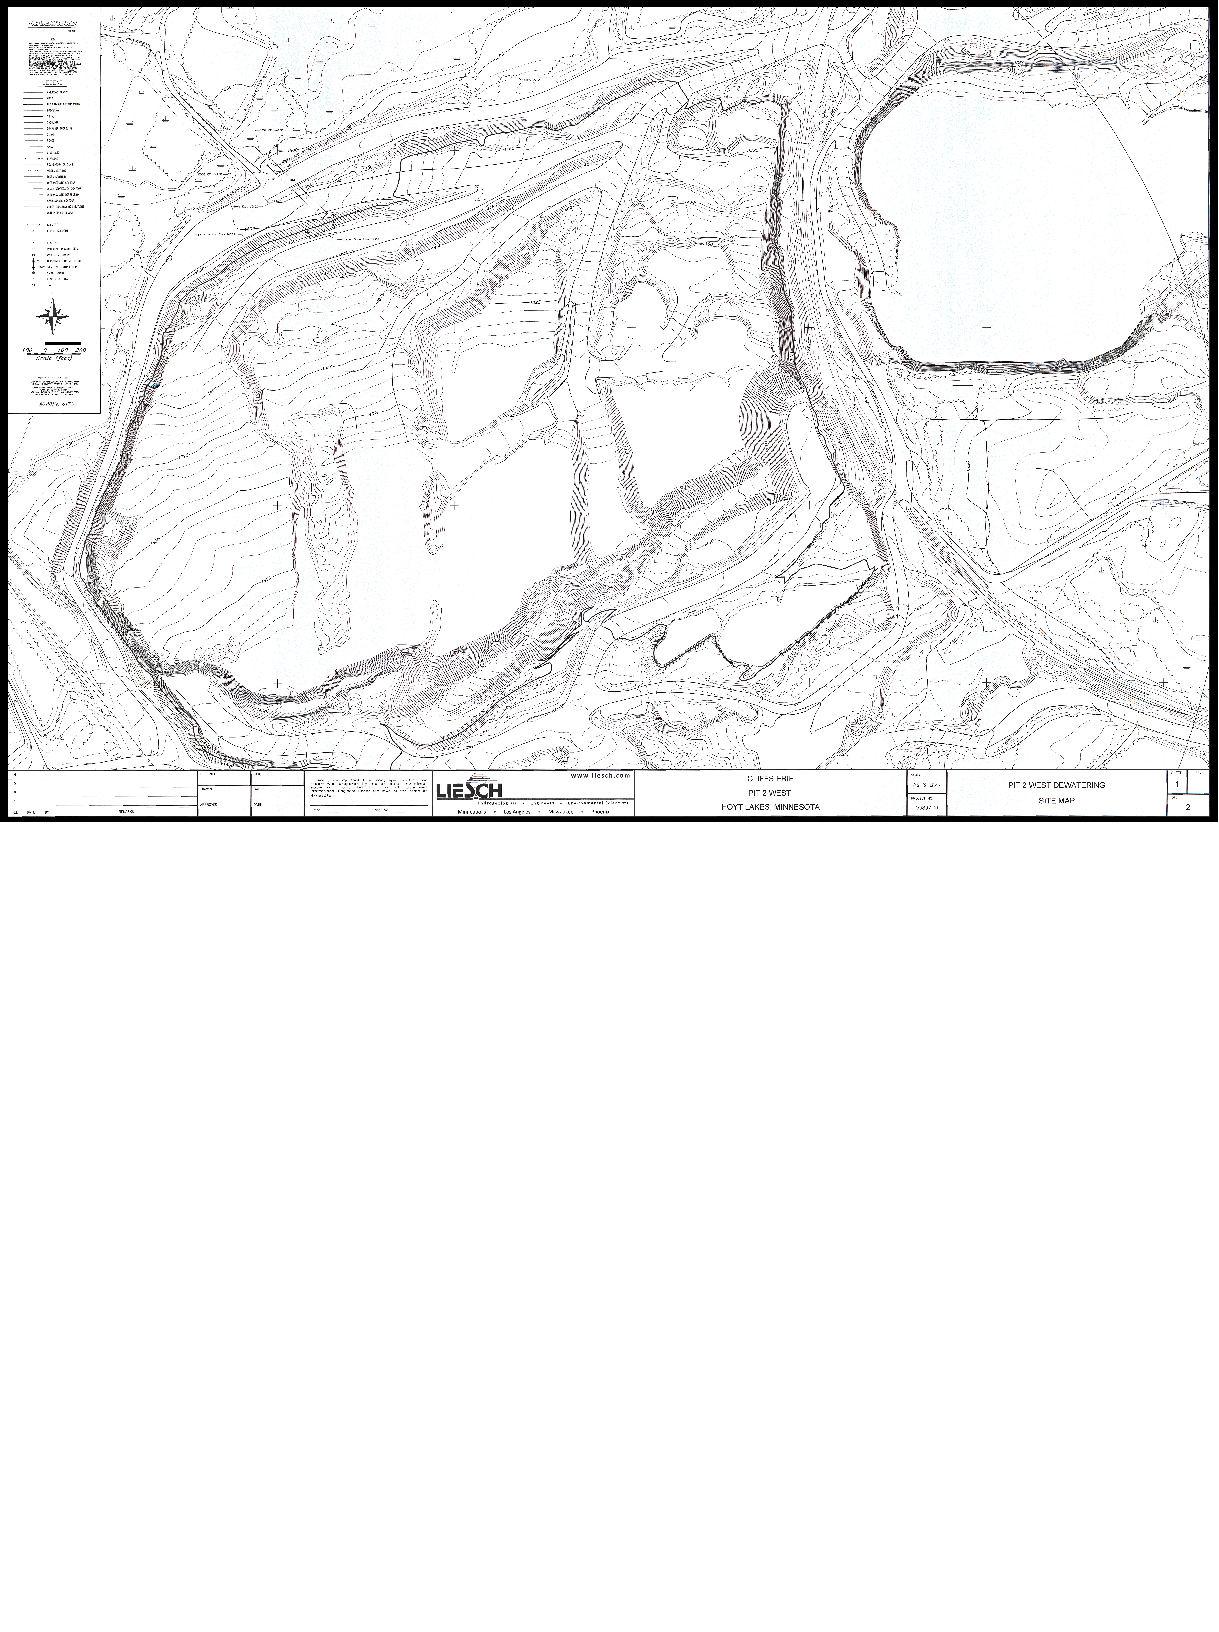
\includegraphics[width=0.6\textwidth]{diagrams/4-chips/contour_map.pdf}
    \caption[Topographic map of the Wentworth 2W mine pit.]
    {Topographic map of the Wentworth 2W mine pit. The contours are given in intervals of 5 feet,
        with the central areas of the pit having a depth of 50m. Image taken from
        Ref.\cite{adamson2013}.}
    \label{fig:contour_map}
\end{figure}

\begin{figure} % CHIPS LOCATION IN NUMI DIAGRAM %
    \includegraphics[width=0.6\textwidth]{diagrams/4-chips/numi_map.png}
    \caption[Map of detector locations in the \numi beam.]
    {Map of the \chips, NoVA and MINOS locations in the \numi beam showing the expected
        neutrino event rates, assuming no oscillations. Lines of constant L/E are shown by the
        contours. Image taken from Ref.\cite{adamson2013}.}
    \label{fig:numi_map}
\end{figure}

\subsection{Structure} %%%%%%%%%%%%%%%%%%%%%%%%%%%%%%%%%%%%%%%%%%%%%%%%%%%%%%%%%%%%%%%%%%%%%%%%%%%
\label{sec:chips_detector_structure} %%%%%%%%%%%%%%%%%%%%%%%%%%%%%%%%%%%%%%%%%%%%%%%%%%%%%%%%%%%%%

\begin{figure} % CHIPS RENDER 1 DIAGRAM %
    \includegraphics[width=0.6\textwidth]{diagrams/4-chips/chips_render_1.png}
    \caption[Graphical rendering of the \chipsfive detector with liner cutaway.]
    {Graphical rendering of the \chipsfive detector with a section of the liner cutaway.
        The bottom endcap and wall planes are visable,
        as well as the top endcap structure and floatation.}
    \label{fig:chips_render_1}
\end{figure}

\begin{figure} % CHIPS RENDER 2 DIAGRAM %
    \includegraphics[width=0.6\textwidth]{diagrams/4-chips/chips_render_2.png}
    \caption[Graphical rendering of the \chipsfive detector structure.]
    {Graphical rendering of the \chipsfive detector structure.}
    \label{fig:chips_render_2}
\end{figure}

\subsection{Instrumentation} %%%%%%%%%%%%%%%%%%%%%%%%%%%%%%%%%%%%%%%%%%%%%%%%%%%%%%%%%%%%%%%%%%%%%
\label{sec:chips_detector_instrumentation} %%%%%%%%%%%%%%%%%%%%%%%%%%%%%%%%%%%%%%%%%%%%%%%%%%%%%%%

km3net 2.0 ref in \cite{adrian2016}
Icecube DOM paper \cite{hanson2006}

DIAGRAM: POM diagram
REF: Km3net optical module paper
REF: Nemo-3 PMT paper
- CHIPS uses high quantum efficiency PMTs from Hamamatsu
REF: Get hamamatsu PMT reference
- We will talk in detail about DAQ in the following chapter
- For calibration "flashers" are built into the detector to allow for known location light
generation to calibrate final PMT positions and time resolutuions.

\begin{figure} % PMT ASSEMBLY DIAGRAM %
    \centering
    \subcaptionbox{pmt disassembled\label{fig:pmt_disassembled}}{%
        \includegraphics[height=5cm]{diagrams/4-chips/pmt_disassembled.jpg}%
    }
    \quad
    \subcaptionbox{pmt assembled\label{fig:pmt_assembled}}{%
        \includegraphics[height=5cm]{diagrams/4-chips/pmt_assembled.jpg}%
    }
    \caption[The caption]
    {The caption}
\end{figure}

\begin{figure} % NIKHEF PLANE DIAGRAM %
    \includegraphics[width=0.8\textwidth]{diagrams/4-chips/single_plane.jpg}
    \caption[Picture of a single `Nikhef' plane.]
    {Picture of a single `Nikhef' high density top endcap plane. Both the inward facing and veto
        PMTs can be seen as well as the planes umbilical with the green tape attached.}
    \label{fig:single_plane}
\end{figure}

\subsection{Water clarity} %%%%%%%%%%%%%%%%%%%%%%%%%%%%%%%%%%%%%%%%%%%%%%%%%%%%%%%%%%%%%%%%%%%%%%%
\label{sec:chips_detector_water} %%%%%%%%%%%%%%%%%%%%%%%%%%%%%%%%%%%%%%%%%%%%%%%%%%%%%%%%%%%%%%%%%

- Though remarkably clear the Wentworth pit water is not clean enough for the detector volume
where we require ~30m attenuation length.
- CHIPS attenuation length paper~\cite{amat2017}

\subsection{Deployment} %%%%%%%%%%%%%%%%%%%%%%%%%%%%%%%%%%%%%%%%%%%%%%%%%%%%%%%%%%%%%%%%%%%%%%%%%%
\label{sec:chips_detector_deployment} %%%%%%%%%%%%%%%%%%%%%%%%%%%%%%%%%%%%%%%%%%%%%%%%%%%%%%%%%%%%

DIAGRAM: Floating dock diagram
DIAGRAM: Deployment diagram
- How it can grow if needed

\subsection{Current status} %%%%%%%%%%%%%%%%%%%%%%%%%%%%%%%%%%%%%%%%%%%%%%%%%%%%%%%%%%%%%%%%%%%%%%
\label{sec:chips_detector_status} %%%%%%%%%%%%%%%%%%%%%%%%%%%%%%%%%%%%%%%%%%%%%%%%%%%%%%%%%%%%%%%%

\section{Monte Carlo event generation and simulation} %%%%%%%%%%%%%%%%%%%%%%%%%%%%%%%%%%%%%%%%%%%%
\label{sec:chips_monte_carlo} %%%%%%%%%%%%%%%%%%%%%%%%%%%%%%%%%%%%%%%%%%%%%%%%%%%%%%%%%%%%%%%%%%%%

\subsection{Beam event generation} %%%%%%%%%%%%%%%%%%%%%%%%%%%%%%%%%%%%%%%%%%%%%%%%%%%%%%%%%%%%%%%
\label{sec:chips_monte_carlo_beam} %%%%%%%%%%%%%%%%%%%%%%%%%%%%%%%%%%%%%%%%%%%%%%%%%%%%%%%%%%%%%%%

\begin{figure} % CHIPS FLUX DIAGRAM %
    \includegraphics[width=0.6\textwidth]{diagrams/4-chips/flux.pdf}
    \caption[\numi neutrino flux at CHIPS.]
    {The \numi beam neutrino flux with cross-sections applied at the CHIPS detector location. Shown
        are the seperate contributions from the different neutrino types and sign. No oscillations
        have been applied.}
    \label{fig:flux}
\end{figure}

Cosmic event rate in \cite{son2013}

- We take full advantage of the MINOS, NOVA extensive simulations of the \numi beam for use in
CHIPS.
- The tau neutrino component is negligible and not predicted by the simulation
INFO: expected number of events per year etc...

\subsection{Cosmic event generation} %%%%%%%%%%%%%%%%%%%%%%%%%%%%%%%%%%%%%%%%%%%%%%%%%%%%%%%%%%%%%
\label{sec:chips_monte_carlo_cosmic} %%%%%%%%%%%%%%%%%%%%%%%%%%%%%%%%%%%%%%%%%%%%%%%%%%%%%%%%%%%%%

DIAGRAM: expected cosmic rate at different height plot
DIAGRAM: Cosmic rate given the water overburden diagram

\begin{figure} % COSMICS AROUND DETECTOR DIAGRAM %
    \includegraphics[width=0.8\textwidth]{diagrams/4-chips/cosmics.png}
    \caption[Cosmic muon rays around the CHIPS detector]
    {Simulated cosmic muon rays around the CHIPS detector. Note how they are generated within a
        box.}
    \label{fig:cosmics}
\end{figure}

\subsection{Detector simulation} %%%%%%%%%%%%%%%%%%%%%%%%%%%%%%%%%%%%%%%%%%%%%%%%%%%%%%%%%%%%%%%%%
\label{sec:chips_monte_carlo_sim} %%%%%%%%%%%%%%%%%%%%%%%%%%%%%%%%%%%%%%%%%%%%%%%%%%%%%%%%%%%%%%%%

\begin{figure} % SIMULATED EVENT DISPLAY DIAGRAM %
    \includegraphics[width=\textwidth]{diagrams/4-chips/sim_event.png}
    \caption[sim event short]
    {$\nu_{\mu}$ CC quasi-elastic event with a single muon final state particle of energy
        1770.24 MeV}
    \label{fig:sim_event}
\end{figure}

\begin{figure} % DIGI DIAGRAM %
    \centering
    \subcaptionbox{\label{fig:digi_method}}{%
        \includegraphics[height=6cm]{diagrams/4-chips/digi_method.pdf}%
    }
    \quad
    \subcaptionbox{\label{fig:digi_likelihood}}{%
        \includegraphics[height=6cm]{diagrams/4-chips/digi_likelihood.pdf}%
    }
    \caption[Simulation PMT digitisaion function.]
    {(a) Digitisation function used within the simulation to convert incident photons to measured
        digitised charge. (b) Likelihood of a measured digitised charge being caused by a number
        of photons incident on a PMT.}
    \label{fig:digitisation}
\end{figure}

  \chapter{Data acquisition for CHIPS} %%%%%%%%%%%%%%%%%%%%%%%%%%%%%%%%%%%%%%%%%%%%%%%%%%%%%%%%%%%%%
\label{chap:daq} %%%%%%%%%%%%%%%%%%%%%%%%%%%%%%%%%%%%%%%%%%%%%%%%%%%%%%%%%%%%%%%%%%%%%%%%%%%%%%%%%

The primary task of any Data Acquisition system is the processing of low-level signals measuring
real-world physics and their transfer to permanent storage for further analysis. Commonly, this
procedure also includes decision making as to whether the signal is deemed interesting enough to
record, known as a \emph{trigger}. Both these tasks can make DAQ systems incredibly complex,
especially when they must operate in an efficient and resilient manner for vast amounts of data in
real-time, while also providing detector control and monitoring.

In the context of the \chips project, the DAQ system records all PMT hits, timestamps them using a
common clock, and transfers them out of the detector to a central processing node. This node then
applies a trigger to select hits that fall within the interesting \numi beam spill time window,
before the selected hits are sliced into events and moved to permanent storage for further
analysis. Alongside these processes, the DAQ also configures the whole detector and provides data
quality and detector component monitoring.

Although relatively simple when compared to the incredibly complex and time-pressured DAQ systems
of the LHC experiments, the DAQ system developed for the \chips project introduces some novel
approaches to solve the unique constraints of the \chips concept. Namely, deployment within a body
of water and a limited resource budget. In this chapter, the DAQ system for \chips as applied to
the \chipsfive prototype detector module is described alongside highlighting any novel approaches.
The description is presented in two broad categories, hardware and software, with a short
description of the timing system beforehand.

\section{White Rabbit timing} %%%%%%%%%%%%%%%%%%%%%%%%%%%%%%%%%%%%%%%%%%%%%%%%%%%%%%%%%%%%%%%%%%%%
\label{sec:daq_timing} %%%%%%%%%%%%%%%%%%%%%%%%%%%%%%%%%%%%%%%%%%%%%%%%%%%%%%%%%%%%%%%%%%%%%%%%%%%

To ensure PMT hit times are synchronised throughout \chips detectors, a common clock must be
shared across all timestamping electronics. For this purpose, \chips uses a \emph{White Rabbit}
(WR) network~\cite{lipinski2011}. Initially developed at CERN, the open-source WR project provides
an ethernet-based time distribution network with sub-nanosecond synchronisation accuracy between
nodes. By using two-way exchanges of WR messages, precise adjustment of individual node clock
phases and offsets is possible across thousands of devices, separated by tens of kilometres. All
of this is achieved in parallel with a standard data transfer network capable of
\unit{1}{\text{Gb}} speeds.

All nodes are synchronised to the clock of a \emph{GrandMaster} node, typically a WR
\emph{switch}, the most common WR hardware component. As input, the switch receives an IRIG-B
(Inter-Range Instrumentation Group timecode B) and a \unit{10}{\text{MHz}} signal from a GPS
disciplined oscillator. These inputs allow for synchronisation of the GrandMaster clock to
International Atomic Time (TAI). As \chips detector modules require synchronisation to accelerator
clocks many hundreds of kilometres to determine the arrival time of beam spills accurately, the
GPS disciplined timing is particularly important.

WR hardware is commercially available from many vendors. Within \chipsfive, two WR devices are
used for time synchronisation and data transfer, both shown in Fig.~\ref{fig:wr_electronics}.
Firstly, a compact version of the standard WR switch~\cite{wrswitch2020}, specially developed for
the \chips project at Nikhef~\cite{wrchromium2020}. Secondly, a WR-LEN (Lite Embedded Node) from
Seven Solutions~\cite{wrlen2020}. All WR components are connected using \unit{1}{\text{Gb}}
bi-directional optical fibre connections, using the \unit{1310}{\text{nm}} and
\unit{1550}{\text{nm}} wavelengths via Small Form-Factor Pluggable Transceivers (SFPs).

\begin{figure} % WHITE-RABBIT COMPONENTS DIAGRAM %
    \centering
    \subcaptionbox{White Rabbit switch}{%
        \includegraphics[height=6cm]{diagrams/5-daq/wr_switch.pdf}%
    }
    \quad
    \subcaptionbox{White Rabbit LEN}{%
        \includegraphics[height=6cm]{diagrams/5-daq/wr_len.pdf}%
    }
    \caption[Pictures of the White Rabbit timing hardware used within \chipsfive.]
    {Pictures of the White Rabbit timing hardware used within \chipsfive. The compact White rabbit
        switch  specially designed for \chips is shown in (a), while the White Rabbit Lite
        Embedded Node (WR-LEN) from Seven Solutions is shown in (b).}
    \label{fig:wr_electronics}
\end{figure}

Fig.~\ref{fig:sync} shows the WR synchronised pulse per second clock rising edges for two
\chipsfive WR switches separated by \unit{500}{\text{m}} of fibre. With the vertical ticks
representing single nanoseconds, sub-nanosecond time synchronisation accuracy between the switches
is observed.

\begin{figure} % WHITE-RABBIT SYNC DIAGRAM %
    \includegraphics[width=0.7\textwidth]{diagrams/5-daq/sync.pdf}
    \caption[Picture of White Rabbit timing synchronisation seen in \chips.]
    {Picture of an oscilloscope display measuring the pulse per second output signal from two WR
        switches shown in pink and yellow at either end of a \unit{500}{\text{m}} long optical
        fibre. The vertical ticks are in nanoseconds showing the sub-nanosecond synchronisation
        possible with the WR timing network.}
    \label{fig:sync}
\end{figure}

\section{Hardware} %%%%%%%%%%%%%%%%%%%%%%%%%%%%%%%%%%%%%%%%%%%%%%%%%%%%%%%%%%%%%%%%%%%%%%%%%%%%%%%
\label{sec:daq_hard} %%%%%%%%%%%%%%%%%%%%%%%%%%%%%%%%%%%%%%%%%%%%%%%%%%%%%%%%%%%%%%%%%%%%%%%%%%%%%

The hardware of the \chipsfive DAQ system is split into two distinct implementations at its lower
levels (closest to the PMTs), corresponding to the Nikhef and Madison \textsc{Pom} types. \chips
R\&D efforts have principally developed the novel Madison implementation with the view to use this
hardware within detector modules exclusively. However, as a safe stepping stone, while development
and testing are still ongoing, \chipsfive mainly contains proven Nikhef hardware developed for the
KM3NeT experiment~\cite{adrian2016}.

The complete DAQ and power distribution system for \chipsfive is diagrammatically shown in
Fig.~\ref{fig:daq}. The following subsections describe each component, starting from the lowest
level and working upwards. The Nikhef and Madison descriptions are separated for clarity as well
as the high-level combined hardware systems, part of which is not physically located within the
detector but onshore in an electronics hut (separate from the water filtration hut).

\begin{figure} % DAQ DIAGRAM %
    \includegraphics[width=\textwidth]{diagrams/5-daq/daq.pdf}
    \caption[Diagram of the complete \chipsfive data acquisition and power distribution system.]
    {Diagram of the complete \chipsfive DAQ and power distribution system.}
    \label{fig:daq}
\end{figure}

Common to both low-level hardware implementations is the use of the Time over Threshold (ToT)
method for PMT signal digitisation. Each analogue PMT pulse is fed to a ToT discriminator coupled
with a Time to Digital Converter (TDC) in order to generate each digitised recorded hit, as shown
in Fig.~\ref{fig:tot}. Compared to the more common Analogue to Digital Converter (ADC) readout,
ToT values are less accurate and do not scale linearly with deposited charge. However, the ToT
methodology is used within \chips as the electronics is simpler and notably cheaper.

\begin{figure} % TOT DIAGRAM DIAGRAM %
    \includegraphics[width=0.6\textwidth]{diagrams/5-daq/tot.pdf}
    \caption[Illustrative diagram showing how Time over Threshold is measured.]
    {Illustrative diagram showing how a ToT value is measured. As soon as the rising edge of a PMT
        charge pulse rises above a given threshold (goes below in the negative charge case) a time
        is recorded $t_{1}$, when the falling edge later falls below the threshold a second time
        $t_{2}$ is recorded. The difference in time between $t_{1}$ and $t_{2}$ is output by the
        electronics as a digitised ToT value.}
    \label{fig:tot}
\end{figure}

\subsection{Nikhef hardware} %%%%%%%%%%%%%%%%%%%%%%%%%%%%%%%%%%%%%%%%%%%%%%%%%%%%%%%%%%%%%%%%%%%%%
\label{sec:daq_hard_Nikhed} %%%%%%%%%%%%%%%%%%%%%%%%%%%%%%%%%%%%%%%%%%%%%%%%%%%%%%%%%%%%%%%%%%%%%%

All Nikhef HZC PMTs are attached directly to a simple readout board containing a high-voltage
generating Cockcroft-Walton circuit. Up to 30 such PMTs are connected to two \emph{Calamares}
boards within the electronics box of each Nikhef \textsc{Pom} via standard category 5 cables with
RJ45 connectors, as shown in Fig.~\ref{fig:nikhef_plane}. Both Calamares boards are directly
attached to a \emph{Central Logic Board} (CLB)~\cite{biagi2015, eijk2015}. The CLB contains ToT
discriminators and TDCs to digitise the recorded signals as well as electronics to synchronise to
the WR network clock for timestamping. Each Nikhef \textsc{Pom} electronics box also contains an
AC to DC power converter (AC/DC) whose output is fed into the CLB for distribution.

\begin{figure} % NIKHEF PLANE DIAGRAM %
    \includegraphics[width=0.8\textwidth]{diagrams/5-daq/nikhef_plane.pdf}
    \caption[Labelled picture of the Nikhef \textsc{Pom} electronics box.]
    {Labelled picture of the Nikhef \textsc{Pom} electronics box. Both ends of the category 5 PMT
        cables can be seen, either at the PMT mounting points or entering the electronics box and
        not yet plugged into Calamares boards.}
    \label{fig:nikhef_plane}
\end{figure}

Every Nikhef \textsc{Pom} is connected via a single optical fibre and a single power connection to
a \emph{Nikhef-container}, the contents of which are labelled in the bottom half of
Fig.~\ref{fig:full_setup}. Two WR switches are used within each container to provide sufficient
\textsc{Pom} networking ports. Both switches are powered by independent AC to DC converters and
connected via a single optical fibre each to the higher level DAQ systems. An additional
connection between each switch ensures that if one higher-level connection fails the other can
still be used.

Each Nikhef-container also contains a relay board to control the power supply to individual
\textsc{Pom}s. The relay board control electronics are powered via an AC to DC converter and
connected to one of the switches via a media converter for networking. The media converter is
required to convert the optical fibre WR switch connection to a standard RJ45 copper cable
connection. A total of five Nikhef-containers are present within \chipsfive.

\begin{figure} % FULL SETUP DIAGRAM %
    \includegraphics[width=\textwidth]{diagrams/5-daq/full_setup.pdf}
    \caption[Picture of the non \textsc{Pom} components of the \chipsfive DAQ system]
    {Picture of the non \textsc{Pom} components of the \chipsfive DAQ system arranged on a table
        at the PolyMet mining administration building.}
    \label{fig:full_setup}
\end{figure}

\subsection{Madison hardware} %%%%%%%%%%%%%%%%%%%%%%%%%%%%%%%%%%%%%%%%%%%%%%%%%%%%%%%%%%%%%%%%%%%%
\label{sec:daq_hard_madison} %%%%%%%%%%%%%%%%%%%%%%%%%%%%%%%%%%%%%%%%%%%%%%%%%%%%%%%%%%%%%%%%%%%%%

Every Madison Hamamatsu PMT is directly attached to a high-voltage generating Cockcroft-Walton
board followed by a signal processing \emph{$\micro$DAQ}, as shown in
Fig.~\ref{fig:madison_pmt_assembly}. The $\micro$DAQ is a small microcontroller developed for both
IceCube and \chips at WIPAC in Madison. Capable of timestamping and digitising signals directly at
the PMT level, the $\micro$DAQ also sets the PMT operating voltage by controlling the driving
frequency of the Cockcroft-Walton board~\cite{eijk2018}.

Up to 16 $\micro$DAQs receive power, networking, and WR synchronised IRIG-B and
\unit{10}{\text{MHz}} timing signals from a \emph{badger-board}, as shown in
Fig.~\ref{fig:madison_plane}. Standard category 5 cables with RJ45 connectors are used for these
connections. The badger-board is located within the electronics box of each Madison \textsc{Pom}
and acts as a simple fanout and power control board. For logic, each badger-board has an attached
mezzanine Beaglebone~\cite{beagle2020}. This single-board Linux machine (very similar to a
Raspberry Pi) controls the power supply to, and receives hits from, the attached $\micro$DAQs.

\begin{figure} % MADISON PLANE DIAGRAM %
    \includegraphics[width=0.8\textwidth]{diagrams/5-daq/madison_plane.pdf}
    \caption[Labelled picture of the components of the Madison \textsc{Pom} electronics box.]
    {Labelled picture of the components of the Madison \textsc{Pom} electronics box.}
    \label{fig:madison_plane}
\end{figure}

Similarly, up to 16 Madison \textsc{Pom} badger-boards receive power, networking and WR
synchronised IRIG-B and \unit{10}{\text{MHz}} timing signals from a \emph{danout-board} located
within a single \emph{Madison-container}. Again, standard category 5 cables with RJ45 connectors
are used for these connections. The full contents of the Madison-container are shown in
Fig.~\ref{fig:madison_box}. Similar to the badger-board, the danout-board acts as a simple fanout
and power control board with an attached mezzanine Beaglebone. However, in this case, the attached
Beaglebone acts only to control the power provided by the danout-board.

PMT hits and other packets are instead routed through the danout-board into a networking stack.
Consisting of a WR-LEN, a router (required due to the limited WR-LEN routing table size), and a
switch (non WR), the stack provides networking to the higher-level DAQ via a single optical fibre.
The WR clock synchronised IRIG-B and \unit{10}{\text{MHz}} timing signals are output by the WR-LEN
to the danout-board for forwarding to the lower-level components. Additionally, two AC to DC
converters provide power for both the devices within the container and all lower-level components
via the danout-board.

\begin{figure} % MADISON BOX DIAGRAM %
    \includegraphics[width=\textwidth]{diagrams/5-daq/madison_box.pdf}
    \caption[Labelled picture of the Madison-container components.]
    {Labelled picture of the Madison-container components. The blue and grey cables exiting the
        left hand side of the image go to individual Madison \textsc{Pom}s connecting to the I/O
        port shown in fig.~\ref{fig:madison_plane}. An optical fibre connection into the left SFP
        port of the WR-LEN is used in reality rather than the copper connection shown here.}
    \label{fig:madison_box}
\end{figure}

Compared to the Nikhef hardware the Madison.
\begin{itemize}
    \item By leveraging commercially available Beaglebones ($\sim£50$ each) for onboard logic and
    using vastly \textbf{cheaper} WR-LENs compared to WR switches, the Madison DAQ hardware
    implementation is drastically cheaper compared to the Nikhef (KM3NeT) approach for a minimal
    reduction in performance.
    \item By having a fully fledged Linux machine on each POM and easily reprogrammable
    $\micro$DAQ microcontrollers the DAQ software can be easily \textbf{configurable} and upgraded
    once deployed. Having so much cheap general purpose processing power close to the PMTs allows
    for most of the computation to happen at that level, additional logic can be added. Don't even
    know what we could implement yet using it. Advanced processing at lower level. 
\end{itemize}

\subsection{Combined systems} %%%%%%%%%%%%%%%%%%%%%%%%%%%%%%%%%%%%%%%%%%%%%%%%%%%%%%%%%%%%%%%%%%%%
\label{sec:daq_hard_combined} %%%%%%%%%%%%%%%%%%%%%%%%%%%%%%%%%%%%%%%%%%%%%%%%%%%%%%%%%%%%%%%%%%%%

Each Nikhef-container and Madison-container is connected to a single \emph{junction-box}, labelled
in Fig.~\ref{fig:full_setup}. This central container acts as the interface between the detector
electronics and the umbilical carrying data and power between the shore and the detector. All
connections to the junction-box (as well as those between \textsc{Pom}s and Nikhef and Madison
containers) are made within watertight, flexible PVC tubing called \emph{manifolds}. These tubes
span all corners of the \chipsfive detector, as shown in Fig.~\ref{fig:manifold}.

\begin{figure} % MANIFOLD DIAGRAM %
    \includegraphics[width=\textwidth]{diagrams/5-daq/manifold.pdf}
    \caption[manifold short]
    {Picture of a Nikhef \textsc{Pom} to Nikhef-container manifold (in white) attached to the
        top-cap of the \chipsfive detector. In the left of the image, two unattached Nikhef
        \textsc{Pom} pigtail connections are seen, both covered in green tape and a plastic bag.}
    \label{fig:manifold}
\end{figure}

For networking the junction-box contains a Coarse Wavelength Division Multiplexing (CWDM)
multiplexer/demultiplexer (MUX/DEMUX). This device supports 32 wavelengths for a total of 16
bi-directional \unit{1}{\text{Gb}} connections over the single \unit{500}{\text{m}} long umbilical
optical fibre. Each WR-LEN or WR switch within the detector uses one of these channels exclusively
with the corresponding wavelength SFP.

The two umbilical power connections are distributed via two thick copper plates to all the relay
channels within the junction-box. Two relay boards are used to provide a sufficient number of
output channels, with their control electronics powered by separate AC to DC converters and each
connected to one of the multiplexer/demultiplexer networking channels via a media converter
(optical fibre to RJ45). Each relay channel also has a built-in \emph{trip gate} to immediately
power-off the channel if a current surge is detected. This protection is particularly crucial for
\chipsfive as water leaks are a possibility.

The contents of the DAQ electronics \emph{Shore Hut} are shown in Fig.~\ref{fig:hut_daq}. The
single umbilical optical fibre connection passes through a multiplexer/demultiplexer before each
of the wavelength-specific channels are passed into one of two WR switches to provide sufficient
ports. Multiple Virtual Local Area Networks (VLANs) are configured on each switch such that for
each wavelength channel only a single paired port on the other physical side of the switch carries
that channels data to and from the standard networking switch. Of the two WR switches, one is
configured to be the GrandMaster with connections to a GPS disciplined oscillator (with antenna).
A single connection is also made between the WR switches for clock synchronisation.

\begin{figure} % WHITE-RABBIT GM SETUP DIAGRAM %
    \includegraphics[width=\textwidth]{diagrams/5-daq/hut_daq.pdf}
    \caption[Picture of the onshore components of the \chipsfive DAQ system]
    {Picture of the onshore components of the \chipsfive DAQ system arranged on a table at the
        PolyMet mining administration building.}
    \label{fig:hut_daq}
\end{figure}

The standard network switch provides unit{10}{\text{Gb}} connections to each of the Shore DAQ
computing machines whose specific roles are detailed in Section.~\ref{sec:daq_soft}. Each machine
is also connected to a second switch providing connections to the external internet and DAQ
components located at Fermilab.

An uninterruptible power supply provides power to all devices within the Shore Hut, providing
power for up to \unit{15}{\text{minutes}} after a power cut (sadly quite common). The two detector
umbilical power connections do not use the uninterruptible supply and instead draw power directly
from the master supply, as does the water filtration pump.

\section{Data flow and software} %%%%%%%%%%%%%%%%%%%%%%%%%%%%%%%%%%%%%%%%%%%%%%%%%%%%%%%%%%%%%%%%%
\label{sec:daq_soft} %%%%%%%%%%%%%%%%%%%%%%%%%%%%%%%%%%%%%%%%%%%%%%%%%%%%%%%%%%%%%%%%%%%%%%%%%%%%%

TODO: Write the software section of the DAQ chapter

~\cite{chipsdaq2020}

- What makes this implementation special
- Limited resource, but brilliant capabilities
- Use existing software when possible

- Need to talk about what is novel, new and exciting!
- Not so much about the hardcore electronics details, more high level
- FINITE STATE MACHINE!!!

SOFTWARE
- The beam spill
- Hit acquisition and handling
- Detector and data quality monitoring

\begin{figure} % SOFTWARE DIAGRAM %
    \includegraphics[width=\textwidth]{diagrams/5-daq/daq_software.pdf}
    \caption[daq software short]
    {daq software long}
    \label{fig:daq_software}
\end{figure}

- INCLUDE DATA RATES IN SOFTWARE DIAGRAM
- INCLUDE WHICH MACHINES THINGS RUN ON IN SOFTWARE DIAGRAM

- Where the DHCP server is
- Separated into slow-control, data collection, and

- Need to get across what makes this DAQ implementation special and novel, what are the
interesting unique bits of it? Limited resources but great performance! Use of existing hardware
and software! Modern approaches to doing things, good part of small collaboration!
- Needs to able to cope with 4 degrees at bottom!
- Talk about expected data through put, what we can cope with
- Jumbo frames etc

- An `all-data-to-shore' approach as done in KM3NeT
- Data is sent in UDP packets (not TCP so some will go missing)
- $\micro$DAQ software repository with fh-library (field-hub) novel communication library
in~\cite{microdaq2020}. Most of Madison code is written in c!
- Mainly written in C++, full asynchronous using the BOOST Asio library in~\cite{boost2020} which
is a library for network and low-level I/O programming using an asynchronous model.
- Taking inspiration from the KM3NeT DAQ Java software
- The detector is configured using a single human readable configuration file that defines all the
\textsc{Pom} types, MAC addresses, IP addresses, types, relay channels, which channels should be active and
their associate high voltage setting, threshold and electronic ID.
- Typical ethernet frame has a maximum transmission unit (MTU) size of 1500 bytes, we use Jumbo
frames that allow for an MTU of 9000 bytes, this means we have a lot less small frames with only a
limited number of recorded hits, which proved to be taxing to the switches and lead to an increase
in the number of dropped frames.
- 1Gb links between WR switches, 10Gb link between FS switch and main DAQ machine. Provides
sufficient bandwidth, DO A SMALL CALCULATION!

\subsection{Detector control} %%%%%%%%%%%%%%%%%%%%%%%%%%%%%%%%%%%%%%%%%%%%%%%%%%%%%%%%%%%%%%%%%%%%
\label{sec:daq_soft_control} %%%%%%%%%%%%%%%%%%%%%%%%%%%%%%%%%%%%%%%%%%%%%%%%%%%%%%%%%%%%%%%%%%%%%

\subsection{Hit acquisition} %%%%%%%%%%%%%%%%%%%%%%%%%%%%%%%%%%%%%%%%%%%%%%%%%%%%%%%%%%%%%%%%%%%%%
\label{sec:daq_soft_hits} %%%%%%%%%%%%%%%%%%%%%%%%%%%%%%%%%%%%%%%%%%%%%%%%%%%%%%%%%%%%%%%%%%%%%%%%

\subsection{Monitoring} %%%%%%%%%%%%%%%%%%%%%%%%%%%%%%%%%%%%%%%%%%%%%%%%%%%%%%%%%%%%%%%%%%%%%%%%%%
\label{sec:daq_soft_monitor} %%%%%%%%%%%%%%%%%%%%%%%%%%%%%%%%%%%%%%%%%%%%%%%%%%%%%%%%%%%%%%%%%%%%%

- Elasticsearch ref in~\cite{elastic2020}
- An open source RESTful, JSON-based, search engine and noSQL database.
- Data is stored in \emph{indices} in individual \emph{documents}
- Get to leverage an enormous amount of online support and the community
- daqlog: Uses for DAQ application logging with a severity
- daqstate: Used to report the current state of various DAQ applications
- monpom: Used for reporting general \textsc{Pom} monitoring information, such as temp, humidity, status
- monchannel: Used for reporting individual channel monitoring, such as rate, veto
- A series of altering rules are also set up constantly monitoring the status of the monitoring
data contained within the elasticsearch database to alert via slack or email individuals if something goes wrong.
- We index asynchronously to not block data taking, all data is backed up easily.
- Use the Kibana user interface which is accessible through a browser, means that no special
equipment, or GUIs are used, anyone on any machine has access to the full monitoring stack from
their browser. A series of dashboards ar set up to monitor everything within the detector.
- A series of indices are set up to store data which is sent via standard REST messages to the
database, the special indexing allows for quick `searching' over any time period etc... for
monitoring.
- Also means that anyone can quickly/easily look at any part of the data and make plots etc...
without needing to write an additional part of a monitoring program.

\begin{figure} % MONITORING DIAGRAM %
    \includegraphics[width=\textwidth]{diagrams/5-daq/monitoring.pdf}
    \caption[monitoring short]
    {monitoring long}
    \label{fig:monitoring}
\end{figure}
  \chapter{Convolutional neural networks for CHIPS} %%%%%%%%%%%%%%%%%%%%%%%%%%%%%%%%%%%%%%%%%%%%%%%%
\label{chap:cvn} %%%%%%%%%%%%%%%%%%%%%%%%%%%%%%%%%%%%%%%%%%%%%%%%%%%%%%%%%%%%%%%%%%%%%%%%%%%%%%%%%

For the majority of HEP experiments, event analysis entails the separation of signal from
background, identification of particles, discovery of kinematic properties and estimation of
energies. The same is true for \chips, with the primary aims being the selection of CC $\nu_{e}$
signal events from a sizeable background and estimation of the associated neutrino energy.

For this purpose, the \chips project has so far relied on a human implemented reconstruction
algorithm and a classification neural network driven by hand-engineered features. Both of which
are prone to human error and restricted in scope to what has been implemented in software.

The work outlined in this chapter presents a replacement event analysis methodology for \chips.
Three \emph{Convolutional Neural Networks} (CNNs)~\cite{fukushima1982}, a type of \emph{deep
    learning}~\cite{goodfellow2016} neural network have been implemented, primarily to achieve the
goals outlined above. One for cosmic rejection, one for beam classification, and one for neutrino
energy estimation.

After covering previous deep learning implementations for neutrino experiments, a brief
description of the current techniques to be replaced is made. The theoretical background to CNNs
is then outlined before the baseline implementation for \chips is described. Finally, the three
separate networks are detailed, and their combined performance presented.

\section{Previous applications of deep learning for neutrino experiments} %%%%%%%%%%%%%%%%%%%%%%%%
\label{sec:cvn_previous} %%%%%%%%%%%%%%%%%%%%%%%%%%%%%%%%%%%%%%%%%%%%%%%%%%%%%%%%%%%%%%%%%%%%%%%%%

Over the last few years, neutrino experiments have started to adopt deep learning techniques for a
range of tasks. This trend has followed the general explosion of interest in the field amongst the
global research community, especially within computer vision, as can be seen in
Fig.~\ref{fig:papers}.

\begin{figure} % NUMBER OF PAPERS DIAGRAM DIAGRAM %
    \includegraphics[width=0.7\textwidth]{diagrams/6-cvn/papers.png}
    \caption[papers short]
    {The number of artificial intelligence papers submitted to arXiv, broken down by sub-category.
        Note the particularly large increase in Computer Vision (CV) and pattern recognition
        papers. Figure taken from Ref.\cite{perrault2019}.}
    \label{fig:papers}
\end{figure}

In 2016 the \nova experiment applied a CNN to the task of classifying the interaction type of
events within their sampling calorimeter detector~\cite{aurisano2016}. Two views of raw detector
events were used as input to train a network based on the popular GoogLeNet
architecture~\cite{szegedy2015}, discussed in section \ref{sec:cvn_theory_conv}. An improved
iteration has since been applied to both the classification of individual energy deposit
clusters~\cite{psihas2019} and $\nu_{e}$ and $e^{-}$ energy reconstruction~\cite{baldi2019}.

CNNs have also been applied to liquid argon time-projection chambers. The MicroBooNE
experiment~\cite{acciarri2017_ref} has shown that in addition to classification tasks, the
localisation of single particles within events is possible~\cite{acciarri2017}. Furthermore, the
DUNE collaboration has designed a network to output both the interaction class and counts of
different particle types in an event~\cite{collaboration2020, abi2020}. This approach is called
\emph{multi-task} learning and is discussed in detail within
Section.~\ref{sec:cvn_baseline_outputs}.

Applications to water Cherenkov detectors have also been made, by both the Daya Bay reactor
experiment~\cite{racah2016} and the KM3NeT/ORCA collaboration~\cite{aiello2020}. Additionally, a
type of network known as a \emph{variational autoencoder} has been shown to approximate the
distribution of simulated water Cherenkov data~\cite{abhishek2019}. If further studies prove
successful, this could allow for training on real data to reduce experimental uncertainties and
increase the speed of simulated data generation by many orders of magnitude.

\section{Standard event reconstruction and classification} %%%%%%%%%%%%%%%%%%%%%%%%%%%%%%%%%%%%%%%
\label{sec:cvn_old} %%%%%%%%%%%%%%%%%%%%%%%%%%%%%%%%%%%%%%%%%%%%%%%%%%%%%%%%%%%%%%%%%%%%%%%%%%%%%%

It is essential to outline the standard event reconstruction and classification methods that have
been used by the \chips project until now, for two main reasons. Firstly, to add context for
comparison with the new CNN approach, as is done throughout Section.~\ref{sec:cvn_results}.
Secondly, to highlight the main weaknesses of these methods, motivating the new technique and
making its advantages clear.

A \emph{maximum likelihood} method based on that implemented by MiniBooNE~\cite{patterson2009} is
used for event reconstruction. Additionally, a simple neural network built using the TMVA
package~\cite{hocker2007} and using outputs from the reconstruction is used for event
classification. Both methods are very typical of the mainstream approach used by the majority of
water Cherenkov neutrino experiments. A prime example is the fiTQun algorithm developed for the
Super-Kamiokande detector, which is now used for both atmospheric~\cite{jiang2019} and
T2K~\cite{missert2017} analyses.

\subsection{Likelihood based reconstruction} %%%%%%%%%%%%%%%%%%%%%%%%%%%%%%%%%%%%%%%%%%%%%%%%%%%%%
\label{sec:cvn_old_reco} %%%%%%%%%%%%%%%%%%%%%%%%%%%%%%%%%%%%%%%%%%%%%%%%%%%%%%%%%%%%%%%%%%%%%%%%%

The event reconstruction methodology is simple in theory: for a given set of hypothesised tracks,
the number of photoelectrons and the time at which the first of these is recorded for each PMT in
the detector is predicted. By comparing this prediction with the measured hit charges and times
the likelihood that the given track hypothesis produced the measured signals can be calculated.
The parameters that describe the hypothesised tracks are then varied until the negative logarithm
of the likelihood is minimised. Identifying the best-fit parameters for the hypothesis. A brief
description of the procedure is given below, however, for a full description see
Ref.~\cite{blake2016} and in great detail Ref.~\cite{perch2017}.

\subsubsection*{Seeding} %%%%%%%%%%%%%%%%%%%%%%%%%%%%%%%%%%%%%%%%%%%%%%%%%%%%%%%%%%%%%%%%%%%%%%%%%

The first stage of event reconstruction is the effective \emph{seeding} of tracks that are then
used in the full likelihood fit. The seeding methods aim to provide a good starting point for the
minimisation, both to increase the efficiency of finding the optimal track parameters and also to
avoid a false local minimum from being returned.

Firstly, the PMT hits are sliced in both space and time. Gaps in the time ordering of hits are
used to separate the event into time slices. Each of these then undergoes basic filtering and
clustering to remove outlying hits and ensure only the dominant collections of hits are
considered. Each cleaned slice is then run through simple vertex finding algorithms to estimate
the interaction position and time, as well and the initial track direction.

A circular \emph{Hough transform} algorithm, traditionally used for water Cherenkov ring finding
is then applied. The voting-based transformation produces an output space within which rings of
PMT hits exist as single peaks. The track direction values are then further refined using this
space, and a search for smaller peaks is carried out to indicate if multiple particles are likely
to be involved. This process results in a list of seeds with a corresponding score related
directly to the height of the associated peak in Hough transform space.

\subsubsection*{Likelihood fit} %%%%%%%%%%%%%%%%%%%%%%%%%%%%%%%%%%%%%%%%%%%%%%%%%%%%%%%%%%%%%%%%%%%

Each track in a fit hypothesis is made up of a vector of parameters $\vec{x}$, containing the
following:
\begin{itemize}
    \item The track vertex position ($x_{0}$, $y_{0}$, $z_{0}$) and interaction time $t_{0}$.
    \item The initial track direction ($d_{\theta}$, $d_{\phi}$).
    \item The initial kinetic energy of the particle.
    \item The particle type (muon, electron or photon).
\end{itemize}
Additionally, for a photon hypothesis (identical to an electron hypothesis in reality) the
distance between the interaction vertex and the beginning of the electromagnetic shower is
included as a parameter.

The tracks in the hypothesis are then initialised using those found in the seeding procedure in
descending order of Hough peak height score. As the seeding algorithms do not estimate the
particle energy, a default value equal to the average particle energy observed in the Monte Carlo
simulation is assigned. Additionally, constraints can be placed on multi-track fits before the
minimisation process begins to reduce the number of free parameters.

For example, in the NC $\pi^{0}$ case, a multi-track two-photon hypothesis is used. Firstly, the
initial parameters for the two photons are assigned from the two highest-scoring seeds. Secondly,
the vertex position for both tracks is constrained to remain the same, and the directions and
energies are set to be constrained by the invariant mass of the $\pi^{0}$.

In it's simplest form the likelihood is a simple product of two terms:
\begin{equation} % LIKELIHOOD EQUATION %
    \mathcal{L}(\vec{x})=\mathcal{L}_{unhit}(\vec{x})\mathcal{L}_{hit}(\vec{x})=
    \prod_{unhit}P_{unhit}(\vec{x})\prod_{hit}P_{charge}(\vec{x})P_{time}(\vec{x}),
    \label{eq:likelihood}
\end{equation}
where the first ($unhit$) gives the likelihood that the hypothesis $\vec{x}$ will not predict a
hit on the PMTs that do not have a measured hit, and the second ($hit$) gives the likelihood that
$\vec{x}$ produces the observed photoelectrons and hit times on the hit PMTs. By considering the
negative logarithm of the likelihood instead, the computation can be simplified into a sum of
logarithms over the PMTs, such that
\begin{equation} % LIKELIHOOD SUM PMTS EQUATION %
    -\log\mathcal{L}(\vec{x})=
    -\sum_{unhit}\log(P_{unhit}(\vec{x}))
    -\sum_{hit}\log(P_{charge}(\vec{x}))
    -\sum_{hit}\log(P_{time}(\vec{x})).
    \label{eq:likelihood_sum}
\end{equation}
This also has the effect of separating the charge (number of photoelectrons) and time prediction
components which can then be dealt with separately computationally. In the actual likelihood
calculation the $P_{unhit}(\vec{x})$ and $P_{charge}(\vec{x})$ components are combined, where the
probability of an unhit PMT is treated as a PMT with observed charge equal to zero.

The Minuit2 algorithm contained within ROOT software package~\cite{brun1997} is used for the
minimisation process. At each iteration, the charge and hit time predictions are made, and the
negative logarithm of the likelihood is calculated. The track parameters are then varied to
minimise the likelihood before the next iteration. Through a series of stages, fixing and freeing
specific parameters, the minimisation process converges to the best-fit parameters for the given
hypothesis. This process typically takes two minutes on a standard batch farm computing node.

\subsubsection*{Downsides} %%%%%%%%%%%%%%%%%%%%%%%%%%%%%%%%%%%%%%%%%%%%%%%%%%%%%%%%%%%%%%%%%%%%%%%

The charge and hit time predictions and their associated likelihood contributions rely on many
low-level inputs to the reconstruction. These generally describe how Cherenkov light is emitted
from specific particles and then propagates through the detector to be detected by the PMTs.
Examples of these inputs include the following:
\begin{itemize}
    \item The number of Cherenkov photons emitted by a particle of specific type and energy.
    \item The fraction of Cherenkov light emitted at each step along a specific particles track
          length.
    \item The angular distribution of Cherenkov photon emission for each type of particle.
    \item The survival probability of photons within the detector medium as a function of
          distance.
    \item A detailed description of the PMT positions and directions within the detector.
    \item The angular efficiency of each PMT relative to the incident photon angle.
    \item The probability of a measured charge given the predicted number of photoelectrons
          (derived from a reversal of the simulation digitisation methodology).
\end{itemize}
The first three are combined into \emph{emission profiles} generated from a large Monte Carlo
simulation sample, while the last listed input is comparable to that shown in
Fig.~\ref{fig:digitisation}.

The list above demonstrates a fundamental problem with the likelihood-based approach. It is
heavily reliant on the accuracy of low-level inputs and their associated use in human implemented
software. If a physical process is not dealt with appropriately or overlooked (the hadronic
component of events), then the prediction accuracy of charges and hit times for the PMTs is
affected, impacting the performance of finding accurate best-fit parameters.

The other fundamental flaw of the likelihood-based approach is the requirement of a predefined
track hypothesis. Real events expected within \chips are rarely simple single particle or even
two-particle events. In reality, the majority of events contain multiple final state particles of
various types and in various topologies. The predefinition of a track hypothesis makes the
implementation of a generalised approach to event reconstruction where all possible event types
are considered, impossible.

\subsection{Event classification}%%%%%%%%%%%%%%%%%%%%%%%%%%%%%%%%%%%%%%%%%%%%%%%%%%%%%%%%%%%%%%%%%
\label{sec:cvn_old_pid} %%%%%%%%%%%%%%%%%%%%%%%%%%%%%%%%%%%%%%%%%%%%%%%%%%%%%%%%%%%%%%%%%%%%%%%%%%

As the reconstruction is based on the calculation of a likelihood (analogous to a
\emph{goodness-of-fit}), the likelihood ratio between different hypotheses can be used for event
classification tasks. It is also found that additional hand-engineered features derived from the
reconstruction outputs have power in classifying the event type.

Two simple neural networks are used, the first for CC $\nu_{e}$ - CC $\nu_{\mu}$ separation and
the second for CC $\nu_{e}$ - NC separation. Both contain a single hidden layer, with the number
of nodes equal to the number of input parameters plus five. Variables from both a single $e$
track, and single $\mu$ track hypothesis fit to each event are used for both networks, with a full
list of inputs as follows:
\begin{itemize}
    \item The $\Delta\log\mathcal{L}$ between $e$ and $\mu$ hypothesis for both time and charge
          components.
    \item The total number of hit PMTs ($N_{hits}$) and total collected charge.
    \item $\frac{\Delta\log\mathcal{L}_{charge}}{N_{hits}}$.
    \item The fraction of hits inside, within, and outside the ring for both $e$ and $\mu$
          hypotheses.
    \item The fraction of predicted charge outside the ring for both $e$ and $\mu$ hypotheses.
    \item The ratio of the total predicted charged to the total measured charge for both $e$
          and $\mu$ hypothesis.
    \item The ratio of the reconstructed energy to the total measured charge.
    \item The reconstructed track direction under the $e$ hypothesis.
    \item The fraction of hits in the downstream half of the detector.
    \item The number of seeds generated by the Hough transform seeding algorithm.
    \item The peak height score of the first and last seeds found by the Hough transform seeding
          algorithm.
\end{itemize}

A sample of CC $\nu_{e}$ and CC $\nu_{\mu}$ beam events characteristic of those expected to be
seen by \chips is used to train the first classifier, and a corresponding sample of CC $\nu_{e}$
and NC events for the second. Both output values can then be used to select CC $\nu_{e}$ events
from the backgrounds. Note that only this primary selection has been implemented, no CC
$\nu_{\mu}$ selection has been developed.

The main limitation of this approach is that the input features are restricted to those that have
been imagined (requiring extensive domain knowledge) and then implemented in software. The current
list is undoubtedly non-exhaustive of all the possible variables and combinations of variables
that can, in theory, be used for discrimination between events. Additionally, any mistakes in the
likelihood-based reconstruction and, therefore, input variables to the neural networks, can lead
to incorrect categorisation of events.

\section{The theory of neural networks} %%%%%%%%%%%%%%%%%%%%%%%%%%%%%%%%%%%%%%%%%%%%%%%%%%%%%%%%%%
\label{sec:cvn_theory} %%%%%%%%%%%%%%%%%%%%%%%%%%%%%%%%%%%%%%%%%%%%%%%%%%%%%%%%%%%%%%%%%%%%%%%%%%%

There are many machine learning techniques: linear regression, logistic regression, k-nearest
neighbours, decision trees, random forests, support vector machines, all of which learn to make
predictions about data. However, none have been as successful, especially in recent years, as the
deep neural network. As both the size of datasets and the amount of available computational power
has increased, deep neural networks have proven the most powerful technique for many tasks as they
are well suited to this paradigm.

Here we discuss the application of neural networks for \emph{supervised learning}, one of two
broad machine learning categories that is concerned with using labelled example data to train
algorithms. The other category of \emph{unsupervised learning}, where the properties of the
dataset are inferred without example data is not discussed, however, will be used for trained
network \emph{explainability} in Section.~\ref{sec:cvn_explain}.

\subsection{Neural network basics} %%%%%%%%%%%%%%%%%%%%%%%%%%%%%%%%%%%%%%%%%%%%%%%%%%%%%%%%%%%%%%%
\label{sec:cvn_theory_basics} %%%%%%%%%%%%%%%%%%%%%%%%%%%%%%%%%%%%%%%%%%%%%%%%%%%%%%%%%%%%%%%%%%%%

A neural network is a type of algorithm inspired by the repeating cell structure of neurons within
our brains. The basic building block of a neural network is a \emph{neuron} which takes a vector
of $k$ inputs $\vec{x} = (x_{1}, x_{2},\dots,x_{k})$ and outputs a scalar $a(\vec{x})$. The
neurons are arranged into layers, with the input of one layer being the output from the previous
layer. The first layer is commonly referred to as the \emph{input layer}, the middle layers as
\emph{hidden layers}, and the final layer as the \emph{output layer}, as illustrated in
Fig.~\ref{fig:network}. In general, this simple neural network structure is referred to as
\emph{fully-connected} as all the neurons in each layer have connections to all the neurons in the
previous and following layers.

\begin{figure} % BASIC NETWORK DIAGRAM %
    \includegraphics[width=0.7\textwidth]{diagrams/6-cvn/network.pdf}
    \caption[Illustration of a simple neural network]
    {Illustration of a simple neural network. There is a single input layer (yellow), two hidden
        layers (blue), and an output layer (green). Each node corresponds to a \emph{neuron}
        except for the input layer.}
    \label{fig:network}
\end{figure}

Input variables (traditionally hand-engineered features extracted from the raw data) are passed
into the network via the input layer. Any number of hidden layers containing any number of neurons
can then follow. The neurons contained within these layers are trained so that collectively their
$a(\vec{x})$ functions solve the task at hand. For a \emph{regression} task, the output layer
outputs a continuous decimal value. Otherwise, for a \emph{classification} task, a probability
value between zero and one is output for each class. The forward passing of information from one
layer to the next is why neural networks can also be referred to as \emph{feed-forward graphs}.

For a neuron $i$, $a_{i}(\vec{x})$ can be decomposed into a linear operation, specific to the
neuron, followed by a non-linear operation, which is the same across all neurons. The linear
operation consists of the dot product of the input vector $\vec{x}$ with a vector of weights
$\vec{w}^{(i)} = (w_{1}^{(i)}, w_{2}^{(i)},\dots,w_{k}^{(i)})$, plus a bias term $b^{(i)}$:
\begin{equation} % NETWORK BASIC EQUATION %
    z^{(i)}=\vec{w}^{(i)}\cdot\vec{x}+b^{(i)}.
    \label{eq:network}
\end{equation}
After applying the non-linear operation $\sigma_{i}$, commonly referred to as the \emph{activation
    function} the final output from the neuron can be written as
\begin{equation} % NETWORK ACTIVATION EQUATION %
    a_{i}(\vec{x})=\sigma_{i}(z^{(i)}).
    \label{eq:activation}
\end{equation}

Traditionally, a step-function (for networks called \emph{perceptrons}) was used for the
activation function. However, as is shown in Section.~\ref{sec:cvn_theory_training}, a non-zero
gradient (only valid at $x=0$ for a step-function) is required for the practical training of
neural networks. In fact, the choice of activation function can greatly affect how the network
trains and performs.

Therefore, common choices have been the \emph{hyperbolic tangent} and the \emph{sigmoid} function,
primarily because they are bounded and differentiable at all points. Recently, the \emph{ReLU} and
other similar functions have become popular, especially for CNNs. This is mainly due to them
avoiding the problem of \emph{vanishing} gradients caused by the saturation of the tanh and
sigmoid functions at large values of $x$. All of these functions are shown in
Fig.~\ref{fig:activations}.

\begin{figure} % ACTIVATIONS DIAGRAM %
    \includegraphics[width=\textwidth]{diagrams/6-cvn/activations.pdf}
    \caption[Common non-linear activation functions.]
    {Common non-linear activation functions used for the neurons within neural networks.}
    \label{fig:activations}
\end{figure}

\subsection{Training neural networks} %%%%%%%%%%%%%%%%%%%%%%%%%%%%%%%%%%%%%%%%%%%%%%%%%%%%%%%%%%%%
\label{sec:cvn_theory_training} %%%%%%%%%%%%%%%%%%%%%%%%%%%%%%%%%%%%%%%%%%%%%%%%%%%%%%%%%%%%%%%%%%

The process of supervised training of a neural network uses labelled data to iteratively find the
optimal weights and biases (network parameters) that maximise the network performance. In order to
quantify the performance, we must define a \emph{loss function} $E(\vec{w})$, where $\vec{w}$ is
the vector of network parameters, describing the difference between the network output and the
true label. For a given input data point $(\vec{x}_{i}, y_{i})$, where $\vec{x}_{i}$ are the input
parameters and $y_{i}$ is the known truth label, the network generates an output
$\hat{y}_{i}(\vec{w})$. Using this notation, we can then construct loss functions suitable for
different tasks.

In the case of a simple binary classification task, the most commonly used function is the
\emph{binary cross-entropy}:
\begin{equation} % BINARY CROSS-ENTROPY EQUATION %
    E(\vec{w})=
    -\displaystyle\sum_{i=1}^{n}y_{i}\log\hat{y}_{i}(\vec{w})+
    (1-y_{i})\log[1-\hat{y}_{i}(\vec{w})],
    \label{eq:binary_cross_entropy}
\end{equation}
where the number of data points is given by $n$. For a classification task where the number of
classes is greater than two $y$ can take on $M$ values. In this case we redefine each data point
so that $y$ is instead a vector $y_{im}$ such that
\begin{equation} % ONE-HOT EQUATION %
    y_{im}=
    \begin{cases}
        1 & \text{if $y_{i}=m$} \\
        0 & \text{otherwise.}   \\
    \end{cases}
\end{equation}
This is commonly named a \emph{one-hot} vector. The cross-entropy then becomes the
\emph{categorical cross-entropy}:
\begin{equation} % CATEGORICAL CROSS-ENTROPY EQUATION %
    E(\vec{w})=
    -\displaystyle\sum_{i=1}^{n}\displaystyle\sum_{m=0}^{M-1}y_{im}\log\hat{y}_{im}
    (\vec{w})+(1-y_{im})\log[1-\hat{y}_{im}(\vec{w})].
    \label{eq:categorical_cross_entropy}
\end{equation}
For a regression task predicting a continuous output variable, the \emph{mean-squared error} is
most often used as the loss function:
\begin{equation} % MEAN-SQUARED ERROR LOSS EQUATION %
    E(\vec{w})=
    \frac{1}{n}\displaystyle\sum_{i=1}^{n}(y_{i}-
    \hat{y}_{i}(\vec{w}))^{2}.
    \label{eq:mse}
\end{equation}

To find the optimal network parameters for the given task we can iteratively minimise the loss
function until it converges to its minimum (or in reality a local minimum that performs well).
This is done by updating the network parameters at each iteration $t$ to move in the direction of
the gradient of the loss function using an update rule:
\begin{equation} % UPDATE EQUATION %
    \vec{w}_{t+1}=\vec{w}_{t}-\eta_{t}\nabla_{\vec{w}}E(\vec{w}),
    \label{eq:update_rule}
\end{equation}
where $\eta_{t}$ is the \emph{learning rate}, determining the size of the step taken at each
iteration. This methodology is known as \emph{gradient descent} and is illustrated in
Fig.~\ref{fig:gradient_descent}.

\begin{figure} % GRADIENT DESCENT DIAGRAM %
    \includegraphics[width=0.5\textwidth]{diagrams/6-cvn/gradient_descent.pdf}
    \caption[Illustration of the gradient descent process.]
    {Simplified illustration of the gradient descent procedure. Shown is the case for a loss
        function dependent on a single weight.}
    \label{fig:gradient_descent}
\end{figure}

Therefore, in order to use gradient descent, we require that the gradient of the loss function
with respect to the parameters of the network can be calculated. Doing this for each parameter at
every iteration would render neural networks impossible to train due to the vast computational
requirements. Instead, an innovative application of the chain rule in an algorithm called
\emph{backpropagation} is used~\cite{werbos1974}. Here we follow the derivation of the four main
equations of backpropagation from Ref.~\cite{mehta2019}.

For a network containing $L$ layers, we can index the individual layers using $l=1,\dots,L$. The
weight associated with the connection between the $k$-th neuron in layer $l-1$ and the $j$-th
neuron in layer $l$ can be denoted as $w^{l}_{jk}$. The bias of the layer $l$ neuron is written as
$b^{l}_{j}$. The activation of the $j$-th neuron in layer $l$ is then related to the outputs from
the previous layer by
\begin{equation} % PREVIOUS LAYER EQUATION %
    a^{l}_{j}=\sigma(z^{l}_{j})=\sigma\left(\sum_{k}w^{l}_{jk}a^{l-1}_{k}+b^{l}_{j}\right).
    \label{eq:feedforward}
\end{equation}

The change in the loss function with respect to the linear weighted sum $z^{l}_{j}$ of the $j$-th
neuron in the last layer $L$ can be used to define the error:
\begin{equation} % PREVIOUS LAYER EQUATION %
    \Delta^{L}_{j}=\frac{\partial E}{\partial z^{L}_{j}}.
\end{equation}
Similarly the error on any neuron $j$ in any layer $l$ is given by
\begin{equation} % BACKPROP EQUATION 1 %
    \Delta^{l}_{j}=\frac{\partial E}{\partial z^{l}_{j}}=\frac{\partial E}{\partial a^{l}_{j}}
    \sigma '(z^{l}_{j}),
    \label{eq:backprop_1}
\end{equation}
with $\sigma '$ denoting the derivative of the non-linear activation function. As $\partial
    b^{l}_{j}/\partial z^{l}_{j}=1$, the error can also be viewed as the partial derivative of the
loss function with respect to the bias:
\begin{equation} % BACKPROP EQUATION 2 %
    \Delta^{l}_{j}=\frac{\partial E}{\partial z^{l}_{j}}
    =\frac{\partial E}{\partial b^{l}_{j}}\frac{\partial b^{l}_{j}}{\partial z^{l}_{j}}
    =\frac{\partial E}{\partial b^{l}_{j}}.
    \label{eq:backprop_2}
\end{equation}

Using the chain rule and the fact that the error on neurons in layer $l$ only depends on the
activation of neurons in the following layer $l+1$, we can write
\begin{align} % BACKPROP EQUATION 3 %
    \begin{split}
        \Delta^{l}_{j} &=\frac{\partial E}{\partial z^{l}_{j}}
        =\sum_{k}\frac{\partial E}{\partial z^{l+1}_{k}}
        \frac{\partial z^{l+1}_{k}}{\partial z^{l}_{j}} \\
        &=\sum_{k}\Delta^{l+1}_{k}\frac{\partial z^{l+1}_{k}}{\partial z^{l}_{j}} \\
        &=\left(\sum_{k}\Delta^{l+1}_{k}w^{l+1}_{kj}\right)\sigma '(z^{l}_{j}).
    \end{split}
    \label{eq:backprop_3}
\end{align}
Additionally, the differential of the cost function with respect to the weight $w^{l}_{jk}$ can be
written as
\begin{equation} % BACKPROP EQUATION 4 %
    \frac{\partial E}{\partial w^{l}_{jk}}
    =\frac{\partial E}{\partial z^{l}_{j}}\frac{\partial z^{l}_{j}}{\partial w^{l}_{jk}}
    =\Delta^{l}_{j}a^{l-1}_{k}.
    \label{eq:backprop_4}
\end{equation}

The full backpropagation algorithm then proceeds as follows:
\begin{enumerate}
    \item After calculating the activations $a^{1}_{j}$ for all neurons in the input layer, use
          the feed-forward architecture of the network to calculate all activations at every layer
          using Eq.~\ref{eq:feedforward}.
    \item Use Eq.~\ref{eq:backprop_1} to calculate the error of the top layer neurons. Both the
          derivative of the loss function and the activation function is required for this step.
    \item Use Eq.~\ref{eq:backprop_2} to `backpropagate' the error through the network from the
          top layer to the input layer to find all $\Delta^{l}_{j}$ values.
    \item Calculate the gradients for all the weights and biases using Eq.~\ref{eq:backprop_3} and
          Eq.~\ref{eq:backprop_4}.
\end{enumerate}
As can be seen, a single activation finding \emph{forward pass} followed by a single error
propagating \emph{backward pass}  is all that's required to calculate the gradients for all
weights and biases within the network. This incredibly efficient procedure allows for the use of
gradient descent to train neural networks.

\subsection{Convolutional neural networks} %%%%%%%%%%%%%%%%%%%%%%%%%%%%%%%%%%%%%%%%%%%%%%%%%%%%%%%
\label{sec:cvn_theory_conv} %%%%%%%%%%%%%%%%%%%%%%%%%%%%%%%%%%%%%%%%%%%%%%%%%%%%%%%%%%%%%%%%%%%%%%

The broad category of deep learning covers multiple neural network techniques spanning a range of
application fields such as computer vision, speech recognition and natural language processing. By
stacking many layers on top of each other into a `deep' network, these methods offer increased
problem-solving capacity by allowing higher-order non-linear functions to form. As a direct
consequence, instead of requiring hand-engineered features as input, deep networks can learn to
extract the most powerful features from raw data. Here we outline just the technique used in this
work; the convolutional neural network (CNN).

At their core, a CNN makes use of a mathematical operation called \emph{convolution}, which either
entirely or in part replaces the simple vector multiplication seen in fully-connected networks as
introduced in Section~\ref{sec:cvn_theory_basics}. This difference makes CNNs incredibly powerful
for applications using grid-like input data such as computer vision tasks.

Using standard CNN terminology, the discrete convolution between the \emph{input}, $x$ and the
\emph{kernel}, $w$ is given by
\begin{equation}
    f_{i}=(x*w)_{i}=\sum^{\infty}_{j=-\infty}x_{j}w_{i-j},
    \label{eq:convolution}
\end{equation}
where $f$ is commonly referred to as the \emph{feature map}. In typical applications, the input is
a two-dimensional array $X$. Therefore, both the kernel, $W$ and the resulting feature map, $F$
also become two-dimensional. In this case the convolution operation becomes
\begin{equation}
    F_{i}=(X*W)_{i,j}=\sum_{m}\sum_{n}X_{i+m,j+n}W_{m,n},
    \label{eq:conv}
\end{equation}
where the infinite sum in Eq.~\ref{eq:convolution} has been replaced with a discrete sum over
two-dimensional elements. Normally, the output feature map is then passed through a non-linear
activation function. Analogous to the simple neural network weights $\vec{w}$ first described in
Eq.~\ref{eq:network}, the elements of $W_{m,n}$ can be trained to maximise the network performance
(minimise the loss).

To illustrate this operation Fig.~\ref{fig:conv_input} gives examples of a $4 \times 4$ input grid
and a $3 \times 3$ kernel. The output feature map is generated by sliding the kernel across both
dimensions of the input grid, summing the products of all associated elements at each step
according to Eq.~\ref{eq:conv}, as shown in Fig.~\ref{fig:conv_operation}.

\begin{figure} % CONV INPUTS DIAGRAM %
    \includegraphics[width=0.7\textwidth]{diagrams/6-cvn/conv_input.pdf}
    \caption[Example of an input grid and kernel.]
    {Example of an input grid (left) and kernel (right). The specific kernel shown is sensitive to
        x-shaped features}
    \label{fig:conv_input}
\end{figure}

\begin{figure} % CONV OPERATION DIAGRAM %
    \includegraphics[width=0.7\textwidth]{diagrams/6-cvn/conv_operation.pdf}
    \caption[Example of convolutional operation.]
    {Example of a $\mathrm{stride}=1$ convolution operation involving the input grid and kernel
        from Fig.~\ref{fig:conv_input}. Both the operation for the case of \emph{valid} (top) and
        \emph{same} (bottom) padding is shown. The blue square in the top-left of the output
        feature maps indicates the output generated from the specific operation shown on the left
        also in blue.}
    \label{fig:conv_operation}
\end{figure}

Two additional parameters that impact the output size of the feature map are also introduced in
Fig.~\ref{fig:conv_operation}. The \emph{stride} and the \emph{padding}. The stride governs how
far the kernel moves at each step while the padding decides how the input grid is padded with
zeros around its border. If $L$ is the size of the input (both height and width) and $K$ is the
kernel size, the output feature map size $O$ is given by
\begin{equation}
    O=\frac{(L-K+2P)}{S}+1,
    \label{eq:conv_size}
\end{equation}
where $S$ is the stride, and $P$ is the amount of zero padding.

The other key operation used in CNNs is pooling. Pooling layers coarse-grain the spatial
information of the input via down-sampling to reduce the number of network parameters. \emph{Max
    pooling} or \emph{average pooling} are the two common ways this is achieved. In both cases, the
input is first divided into rectangular regions, and then either the maximum or average value of
the region is used as output, for max and average pooling respectively. As illustrated in
Fig.\ref{fig:pooling}.

\begin{figure} % POOLING DIAGRAM %
    \includegraphics[width=0.7\textwidth]{diagrams/6-cvn/pooling.pdf}
    \caption[Example of pooling operation.]
    {Example of both a max and average $2 \times 2$ pooling operation with $\mathrm{stride}=2$.}
    \label{fig:pooling}
\end{figure}

Taking inspiration from how neurons behave in the visual cortex of animals~\cite{lecun2015}, small
kernels are generally used that only scan over a small spatial patch of the input at any one time.
When combined with the loss of absolute position information from pooling, a key feature of CNNs
is highlighted. They exhibit translational invariance and respect the local structure contained
within the input. In simpler terms, they do not care wherein the input image a particular feature
exists, just that it exists.

\subsubsection*{CNN architectures}

In 2012 the AlexNet CNN lowered the error rate of the ubiquitous ImageNet classification
task~\cite{deng2009} from 28\% to 16\%~\cite{krizhevsky2012}. Since this breakthrough, the
standard CNN has adopted a similar architecture. Multiple convolutional layers are stacked on top
of each other, periodically interspersed with pooling layers. Once the output feature map size no
longer allows for additional pooling, one or more fully-connected layers are added before the
final output layer, as shown in Fig.~\ref{fig:conv_diagram}.

\begin{figure} % CONV DIAGRAM %
    \includegraphics[width=\textwidth]{diagrams/6-cvn/conv_diagram.jpeg}
    \caption[Typical CNN architecture]
    {Illustration of a typical CNN architecture, containing convolutional, pooling and
        fully-connected layers before the final output layer.}
    \label{fig:conv_diagram}
\end{figure}

Led by research teams at the technology giants, improvements upon this standard architecture have
been made. Initially, this involved the addition of extra convolutional layers to form a deeper
network as VGG did in 2014~\cite{simonyan2014}. Separately, the \emph{inception module} introduced
by GoogLeNet~\cite{szegedy2015} the same year allowed for different scales of features to be
explored using the concept of a \emph{network-within-a-network}.

As the size of CNNs increased, it was found that the gradients on the lower layers of the network
were found to decrease. This sometimes had the effect of the gradient \emph{vanishing} from these
layers preventing learning. To counter this problem ResNet~\cite{he2016_original, he2016_improved}
introduced residual connections, skipping specific layers and allowing for a larger gradient to
reach the affected lower layers during backpropagation. Recently the inception module and ResNet
ideas have been combined~\cite{szegedy2016}, and there has been a significant push for efficient
rather than just deeper networks~\cite{sandler2018,tan2019}. The repeating layout of layers that
form the above networks, often referred to as \emph{blocks}, are shown in Fig.~\ref{fig:blocks}.

\begin{figure} % BLOCKS DIAGRAM %
    \includegraphics[width=\textwidth]{diagrams/6-cvn/blocks.pdf}
    \caption[Common CNN architecture blocks]
    {Common blocks used within CNN architectures, taking $x$ as input and producing $\tilde{x}$ as
        output through operations whose flow is described with the arrows. The blue and red boxes
        represent convolutional (conv) and max pooling (m-pool) layers respectively, with the size
        of the operation shown. The circular yellow $R$ indicates the use of the ReLU activation
        function.}
    \label{fig:blocks}
\end{figure}

\subsection{Regularisation} %%%%%%%%%%%%%%%%%%%%%%%%%%%%%%%%%%%%%%%%%%%%%%%%%%%%%%%%%%%%%%%%%%%%%%
\label{sec:cvn_theory_reg} %%%%%%%%%%%%%%%%%%%%%%%%%%%%%%%%%%%%%%%%%%%%%%%%%%%%%%%%%%%%%%%%%%%%%%%

A key challenge for supervised machine learning techniques is ensuring the algorithm can
generalise to new, previously unseen datasets. This can be difficult when for a deep neural
network containing millions of trainable parameters, it can become easy for the network to learn
the specific features and noise of the training dataset. This process is called \emph{overfitting}
and is very common when training CNNs. Methods used within this work to prevent this from
happening are outlined below, all of which are commonly referred to as \emph{regularisation}
techniques.

\subsubsection*{Stochastic Gradient Descent} %%%%%%%%%%%%%%%%%%%%%%%%%%%%%%%%%%%%%%%%%%%%%%%%%%%%%

The procedure outlined so far of updating the network weights at each training iteration using the
gradient calculated over the full dataset is called \emph{batch training}. It is instead much more
common to calculate an approximation to the gradient at each iteration using a \emph{minibatch} of
the full dataset. This is done by considering just a subset of the training data with a size
commonly referred to as the \emph{batch size} and typically equal to a power of two for
computational reasons.

This modification to standard gradient descent is called \emph{stochastic gradient descent} as it
introduces stochasticity to the training process, and provides two main advantages. Firstly the
computational speed of each iteration is significantly reduced, and crucially the memory
requirements lowered. Secondly, the addition of noise decreases the chance that the minimisation
will get stuck in a local minimum suited to overfitting the training dataset.

\subsubsection*{Early stopping} %%%%%%%%%%%%%%%%%%%%%%%%%%%%%%%%%%%%%%%%%%%%%%%%%%%%%%%%%%%%%%%%%%

\emph{Early stopping} is a simple procedure preventing overfitting from affecting the final
generalised performance of the network. During training, the training dataset is commonly iterated
over multiple times, with each iteration called an \emph{epoch}. By evaluating the error on an
independent \emph{validation} dataset at the end of each epoch, the point at which overfitting
begins can be determined, as shown in Fig.~\ref{fig:early_stopping}. At this point, the training
is stopped to return the best possible generalised model. In practice, it is common only to stop
training after $n$ number of epochs have passed with no validation error improvement.

\begin{figure} % EARLY STOPPING DIAGRAM %
    \includegraphics[width=0.5\textwidth]{diagrams/6-cvn/early_stopping.pdf}
    \caption[Illustration of the early stopping procedure.]
    {Illustration of the early stopping procedure. Initially both the training and test error
        decreases, but, at some point the test error will start to increase due to overfitting, at
        this point the training is stopped.}
    \label{fig:early_stopping}
\end{figure}

\subsubsection*{Batch normalisation} %%%%%%%%%%%%%%%%%%%%%%%%%%%%%%%%%%%%%%%%%%%%%%%%%%%%%%%%%%%%%

The training of a neural network is found to work best when the inputs of each neuron are centred
on zero with respect to the bias of the neuron. This is because large input values can cause
saturation of the activation function and subsequent \emph{vanishing} of the associated gradient,
reducing the ability of the network to learn. To counter this, \emph{batch normalisation}
introduces layers that standardise the inputs using the mean and variance calculated over each
minibatch~\cite{ioffe2015}. This not only speeds up training by preventing the \emph{vanishing} of
gradients but also reduces overfitting by using the stochasticity of the minibatch.

\subsubsection*{Dropout} %%%%%%%%%%%%%%%%%%%%%%%%%%%%%%%%%%%%%%%%%%%%%%%%%%%%%%%%%%%%%%%%%%%%%%%%%

\emph{Dropout} is another simple technique to reduce overfitting~\cite{hinton2012}. At each
training iteration, each neuron has a probability $p_{d}$ to be \emph{dropped out} and ignored for
that iterations calculation. This is illustrated in \ref{fig:dropout}. By ignoring a subset of the
neurons at each iteration it is difficult for the network to form the particularly strong
connections between neurons that are responsible for overfitting, leading to greater
generalisation.

\begin{figure} % DROPOUT DIAGRAM %
    \includegraphics[width=0.7\textwidth]{diagrams/6-cvn/dropout.pdf}
    \caption[Illustration of dropout.]
    {Example of dropout applied to the network shown in Fig.~\ref{fig:network}. Neurons are
        randomly \emph{dropped out} and not considered at each training step. This reduces the
        strong correlations between neurons that can lead to overfitting.}
    \label{fig:dropout}
\end{figure}

\section{A baseline implementation for CHIPS} %%%%%%%%%%%%%%%%%%%%%%%%%%%%%%%%%%%%%%%%%%%%%%%%%%%%
\label{sec:cvn_baseline} %%%%%%%%%%%%%%%%%%%%%%%%%%%%%%%%%%%%%%%%%%%%%%%%%%%%%%%%%%%%%%%%%%%%%%%%%

The output from a water Cherenkov detector such as \chips is a simple image of each event where
two channels of information are known for each PMT: the number of collected photoelectrons, and
the associated hit times. Therefore, it is a natural fit to use CNNs primarily developed for
image-based computer vision tasks for \chips event analysis.

For this purpose, a Python-based software package named \emph{chipsnet}~\cite{chipsnet2020} has
been built. By using the high-level \emph{Application Programming Interfaces}, (APIs) provided by
the Tensorflow framework (initially developed by Google)~\cite{tf2015}, a full pipeline including
data preparation, network training, and performance evaluation is implemented. In this section,
the baseline CNN implementation built into chipsnet is outlined. The specific network
implementations described afterwards in Section.~\ref{sec:cvn_specific} for cosmic rejection, beam
classification, and energy estimation share this common baseline with a few specific differences.

\subsection{Baseline inputs} %%%%%%%%%%%%%%%%%%%%%%%%%%%%%%%%%%%%%%%%%%%%%%%%%%%%%%%%%%%%%%%%%%%%%
\label{sec:cvn_baseline_inputs} %%%%%%%%%%%%%%%%%%%%%%%%%%%%%%%%%%%%%%%%%%%%%%%%%%%%%%%%%%%%%%%%%%

The primary difficulty in the application of CNNs to \chips is determining how to map an event
captured on a cylindrical surface to a rectangular grid. Furthermore, this must be done in such a
way as not to distort the underlying event topology which could inhibit network learning. As a
solution, this work takes inspiration and then builds upon the ideas outlined in
Ref.~\cite{theodore2016}. Simply put, an event is mapped onto a two-dimensional grid as though it
is viewed from its estimated interaction vertex position. The primary motivation behind this is to
remove any detector shape effects and to focus on the underlying event topology and Cherenkov
emission profiles.

To estimate the interaction vertex position for each event, the top-scoring seed from the seeding
process introduced in Section~\ref{sec:cvn_old_reco} is used. This procedure, unlike the full
likelihood fit, requires no track hypothesis and typically takes under
\unit{0.1}{\mathrm{seconds}} per event on a standard batch farm computing node. The seed estimated
vertex position resolutions for a sample of expected beam events are shown in
Fig.~\ref{fig:explore_true_reco_vtx}. The $x$ component is commonly estimated closer to the
downstream wall of the detector than reality, however, as the $y$ and $z$ components perpendicular
to the beam primarily drive event distortions, the impact on event topology is small.

Using the standard reconstruction seeding procedure also removes

\begin{figure} % HOUGH VTX RES DIAGRAM %
    \includegraphics[width=\textwidth]{diagrams/6-cvn/chipsnet/explore_true_reco_vtx.pdf}
    \caption[Seed interaction vertex resolutions.]
    {Seed interaction vertex position resolution, split by component. The large negative tail for
        the $x$ component shows the tendency of the seeding procedure to estimate the $x$
        component closer to the downstream detector wall than reality.}
    \label{fig:explore_true_reco_vtx}
\end{figure}

Using $\theta$ and $\phi$ components calculated from the estimated interaction vertex position
facing along the x-axis (downstream), hit PMTs are mapped onto a $64 \times 64$ grid. This
procedure is used to generate two event \emph{maps}. Firstly, a \emph{hit-charge} map where each
grid bin is given by the total collected photoelectrons from all PMTs mapped to that bin.
Secondly, a \emph{hit-time} map where each grid bin is given by the first hit time (in ns) across
all PMTs mapped to that bin. Each hit-time map bin is additionally corrected so that the first hit
time in the event is at zero.

By design, the Hough transform within the seeding procedure uses the estimated interaction vertex
position to generate the transform space. Therefore, by re-binning the transform space to a $64
    \times 64$ grid a third \emph{hough-height} map is generated for each event. This event map aims
to provide a complementary but different representation of the event where Cherenkov rings are
instead represented as peaks, allowing for additional discriminating features to be learnt.

All three event maps: hit-charge, hit-time and hough-height, are down-sampled (from 32-bit floats)
using 8-bit encoding. This not only significantly reduces storage requirements but also
dramatically increases the speed with which data can be loaded during training (which turns out to
be the primary bottleneck). For each map type, a range over which to encode from zero up to a
\emph{cap-point} is chosen. This is selected to minimise the number of bin values that are capped
at the maximum encoded value of 255. Table.~\ref{tab:encoding} shows the cap-points, and
associated percentage of bin values capped for each map type, while
Fig.~\ref{fig:explore_8_bit_range} shows the distribution of bin values for each map across the
encoded range.

\begin{table}
    \begin{tabular}{lcc}
        Event map    & Cap-point & Capped percentage \\
        \midrule
        hit-charge   & 25 p.e    & 0.10\%            \\
        hit-time     & 120 ns    & 0.15\%            \\
        hough-height & 3500 p.e  & 0.23\%            \\
    \end{tabular}
    \caption[Table of input event map 8-bit cap-points]
    {Table showing the input event map cap-points (maximum value of the encoding range) and the
        associated percentage of bin values that are capped at the maximum 8-bit value of 255 as a
        consequence. The cap-points are specifically chosen so that the \emph{capped percentage}
        is approximately 0.1\%, keeping the information loss as small as possible.}
    \label{tab:encoding}
\end{table}

\begin{figure} % 8-BIT DIAGRAM %
    \includegraphics[width=0.7\textwidth]{diagrams/6-cvn/chipsnet/explore_8_bit_range.pdf}
    \caption[Event map encoded 8-bit distributions.]
    {The distribution of encoded 8-bit values for the hit-charge, hit-time and hough-height event
        maps. Note the maximum (\emph{capped}) bin at an 8-bit value of 255.}
    \label{fig:explore_8_bit_range}
\end{figure}

All three event maps for example events generated using the above procedure are shown in
Fig.~\ref{fig:explore_nuel_ccres_event} for a CC resonant $\nu_{e}$ event, in
Fig.~\ref{fig:explore_numu_ccdis_event} for a CC DIS $\nu_{\mu}$ event, in
Fig.~\ref{fig:explore_nuel_ncdis_event} for a NC DIS event, and in
Fig.~\ref{fig:explore_cosmic_event} for a cosmic muon event.

\begin{figure} % NUEL EVENT DIAGRAM %
    \includegraphics[width=\textwidth]{diagrams/6-cvn/chipsnet/explore_nuel_ccres_event.pdf}
    \caption[Example of a CC resonant $\nu_{e}$ event.]
    {Three map representation of a CC resonant $\nu_{e}$ event. Initiated by a $\nu_{e}$ of
        energy \unit{3.3}{\GeV} the final state particles above the Cherenkov threshold include a
        $e^{-}$ of energy \unit{2.8}{\GeV} and a \unit{0.3}{\GeV} $\pi^{0}$.}
    \label{fig:explore_nuel_ccres_event}
\end{figure}

\begin{figure} % NUMU EVENT DIAGRAM %
    \includegraphics[width=\textwidth]{diagrams/6-cvn/chipsnet/explore_numu_ccdis_event.pdf}
    \caption[Example of a CC DIS $\nu_{\mu}$ event.]
    {Three map representation of a CC DIS $\nu_{\mu}$ event. Initiated by a $\nu_{\mu}$ of
        energy \unit{3.5}{\GeV} the final state particles above the Cherenkov threshold include a
        $\mu^{-}$ of energy \unit{1.9}{\GeV}, a proton of energy\unit{2.0}{\GeV}, and a
        \unit{0.2}{\GeV} $\pi^{-}$.}
    \label{fig:explore_numu_ccdis_event}
\end{figure}

\begin{figure} % NC EVENT DIAGRAM %
    \includegraphics[width=\textwidth]{diagrams/6-cvn/chipsnet/explore_nuel_ncdis_event.pdf}
    \caption[Example of a NC DIS event.]
    {Three map representation of a NC DIS event. Initiated by a $\nu_{e}$ of energy
        \unit{9.3}{GeV} the final state particles above the Cherenkov threshold include a proton
        of energy \unit{2.6}{\GeV} and a \unit{2.5}{\GeV} $\pi^{-}$.}
    \label{fig:explore_nuel_ncdis_event}
\end{figure}

\begin{figure} % COSMIC MUON EVENT DIAGRAM %
    \includegraphics[width=\textwidth]{diagrams/6-cvn/chipsnet/explore_cosmic_event.pdf}
    \caption[Example of a cosmic muon event.]
    {Three channel representation of a cosmic muon event, containing a $\mu^{-}$ of energy
        \unit{2.9}{\GeV}.}
    \label{fig:explore_cosmic_event}
\end{figure}

\subsection{Baseline architecture} %%%%%%%%%%%%%%%%%%%%%%%%%%%%%%%%%%%%%%%%%%%%%%%%%%%%%%%%%%%%%%%
\label{sec:cvn_baseline_arch} %%%%%%%%%%%%%%%%%%%%%%%%%%%%%%%%%%%%%%%%%%%%%%%%%%%%%%%%%%%%%%%%%%%%

An illustrative diagram of the baseline network architecture is shown in Fig.~\ref{fig:chipsnet}.
Based on the VGG network (16 layer variant) previously mentioned in
Section.~\ref{sec:cvn_previous} and detailed in Ref.~\cite{simonyan2014} there are a few key
differences from the literature defined network, discussed below.

\begin{figure} % CHIPSNET DIAGRAM %
    \includegraphics[width=0.7\textwidth]{diagrams/6-cvn/chipsnet.pdf}
    \caption[Illustrative diagram of the baseline chipsnet architecture.]
    {Illustrative diagram of the baseline chipsnet architecture. The three input event maps are
        separately passed through two VGG blocks each before their outputs are combined and passed
        through a further three VGG blocks. Both the number of convolutional units and kernels is
        shown for each block. The detailed block structure is shown within the grey box. The
        circular yellow $R$ and $Bn$ indicate the use of the ReLU activation function and batch
        normalisation, respectively. The flattened VGG blocks outputs are then concatenated with
        five seed parameters (seed pars) and passed through two fully-connected (FC) layers of 512
        neurons each before the output layer.}
    \label{fig:chipsnet}
\end{figure}

\begin{itemize}
    \item Each of the three event maps: hit-charge, hit-time, and hough-height are initially fed
          into three separate branches. Each branch contains two VGG blocks with two convolutional
          layers (four convolutional layers in total). The outputs from all branches are merged
          together using a concatenation layer before being fed to the rest of the network. This
          structure allows for features from each event map to be learnt independently before the
          rest of the network learns combined features.

    \item Batch normalisation as described in Section.~\ref{sec:cvn_theory_reg} is included before
          the activation (ReLU) function for every convolutional layer.

    \item Squeeze-and-excitation units as detailed in Ref.~\cite{hu2018} are included after the
          max-pooling operation in all VGG blocks. These units introduce extra parameters to model
          the interdependencies between output feature maps, allowing the network to weight each
          feature map effectively.

    \item Dropout is included at the end of each VGG block as well as after the final
          fully-connected layer. Instead of dropping individual kernel elements, the dropout
          within the blocks drops entire kernels at each training iteration, this is called
          \emph{two-dimensional spatial dropout}. The dropout after the fully-connected layers is
          normal, in that it drops out individual fully-connected neurons.

    \item Five seed parameters are concatenated with the flattened layer before the
          fully-connected layers. These are the three components of the estimated interaction
          vertex position and the two components of the estimated track direction ($s_{x},s_{y},
              s_{z},s_{\theta},s_{\phi}$). By providing the network with spatial context as to where
          in the detector the input event maps have been generated and the dominant activity
          direction,
\end{itemize}

Within chipsnet the network architecture is implemented using the Keras~\cite{chollet2015} API
built into Tensorflow. This allows for predefined common layers such as a two-dimensional
convolution or a max-pooling layer to be easily structured into a full network definition.

\subsection{Baseline outputs} %%%%%%%%%%%%%%%%%%%%%%%%%%%%%%%%%%%%%%%%%%%%%%%%%%%%%%%%%%%%%%%%%%%%
\label{sec:cvn_baseline_outputs} %%%%%%%%%%%%%%%%%%%%%%%%%%%%%%%%%%%%%%%%%%%%%%%%%%%%%%%%%%%%%%%%%

Many CNN applications are found to benefit from learning multiple tasks at the same time, using
the same inputs. This is believed to be the case as training with multiple tasks tends to return a
network with an improved generalised representation of the inputs. Thus, features learnt for one
task can improve the performance of another. Additionally, multiple tasks work to regularise any
one output from overfitting. Commonly named \emph{multi-task} learning, this methodology is used
extensively in this work.

In order to train a network with multiple tasks (outputs), a loss function $E_{tot}$ must be
defined to combine the individual loss functions for each task $E_{i}$. The simplest way to do
this is via a linear weighted sum, such that
\begin{equation}
    E_{tot} = \sum_{i=1}^{i=N}w_{i}E_{i},
    \label{eq:multi_simple}
\end{equation}
where $N$ is the number of tasks and $w_{i}$ are the associated weights. In this work this is
referred to as the \emph{simple} multi-task loss.

The final network performance can strongly depend on the relative weighting between loss
functions, especially when the values returned from the different loss function differ by many
order of magnitude. Therefore, finding the optimal $w_{i}$ weights can be both difficult and
time-consuming. Another approach outlined in Ref.~\cite{kendall2018} aims to remedy this problem
by learning the optimal weighting between loss functions. This is done by introducing an
additional trainable parameter $\sigma_{i}$, for each loss function, such that
\begin{equation}
    E_{tot}= \sum_{i=1}^{i=N}\frac{1}{2\sigma_{i}^2}E_{i}+ \log\sigma_{i}.
    \label{eq:multi_learnt}
\end{equation}
In this work we refer to this as the \emph{learnt} multi-task loss.

The specific number and nature of outputs for the different networks are detailed in
Section.~\ref{sec:cvn_specific}. Although physically motivated to some degree, the exact set of
tasks and the loss combination technique used is mainly driven by trial-and-error. The chipsnet
software is specifically designed to enable this process by making it easy to configure the
network outputs via a simple configuration file.

\subsection{Baseline Training} %%%%%%%%%%%%%%%%%%%%%%%%%%%%%%%%%%%%%%%%%%%%%%%%%%%%%%%%%%%%%%%%%%%
\label{sec:cvn_baseline_training} %%%%%%%%%%%%%%%%%%%%%%%%%%%%%%%%%%%%%%%%%%%%%%%%%%%%%%%%%%%%%%%%

All three networks are trained using Tensorflow 2.3.0 on an 18 core CPU (36 thread) machine
equipped with four NVIDIA GeForce RTX 2080 graphics processing units (GPUs). The Tensorflow
dataset API is used to create an efficient input data pipeline where data is loaded on-the-fly at
training time. This ensures all GPU threads are utilised loading, decoding, and preprocessing data
for the primary GPU based calculations before being needed, maximising computational efficiency.

During preprocessing, all 8-bit input map values are converted to 32-bit float values bounded
between zero and one. Additionally, a random factor scaling is applied to each map bin. Generated
from a Gaussian centred on one with a standard deviation of $\sigma_{r}$, by fluctuating the bin
values in this way the network is forced to focus less on the absolute bin values and more on the
underlying event topology. Furthermore, this provides valuable regularisation to reduce
overfitting.

A minibatch training strategy of minibatch size of $n_{b}$, using the Adam
optimiser~\cite{kingma2014} with $\beta_{1}=0.9$, $\beta_{2}=0.999$, and $\epsilon = 1e-7$ is
used. The exact training sample size and composition for each network are given in
Section.~\ref{sec:cvn_specific} but for all networks a 95\% training to 5\% validation data split
is employed allowing for the implementation of early stopping. The learning rate for each epoch
$\eta_{e}$ is set to decrease throughout training according to
\begin{equation}
    \eta_{e}=\frac{\eta_{0}}{1+c_{d}(e-1)},
\end{equation}
where $\eta_{0}$ is the initial learning rate, $e$ is the epoch number (starting at one), and
$c_{d}$ is the learning rate decay coefficient.

The list below details all the possible \emph{hyperparameters} that are tunable when training each
network. All are optimised for each specific network using the SHERPA hyperparameter tuning
framework~\cite{hertel2020}. Random configurations selected from either a range or selection of
choices for each hyperparameter (also outlined below) are tested to maximise performance.

\begin{itemize}
    \item \textbf{Initial learning rate, $\eta_{0}$:} in a range from 0.00005 to 0.001.
    \item \textbf{Learning rate decay coefficient, $c_{d}$:} in a range from 0.2 to 0.8.
    \item \textbf{Dropout probability, $p_{d}$:} in a range from 0.0 to 0.5.
    \item \textbf{Random scaling size, $\sigma_{r}$:} in a range from 0.0 to 0.1.
    \item \textbf{Minibatch size, $n_{b}$:} choosing from 32, 64, 128, or 256.
    \item \textbf{Multi-task loss combination strategy:} choosing from \emph{simple} or
          \emph{learnt}.
\end{itemize}

\section{Specific implementations} %%%%%%%%%%%%%%%%%%%%%%%%%%%%%%%%%%%%%%%%%%%%%%%%%%%%%%%%%%%%%%%
\label{sec:cvn_specific} %%%%%%%%%%%%%%%%%%%%%%%%%%%%%%%%%%%%%%%%%%%%%%%%%%%%%%%%%%%%%%%%%%%%%%%%%

The specific CNN implementations for cosmic rejection, beam classification and energy estimation
are outlined below. It is important to note that the exact configuration of networks outlined here
is the result of extensive testing designed to maximise the selection of a pure and efficient
sample of $\nu_{e}$ beam events whose neutrino energy can also be accurately determined.

For example, if cosmic and beam classification are combined into a single network, both objectives
see a reduction in performance. The same is also true if either classification task and neutrino
energy estimation are combined. However, specific secondary outputs such as counting the number of
primary particles in conjunction with beam classification are seen to improve performance. It is
clear, therefore, that the multi-task approach only works for tasks that require a similar
representation of the inputs to be learnt by the network. Put simply; the tasks must be similar.

\subsection{Cosmic rejection} %%%%%%%%%%%%%%%%%%%%%%%%%%%%%%%%%%%%%%%%%%%%%%%%%%%%%%%%%%%%%%%
\label{sec:cvn_specific_cosmic} %%%%%%%%%%%%%%%%%%%%%%%%%%%%%%%%%%%%%%%%%%%%%%%%%%%%%%%%%%%%%%%%%%

The cosmic rejection network aims to prevent the large expected cosmic muon background from
contaminating the final selected sample of beam events. Therefore, the primary task is a simple
binary classification between beam and cosmic events. Additionally, training the network to also
separate events where the primary charged lepton escapes the detector volume or not, is found to
improve cosmic rejection performance. As a large proportion of cosmic muons are relatively high in
energy and, therefore, escape the detector in this fashion, there is motivation as to why this
additional task is helpful.

The network is trained on a sample of 3.15 million simulated events, roughly $1/3^{rd}$
$\nu_{\mu}$ beam events, $1/3^{rd}$ $\nu_{e}$ beam events, and $1/3^{rd}$ cosmic muon events. The
counts of which are shown in Fig.~\ref{fig:cosmic_training_sample}. All beam events (both
$\nu_{\mu}$ and $\nu_{e}$) are generated using the expected \chips $\nu_{\mu}$ energy spectrum to
closely mimic the dominant $\nu_{\mu}$ beam component and appeared $\nu_{e}$ signal. All events
are used for training with no preselection applied as this is found to be the best for cosmic
rejection performance. The full sample is split 95\% to 5\% for training and validation,
respectively.

\begin{figure} % COSMIC TRAINING SAMPLE DIAGRAM %
    \includegraphics[width=0.7\textwidth]{diagrams/6-cvn/chipsnet/explore_cosmic_training_sample.pdf}
    \caption[Number of training events per category for the cosmic rejection network.]
    {Number of training events per category for the cosmic rejection network. All beam event
        interaction types are shown, however, all are classed as beam events (blue) in training
        against cosmic events (red).}
    \label{fig:cosmic_training_sample}
\end{figure}

There are two outputs to the cosmic rejection network:
\begin{enumerate}
    \item \textbf{Cosmic score (1 neuron):} Returns a score between zero and one corresponding to
          whether the event is beam or cosmic like. The binary cross-entropy loss function in
          Eq.~\ref{eq:binary_cross_entropy} is used for training with a simple multi-task weight
          of $1$.
    \item \textbf{Escapes score (1 neuron):} Returns a score between zero and one corresponding to
          whether the charged lepton in an event is contained or escapes the detector. The binary
          cross-entropy loss function in Eq.~\ref{eq:binary_cross_entropy} is used for training
          with a simple multi-task weight of $1$. NC beam events without a charged lepton are
          masked (do not contribute to the loss) during training for this output.
\end{enumerate}

The network is allowed to train for up to 30 epochs using the SHERPA optimised hyperparameters:
$\eta_{0}=0.00005$, $c_{d}=0.7$, $p_{d}=0.1$, $\sigma_{r}=0.02$, and $n_{b}=128$, with a simple
multi-task loss combination as given in Eq.~\ref{eq:multi_simple}. Typically, only 6 epochs are
required to reach the maximum validation sample \emph{cosmic score} accuracy, with early stopping
halting training after 11 epochs, as can be seen in Fig.~\ref{fig:final_cosmic_history}. Training
takes approximately 15 hours.

\begin{figure} % COSMIC HISTORY DIAGRAM %
    \includegraphics[width=0.7\textwidth]{diagrams/6-cvn/chipsnet/final_cosmic_history.pdf}
    \caption[Loss and accuracy throughout training for the cosmic rejection network.]
    {Total loss and \emph{cosmic score} accuracy for both the training sample (solid) and
        validation sample (dashed) throughout training for the cosmic rejection network. The final
        network weights are taken at epoch 6 as shown by the vertical black line.}
    \label{fig:final_cosmic_history}
\end{figure}

\subsection{Beam classification}%%%%%%%%%%%%%%%%%%%%%%%%%%%%%%%%%%%%%%%%%%%%%%%%%%%%%%%%%%%%%%%%%%
\label{sec:cvn_specific_beam} %%%%%%%%%%%%%%%%%%%%%%%%%%%%%%%%%%%%%%%%%%%%%%%%%%%%%%%%%%%%%%%%%%%%

The beam classification network aims to separate beam events by their interaction type primarily
to select a pure and efficient sample of appeared $\nu_{e}$ events, but also a sample of survived
CC $\nu_{\mu}$ events. Therefore, the primary task is a categorical classification between CC
$\nu_{e}$, CC $\nu_{\mu}$, and NC events. No attempt is made to separate the appeared CC $\nu_{e}$
and intrinsic beam CC $\nu_{e}$ components as they are impossible to tell apart, except for their
energy distributions.

Similar to the implementation used by DUNE~\cite{collaboration2020}, alongside the core
classification additional classification and particle counting tasks outlined below are included
to improve performance. Note that the particle counting tasks are not used in this work for
anything but increasing the primary classification performance. Future work, however, could
exploit any ability to separate exclusive final states deduced from these particle counts, to
reduce both energy resolution and systematic errors. As an example of a method already in use,
\nova use their ability to accurately determine the hadronic energy of an event to split their CC
$\nu_{\mu}$ sample into populations of different energy resolution. Each population can then be
treated separately in the analysis before combination to increase performance~\cite{acero2018}.

The network is trained on a sample of 1.67 million simulated events, roughly half $\nu_{\mu}$ beam
events, and half $\nu_{e}$ beam events, as shown in Fig.~\ref{fig:beam_training_sample}. All
events (both $\nu_{\mu}$ and $\nu_{e}$) are generated using the expected \chips $\nu_{\mu}$ energy
spectrum to closely mimic the dominant $\nu_{\mu}$ beam component and appeared $\nu_{e}$ signal.
All events are used for training with no preselection applied as this is found to be the best for
beam classification performance, especially NC rejection. The full sample is split 95\% to 5\% for
training and validation, respectively.

\begin{figure} % BEAM TRAINING SAMPLE DIAGRAM %
    \includegraphics[width=0.7\textwidth]{diagrams/6-cvn/chipsnet/explore_beam_training_sample.pdf}
    \caption[Number of training events per category for the beam classification network.]
    {Number of training events per category for the beam classification network. All beam event
        interaction types are shown.}
    \label{fig:beam_training_sample}
\end{figure}

There are nine outputs to the beam classification network:
\begin{enumerate}
    \item \textbf{Combined category (3 neurons):} Returns a classification probability score
          between zero and one for each of CC $\nu_{e}$, CC $\nu_{\mu}$, and NC (summing to one).
          The categorical cross-entropy loss function in Eq.~\ref{eq:categorical_cross_entropy} is
          used for training with a simple multi-task weight of $1$.
    \item \textbf{CC category (6 neurons):} Returns a classification probability score between
          zero and one for each of CC-QE, CC-Res, CC-DIS, CC-Coh, CC-MEC and CC-other (summing to
          one). The categorical cross-entropy loss function in
          Eq.~\ref{eq:categorical_cross_entropy} is used for training with a simple multi-task
          weight of $1$. NC events are masked (do not contribute to the loss) during training for
          this output.
    \item \textbf{NC category (4 neurons):} Returns a classification probability score between
          zero and one for each of NC-Res, NC-DIS, NC-Coh and NC-other (summing to one). The
          categorical cross-entropy loss function in Eq.~\ref{eq:categorical_cross_entropy} is
          used for training with a simple multi-task weight of $1$. CC events are masked (do not
          contribute to the loss) during training for this output.
    \item \textbf{Electron count (4 neurons):} Returns a classification probability score between
          zero and one for each of 0, 1, 2, and 3+ electrons in the final state (summing to one).
          The categorical cross-entropy loss function in Eq.~\ref{eq:categorical_cross_entropy} is
          used for training with a simple multi-task weight of $1$.
    \item \textbf{Muon count (4 neurons):} Returns a classification probability score between zero
          and one for each of 0, 1, 2, and 3+ muons in the final state (summing to one). The
          categorical cross-entropy loss function in Eq.~\ref{eq:categorical_cross_entropy} is
          used for training with a simple multi-task weight of $1$.
    \item \textbf{Proton count (4 neurons):} Returns a classification probability score between
          zero and one for each of 0, 1, 2, and 3+ protons in the final state (summing to one).
          The categorical cross-entropy loss function in Eq.~\ref{eq:categorical_cross_entropy} is
          used for training with a simple multi-task weight of $1$.
    \item \textbf{$\pi^{\pm}$ count (4 neurons):} Returns a classification probability score
          between zero and one for each of 0, 1, 2, and 3+ charged pions in the final state
          (summing to one). The categorical cross-entropy loss function in
          Eq.~\ref{eq:categorical_cross_entropy} is used for training with a simple multi-task
          weight of $1$.
    \item \textbf{$\pi^{0}$ count (4 neurons):} Returns a classification probability score between
          zero and one for each of 0, 1, 2, and 3+ neutral pions in the final state (summing to
          one). The categorical cross-entropy loss function in
          Eq.~\ref{eq:categorical_cross_entropy} is used for training with a simple multi-task
          weight of $1$.
    \item \textbf{Photon count (4 neurons):} Returns a classification probability score between
          zero and one for each of 0, 1, 2, and 3+ photons in the final state (summing to one).
          The categorical cross-entropy loss function in Eq.~\ref{eq:categorical_cross_entropy} is
          used for training with a simple multi-task weight of $1$.
\end{enumerate}

The network is allowed to train for up to 30 epochs using the SHERPA optimised hyperparameters:
$\eta_{0}=0.0002$, $c_{d}=0.5$, $p_{d}=0.1$, $\sigma_{r}=0.02$, and $n_{b}=128$, with a simple
multi-task loss combination as given in Eq.~\ref{eq:multi_simple}. Typically, only 7 epochs are
required to reach the maximum validation sample \emph{combined category} accuracy, with early
stopping halting training after 12 epochs, as can be seen in Fig.~\ref{fig:final_beam_history}.
Training takes approximately 15 hours.

\begin{figure} % BEAM HISTORY DIAGRAM %
    \includegraphics[width=0.7\textwidth]{diagrams/6-cvn/chipsnet/final_beam_history.pdf}
    \caption[Loss and accuracy throughout training for the beam classification network.]
    {Total loss and \emph{combined category} accuracy for both the training dataset (solid) and
        validation dataset (dashed) throughout training for the beam classification network. The
        final network weights are taken at epoch 7 as shown by the vertical black line.}
    \label{fig:final_beam_history}
\end{figure}

\subsection{Energy estimation} %%%%%%%%%%%%%%%%%%%%%%%%%%%%%%%%%%%%%%%%%%%%%%%%%%%%%%%%%%%%%%%%%%%
\label{sec:cvn_specific_energy} %%%%%%%%%%%%%%%%%%%%%%%%%%%%%%%%%%%%%%%%%%%%%%%%%%%%%%%%%%%%%%%%%%

Accurate neutrino energy estimation is accomplished using multiple networks trained on separate
samples of $\nu_{e}$ and $\nu_{\mu}$ events across multiple CC interaction types. It is found that
separation such as this results in greater performance than if a single energy estimation network
or even separate $\nu_{e}$ and $\nu_{\mu}$ networks are trained. This is expected as a single set
of network weights is unlikely to be able to capture the specific topological features that
contribute to the energy for all types of event.

Alongside the primary neutrino energy regression task, additionally learning the primary charged
lepton energy and the interaction vertex position and time is found to improve performance.
Although this improvement is relatively small for neutrino energy estimation, it dramatically
improves primary charged lepton energy estimation when compared to being predicted alone. With two
energy tasks, the network is encouraged to learn how the primary charged lepton and neutrino
energies are related. As the interaction vertex position within the detector and hence distance
from the instrumented wall can impact the number of deposited photoelectrons, there is motivation
as to why these additional tasks are also helpful.

Separate networks are trained for each of CC-QE(CC-MEC), CC-Res, and CC-DIS for both $\nu_{e}$ and
$\nu_{\mu}$ events (8 in total) using 250000 corresponding simulated events each. All events (both
$\nu_{\mu}$ and $\nu_{e}$) are generated using the expected \chips $\nu_{\mu}$ energy spectrum to
closely mimic the dominant $\nu_{\mu}$ beam component and appeared $\nu_{e}$ signal. Only events
for which the primary charged lepton is fully contained within the detector volume are used for
training. Each sample is split 95\% to 5\% for training and validation, respectively. Note that
CC-QE and CC-MEC neutrino energy estimation is combined as both have incredibly similar final
state topologies.

There are six outputs to each of the energy estimation networks:
\begin{enumerate}
    \item \textbf{Neutrino energy (1 neuron):} Returns the estimated neutrino energy. The
          mean-squared error loss function in Eq.~\ref{eq:mse} is used for training.
    \item \textbf{Charged lepton energy (1 neuron):} Returns the estimated primary charged lepton
          energy. The mean-squared error loss function in Eq.~\ref{eq:mse} is used for training.
    \item \textbf{Interaction vertex x-position (1 neuron):} Returns the estimated interaction
          vertex x-position. The mean-squared error loss function in Eq.~\ref{eq:mse} is used for
          training.
    \item \textbf{Interaction vertex y-position (1 neuron):} Returns the estimated interaction
          vertex y-position. The mean-squared error loss function in Eq.~\ref{eq:mse} is used for
          training.
    \item \textbf{Interaction vertex z-position (1 neuron):} Returns the estimated interaction
          vertex z-position. The mean-squared error loss function in Eq.~\ref{eq:mse} is used for
          training.
    \item \textbf{Interaction time (1 neuron):} Returns the estimated interaction time relative to
          the first PMT hit for each event. The mean-squared error loss function in
          Eq.~\ref{eq:mse} is used for training.
\end{enumerate}

Each network is allowed to train for up to 30 epochs using the SHERPA optimised hyperparameters:
$\eta_{0}=0.0002$, $c_{d}=0.5$, $p_{d}=0.1$, $\sigma_{r}=0.0$, and $n_{b}=128$, with a learnt
multi-task loss combination as given in Eq.~\ref{eq:multi_learnt}. Typically, only approximately
16 epochs are required to reach the minimum mean absolute error on the validation sample
\emph{neutrino energy}. Early stopping typically halts training after approximately 20 epochs. An
example of how an energy estimation networks training typically proceeds is given in
Fig.~\ref{fig:final_energy_history}. Training each takes approximately 2 hours.

\begin{figure} % ENERGY HISTORY DIAGRAM %
    \includegraphics[width=0.7\textwidth]{diagrams/6-cvn/chipsnet/final_energy_history.pdf}
    \caption[Loss and mean absolute error throughout training for the beam classification network.]
    {Total loss and \emph{neutrino energy} mean absolute error for both the training dataset
        (solid) and validation dataset (dashed) throughout training for the energy estimation
        network trained on CC-QE and CC-MEC $\nu_{e}$ events. The final network weights are taken
        at epoch 16 as shown by the vertical black line.}
    \label{fig:final_energy_history}
\end{figure}

\section{Results} %%%%%%%%%%%%%%%%%%%%%%%%%%%%%%%%%%%%%%%%%%%%%%%%%%%%%%%%%%%%%%%%%%%%%%%%%%%%%%%%
\label{sec:cvn_results} %%%%%%%%%%%%%%%%%%%%%%%%%%%%%%%%%%%%%%%%%%%%%%%%%%%%%%%%%%%%%%%%%%%%%%%%%%

Here the performance of the CNN approach is presented and compared to that achieved by the
standard \chips methods outlined in Section.~\ref{sec:cvn_old} as well as other experiments. Again
it must be highlighted that the primary aim is the selection of an efficient and pure appeared CC
$\nu{e}$ sample for which the neutrino energy can be estimated well. Alongside this selection, the
secondary CC $\nu_{\mu}$ selection is also presented below for completeness.

Firstly, however, one key and hugely impactful advantage of the CNN approach must be highlighted.
Although the full time taken to train the CNNs of this work is approximately two days, once
trained the time required to calculate all network outputs (inference time) for a single event is
on the order of \unit{2}{\mathrm{ms}}. When combined with event seeding and map generation, the
total time taken to reconstruct and classify a raw event fully is roughly
\unit{0.2}{\mathrm{seconds}}.

Armed with this incredible speed, when split across multiple computing nodes, the time taken to
process an extensive Monte Carlo dataset containing millions of events becomes a matter of a few
hours. When compared to the multiple weeks typically required using standard methods, the
far-reaching implications for quick iteration of analyses becomes clear. By removing the
processing bottleneck, larger datasets can be used, and new analysis techniques can be implemented
without concern.

\subsection{Evaluation sample and preselection} %%%%%%%%%%%%%%%%%%%%%%%%%%%%%%%%%%%%%%%%%%%%%%%%%%
\label{sec:cvn_results_sample} %%%%%%%%%%%%%%%%%%%%%%%%%%%%%%%%%%%%%%%%%%%%%%%%%%%%%%%%%%%%%%%%%%%

A statistically independent sample of events is used to evaluate the combined performance of the
trained CNNs. The evaluation sample consists of 400000 beam and 350000 cosmic muon events,
generated in the same way as the training and validation events. The beam events include the
expected $\nu_{\mu}$, $\bar{\nu}_{\mu}$, $\nu_{e}$ and $\bar{\nu}_{e}$ components of the beam as
well as events generated to mimic the appeared(App) $\nu_{e}$ component. In this work, only the
neutrino mode (forward horn current) of NuMI beam operation is considered for simplicity.

All evaluation events are weighted to match the expected spectrum in the \unit{5}{\mathrm{kton}}
\chipsfive detector, using the expected unoscillated flux, cross-sections, and oscillation
probabilities. Additional weighting also scales events to match data taking in the NuMI beam for a
year, corresponding to $6\times 10^{20}$ protons on target (POT). For cosmic events, a rate of
\unit{5.1}{\mathrm{kHz}} with \unit{50}{\mathrm{m}} of overburden is assumed, rejecting events
that fall outside the NuMI beam spill window. For simplicity, the neutrino and antineutrino
components of the beam are also combined as they are impossible to tell apart in practice. The
final weighted spectrum of events is shown in Fig.~\ref{fig:explore_osc_fluxes}. Furthermore, the
evaluation sample contains the expected combination of underlying neutrino interaction types, as
shown in Fig.~\ref{fig:explore_stacked_int_types}.

\begin{figure} % OSC FLUXES DIAGRAM %
    \includegraphics[width=0.7\textwidth]{diagrams/6-cvn/chipsnet/explore_osc_fluxes.pdf}
    \caption[Weighted spectrum of evaluation sample events.]
    {Weighted spectrum of events contained within the evaluation sample. The weighting is designed
        to mimic the expected event spectrum of the \chipsfive detector. Beam events are weighted by
        combining the expected unoscillated flux with cross-sections and standard oscillation
        probabilities, while cosmic events are weighted using the expected cosmic rate and overburden.
        Shown in blue, green and olive are the surviving CC $\nu_{\mu}$, appearing CC $\nu_{e}$ and
        the intrinsic beam CC $\nu_{e}$ spectra respectively, binned in terms of their neutrino
        energy. Additionally, shown in red is the NC event spectra binned in terms of the energy of
        the hadronic component (excluding the outgoing neutrino energy) to represent more accurately
        the energy visible to the detector. Finally, shown in black is the cosmic muon event spectra
        binned in terms of the muon energy.}
    \label{fig:explore_osc_fluxes}
\end{figure}

\begin{figure} % STACK INT TYPES DIAGRAM %
    \includegraphics[width=0.7\textwidth]{diagrams/6-cvn/chipsnet/explore_stacked_int_types.pdf}
    \caption[Weighted spectrum of interaction types within the evaluation sample.]
    {Weighted spectrum of $\nu_{\mu}$ and $\nu_{e}$ beam events contained within the evaluation
        sample separated by interaction type. CC events are binned in terms of neutrino energy while
        NC events are binned in terms of the hadronic component energy.}
    \label{fig:explore_stacked_int_types}
\end{figure}

Separate from the CNN driven work, a simple preselection is applied to all evaluation sample
events. Designed to reject cosmic and NC events while keeping the efficiency of CC beam events
high, the preselection consists of four simple cuts, shown in Fig.~\ref{fig:explore_simple_cuts}.
Firstly, the total number of collected photoelectrons (charge) across all PMTs in the event must
be greater than 250. Secondly, the maximum Hough transform space height must be greater than 250
photoelectrons. Thirdly, the leading seed $\cos(\theta)$ direction must be between $\pm$0.7.
Finally, the leading seed $\phi$ direction must be between $\pm$1.1 radians. The first two cuts
reject low energy events which are usually NC in nature, while the last two reject events whose
activity is not along the beamline, typically cosmic.

\begin{figure} % SIMPLE CUTS DIAGRAM %
    \includegraphics[width=0.8\textwidth]{diagrams/6-cvn/chipsnet/explore_simple_cuts.pdf}
    \caption[Plot detailing preselection cuts.]
    {Plots showing the four simple preselection cuts and how they affect the different event
        categories. The greyed out regions indicate rejected events.}
    \label{fig:explore_simple_cuts}
\end{figure}

\subsection{Cosmic rejection and containment} %%%%%%%%%%%%%%%%%%%%%%%%%%%%%%%%%%%%%%%%%%%%%%%%%%%%
\label{sec:cvn_results_cosmic} %%%%%%%%%%%%%%%%%%%%%%%%%%%%%%%%%%%%%%%%%%%%%%%%%%%%%%%%%%%%%%%%%%%

The \emph{cosmic score} output from the trained cosmic rejection network gives excellent
separation between beam like (output close to zero) and cosmic like (output close to one) events,
as can be seen in Fig.~\ref{fig:cosmic_outputs}. Importantly, the vast majority of beam events are
associated with a score incredibly close to zero as is more clearly shown in
Fig.~\ref{fig:cosmic_zoomed_outputs}. Given this, a tight cut of a \emph{cosmic score} below
0.0001 is chosen by inspection to select beam like events. Out of the total 350000 cosmic events
in the evaluation sample, all are rejected by this cut alongside preselection. Without the
addition of the second \emph{escapes score} output during training, the cosmic rejection network
instead allows five cosmic events to pass preselection and the cut above.

\begin{figure} % COSMIC OUTPUTS DIAGRAM %
    \includegraphics[width=0.7\textwidth]{diagrams/6-cvn/chipsnet/final_cosmic_outputs.pdf}
    \caption[Distribution of cosmic score output values.]
    {Distribution of \emph{cosmic score} output values from the trained cosmic rejection network
        for the different event categories. A score close to one signifies a cosmic like event,
        while a score close to zero corresponds to a beam like event. Only preselected events are
        shown to better highlight the events this output aims to classify.}
    \label{fig:cosmic_outputs}
\end{figure}

\begin{figure} % COSMIC OUTPUTS ZOOMED DIAGRAM %
    \includegraphics[width=0.7\textwidth]{diagrams/6-cvn/chipsnet/final_cosmic_zoomed_outputs.pdf}
    \caption[Distribution of cosmic score output values close to zero.]
    {Distribution of \emph{cosmic score} output values from the trained cosmic rejection network
        close to zero for the different event categories. The cosmic rejection cut value at 0.0001
        is shown with the arrow indicating selected events. No cosmic events are within the shown
        range due to the statistical limitations of the evaluation sample.}
    \label{fig:cosmic_zoomed_outputs}
\end{figure}

It is crucial for accurate neutrino energy estimation that the activity of an event is fully
contained within the volume of the detector. If charged event particles instead leave the detector
and emit Cherenkov radiation not captured by PMTs, it can be incredibly difficult to estimate the
resulting missing energy and hence neutrino energy. Within the \chipsfive detector, this is
particularly important for CC $\nu_{\mu}$ events for which only 44\% of the long track primary
charged muons are fully contained within the detector volume.

Therefore, the second output from the cosmic rejection network \emph{escapes score} is also used
to select events. Although this only considers the primary charged lepton instead of all particles
in an event, it still acts as a reasonable simplified proxy for event containment. The
distribution of \emph{escapes score} output values from the trained cosmic rejection network is
shown in Fig.~\ref{fig:final_escapes_outputs}.

A value below 0.5 is chosen by inspection to select events for which the primary charged lepton is
fully contained within the detector. With this selection, 97\%(96\%) of CC $\nu_{\mu}$ events for
which the primary charged lepton is contained within(escapes) the detector are classified
correctly, resulting in a 95\% purity for the surviving CC $\nu_{\mu}$ sample. As expected, the
vast majority of CC $\nu_{e}$ and NC events are selected.

For comparison with other experiments, the escapes cut effectively works as a quasi fiducial
volume cut, but just for an energy-dependent region near the downstream wall of the detector.
Fiducial volume cuts are common in neutrino experiments, to remove events whose activity is close
to the detector walls and, therefore, can not be reconstructed well. Future work, should explore
how a fully implemented fiducial cut using the reconstructed interaction vertex position impacts
the final performance.

\begin{figure} % ESCAPES OUTPUTS DIAGRAM %
    \includegraphics[width=0.7\textwidth]{diagrams/6-cvn/chipsnet/final_escapes_outputs.pdf}
    \caption[Distribution of escapes score output values.]
    {Distribution of \emph{escapes score} output values from the trained cosmic rejection network
        for the different event categories. A score close to one signifies an escaped primary
        charged lepton like event, while a score close to zero corresponds to a contained primary
        charged lepton like event. The containment cut value at 0.5 is shown with the arrow
        indicating the events that are selected.}
    \label{fig:final_escapes_outputs}
\end{figure}

The total number of expected events per year that pass each successive cut (including
preselection) for each event category is shown in Table.~\ref{tab:selection}. Both CC $\nu_{e}$
categories are selected with an efficiency greater than 90\%, while CC $\nu_{\mu}$ events are
intentionally reduced to 40\% efficiency to ensure they are fully contained. Furthermore, NC
events are found to be primarily rejected by the preselection, while cosmic events are heavily
rejected by both the preselection and \emph{cosmic score} cuts.

\begin{table}
    \begin{tabular}{lccccc}
                       & App CC $\nu_{e}$ & CC $\nu_{\mu}$ & Beam CC $\nu_{e}$ & NC             & Cosmic                 \\
        \midrule
        Total events   & 44.2             & 2045.9         & 35.1              & 348.7          & 1211000                \\
        + preselection & 41.2             & 1889.5         & 33.5              & 239.6          & 249260                 \\
        + cosmic cut   & 41.1             & 1874.4         & 33.4              & 238.0          & 0.13                   \\
        + escapes cut  & 40.8             & 818.0          & 33.0              & 231.0          & 0.02                   \\
        \midrule
        Efficiency     & $92.4\pm0.4\%$   & $40.0\pm0.2\%$ & $94.2\pm0.4\%$    & $66.3\pm0.7\%$ & $\sim1.5\times10^{-8}$ \\
    \end{tabular}
    \caption[Number of events passing basic cuts for each event category.]
    {The total number of events and the number that pass successive selection cuts for the
        different event categories. The preselection, \emph{cosmic score} cut, and \emph{escapes
            score} cut numbers are shown.}
    \label{tab:selection}
\end{table}

When compared to the approximately 1.2 million expected cosmic events per year, the zero selected
out of 350000 evaluation events is not statistically significant. However, the generation of a
sufficiently sized cosmic evaluation sample is deemed infeasible due to the vast computational
resources and time required.

Therefore, to more accurately gauge the number of cosmic events likely to be classified as beam
events, we consider the more statistically significant number that passes a loose \emph{cosmic
    score} cut below a value of $0.9$. In this case, when combined with the preselection and
\emph{escapes score} cut, $38$ out of $350000$ evaluation sample cosmic events are selected, which
when weighted gives to $181$ events per year. Assuming a flat distribution of events between a
\emph{cosmic score} of zero and $0.9$, and using the actual $0.0001$ cut value, $0.02$ events are
expected to be selected. This corresponds to an excellent combined rejection factor for cosmic
muon events of $\sim1.5\times10^{-8}$.

Additionally, of the $181$ events under a \emph{cosmic score} value of $0.9$, 95 would be selected
as CC $\nu_{\mu}$ and zero as CC $\nu_{e}$ by the beam classification detailed in the following
subsection. This gives high confidence that even if a tiny number of cosmic events are selected,
they would be classified as CC $\nu_{\mu}$ and not contaminate the principle CC $\nu_{e}$
selection. In summary, the expected cosmic muon contamination of the final beam selections is
expected to be negligible and ignored for the rest of this results section. When compared to the
approximately $2\%$ cosmic contamination of the CC $\nu_{\mu}$ sample seen by
\nova~\cite{acero2019}, the performance is apparent.

\subsection{Beam classification} %%%%%%%%%%%%%%%%%%%%%%%%%%%%%%%%%%%%%%%%%%%%%%%%%%%%%%%%%%%%%%%%%
\label{sec:cvn_results_beam} %%%%%%%%%%%%%%%%%%%%%%%%%%%%%%%%%%%%%%%%%%%%%%%%%%%%%%%%%%%%%%%%%%%%%

The output values from each of the \emph{combined category} neurons of the trained beam
classification network give the probability score that an event belongs to the corresponding
category. As the output neuron scores collectively sum to one, the highest-scoring neuron can be
used to classify events as either CC $\nu_{e}$, CC $\nu_{\mu}$, or NC in nature.
Fig.~\ref{fig:final_comb_cat_confusion} shows the resulting classification matrix using this
approach.

\begin{figure} % FINAL COMB CAT CONFUSION DIAGRAM %
    \includegraphics[width=0.6\textwidth]{diagrams/6-cvn/chipsnet/final_comb_cat_confusion.pdf}
    \caption[Classification matrix for the combined category output of the beam classification
        network.] {Classification matrix for the \emph{combined category} output of the trained
        beam classification network. Events are simply classified using the categorical score for
        which they have the highest value. The numbers shown are the fraction of true category
        events classified into each of the three possible categories.}
    \label{fig:final_comb_cat_confusion}
\end{figure}

To access the beam classification performance more rigorously it is instead common to calculate a
selection score for each of the output categories, found by maximising a figure-of-merit (FOM).
All events with a score above this optimised value are then accepted as signal. In this work, the
figure-of-merit, $\mathrm{efficiency}\times\mathrm{purity}$ is optimised. Below the results for
both appeared CC $\nu_{e}$ and survived CC $\nu_{\mu}$ selections are presented.

\subsubsection*{CC $\nu_{e}$ selection} %%%%%%%%%%%%%%%%%%%%%%%%%%%%%%%%%%%%%%%%%%%%%%%%%%%%%%%%%%

The distribution of CC $\nu_{e}$ scores for the different event categories is shown in
Fig.~\ref{fig:final_beam_nuel_outputs}. Strong separation between appeared CC $\nu_{e}$ signal and
both CC $\nu_{\mu}$ and NC background events is achieved, especially given the large difference in
sample size. As no attempt is made to separate the appeared CC $\nu_{e}$ signal component from the
intrinsic beam CC $\nu_{e}$ background, both are clustered with scores close to one as expected.

\begin{figure} % BEAM OUTPUTS NUEL DIAGRAM %
    \includegraphics[width=0.7\textwidth]{diagrams/6-cvn/chipsnet/final_beam_nuel_outputs.pdf}
    \caption[Distribution of CC $\nu_{e}$ scores from the trained beam classification network.]
    {Distribution of \emph{combined category} CC $\nu_{e}$ scores from the trained beam
        classification network for the different event categories. A score close to one signifies
        a CC $\nu_{e}$ like event. The y-axis has been truncated so that the CC $\nu_{\mu}$ and NC
        components are not fully visible in order to better show the distribution of signal CC
        $\nu_{e}$ events.}
    \label{fig:final_beam_nuel_outputs}
\end{figure}

The efficiency, purity, and their product (the figure-of-merit) for CC $\nu_{e}$ events (both
appeared and beam) as a function of selecting events above a certain CC $\nu_{e}$ score are shown
in Fig.~\ref{fig:final_nuel_eff_curves}. $\mathrm{Efficiency}\times\mathrm{purity}$ is optimised
by selecting events with a CC $\nu_{e}$ score above $0.8$, achieving a value of $0.519$. Note that
$\mathrm{efficiency}\times\mathrm{purity}$ is optimised considering both appeared and beam CC
$\nu_{e}$ components as signal. Due to their indistinguishable nature, this is the only reasonable
approach to generate cut values.

The corresponding number and efficiency of selected events for each event category, as well as the
appeared signal CC $\nu_{e}$ purity, is shown in Table.~\ref{tab:nuel_selection}. The final FOM
selected signal purity of $38.3\pm0.5\%$ may appear low, but this is mainly due to the
indistinguishable intrinsic beam CC $\nu_{e}$ contamination. When both CC $\nu_{e}$ components are
considered signal the selection purity becomes $71.0\pm0.6\%$.

\begin{figure} % FINAL NUEL EFF CURVES DIAGRAM %
    \includegraphics[width=0.7\textwidth]{diagrams/6-cvn/chipsnet/final_nuel_eff_curves.pdf}
    \caption[CC $\nu_{e}$ efficiency, purity and $\mathrm{efficiency}\times\mathrm{purity}$.]
    {CC $\nu_{e}$ efficiency, purity and $\mathrm{efficiency}\times\mathrm{purity}$ for different
        values of CC $\nu_{e}$ score selection.}
    \label{fig:final_nuel_eff_curves}
\end{figure}

\begin{table}
    \begin{tabular}{ccccccc}
                 & CC $\nu_{e}$ sig & Beam CC $\nu_{\mu}$ bkg & CC $\nu_{e}$ bkg & NC bkg        & Sig Purity     \\
        \midrule
        Cuts Num & 40.8             & 818.0                   & 33.0             & 231.0         & $3.6\pm0.1\%$  \\
        FOM Num  & 31.3             & 6.1                     & 26.7             & 17.6          & $38.3\pm0.5\%$ \\
        \midrule
        FOM Eff  & $70.9\pm0.4\%$   & $0.3\pm0.02\%$          & $76.3\pm0.3\%$   & $5.1\pm0.2\%$ & -              \\
    \end{tabular}
    \caption[Table showing CC $\nu_{e}$ selected event numbers, efficiencies and signal purity.]
    {Table showing CC $\nu_{e}$ selected event numbers and corresponding efficiencies for the
        various event categories as well as the associated signal purity. Shown are the numbers
        for both the post preselection, \emph{cosmic score} cut, and \emph{escapes score} cut
        numbers (Cuts) in addition to the $\mathrm{efficiency}\times\mathrm{purity}$ optimised
        (FOM) selection for which the efficiency is shown.}
    \label{tab:nuel_selection}
\end{table}

The $\mathrm{efficiency}\times\mathrm{purity}$ optimised CC $\nu_{e}$ selection efficiency as a
function of energy for the different event categories is shown in Fig.~\ref{fig:final_nuel_hists}.
From low neutrino energies, both CC $\nu_{e}$ category selection efficiencies rise steeply to a
plateau of approximately 80\% beginning at \unit{4}{GeV}. This is expected as low energy CC
$\nu_{e}$ events typically do not have well-defined electron Cherenkov rings, leading to their
rejection. Due to the abundance of selected intrinsic beam CC $\nu_{e}$ events at higher energies,
the appeared CC $\nu_{e}$ purity is observed to peak at approximately \unit{2.5}{\GeV} (close to
the oscillation maximum) before declining. The NC efficiency is seen to slowly increase
approaching 15\% for hadronic component energies above \unit{5}{\GeV}; this is likely due to
misidentification of high energy pions or protons as electrons. Importantly, however, within the
key signal region from 2 to \unit{4}{\GeV}, NC selection efficiency remains low.

\begin{figure} % FINAL NUEL HISTS DIAGRAM %
    \includegraphics[width=0.7\textwidth]{diagrams/6-cvn/chipsnet/final_nuel_hists.pdf}
    \caption[Efficiency of CC $\nu_{e}$ selection as a function of energy.]
    {Efficiency of CC $\nu_{e}$ selection for the different event categories as well as appeared CC
        $\nu_{e}$ purity as a function of energy. All CC categories are shown in terms of neutrino
        energy, while NC events are shown in terms of the hadronic component energy. The survived CC
        $\nu_{\mu}$ efficiency is so low it is barely visible near zero. For reference, the true
        appeared CC $\nu_{e}$ neutrino energy distribution is shown in the green.}
    \label{fig:final_nuel_hists}
\end{figure}

The best way to understand the relative performance of the CNN CC $\nu_{e}$ classification is by
comparison with the standard event selection presented in Section.~\ref{sec:cvn_old_pid}. The
distribution of output scores from both neural networks used in the standard selection is shown in
Fig.~\ref{fig:final_old_pid_outputs}. By optimising the selection values for both networks, 0.91
and 0.78 respectively, to maximise $\mathrm{efficiency}\times\mathrm{purity}$, the standard CC
$\nu_{e}$ selection sample is found. All events that pass the preselection, not just those shown
in Fig.~\ref{fig:final_old_pid_outputs} are used in this optimisation.

A maximum $\mathrm{efficiency}\times\mathrm{purity}$ of 0.132 is achieved; only 25\% the value
reached by the CNN approach. Both the signal efficiency of 34\% compared to 71\% and combined
appeared and beam CC $\nu_{e}$ purity of 39\% compared to 71\% are considerably lower than that
provided by the new CNN classification. Furthermore, the signal efficiency of 71\% compares well
to the 62\%(64\%) achieved by the \nova(T2K) selection. However, the purity is significantly lower
at 38\% compared to the 78\%(80\%) reached by \nova(T2K)~\cite{acero2019, abe2015}.

A large proportion of this difference can be explained by the lower neutrino energies close the
$\sim$\unit{1.5}{\GeV} $\nu_{\mu}\rightarrow\nu_{e}$ oscillation maximum at which these
experiments operate. Firstly, this increases the proportion of easy to identify CC QEL events that
these experiments see. Secondly, the indistinguishable intrinsic beam CC $\nu_{e}$ component that
these experiments see is also lower. However, some of the difference will be due to the `cheap as
chips' philosophy.

\begin{figure} % FINAL OLD PID OUTPUTS DIAGRAM %
    \includegraphics[width=0.8\textwidth]{diagrams/6-cvn/chipsnet/final_old_pid_outputs.pdf}
    \caption[Distributions of standard event selectio neural network output scores.]
    {Distributions of CC $\nu_{e}$ vs CC $\nu_{\mu}$ (left) and CC $\nu_{e}$ vs NC (right) output
        scores from the two standard event selection neural networks for the different event
        categories. A score close to one signifies a CC $\nu_{e}$ like event in both cases. Each
        plot shows events which have passed both the preselection and the optimised cut from the
        other network. This is done to better show the events which the network in question
        rejects. Selected CC $\nu_{e}$ events are shown by the arrows. The y-axis for the CC
        $\nu_{e}$ vs CC $\nu_{\mu}$ distributions has been truncated so that the CC $\nu_{\mu}$
        component is not fully visible in order to better show the distribution of signal CC
        $\nu_{e}$ events. Due to the long reconstruction time required, a smaller but comparable
        evaluation sample is used here.}
    \label{fig:final_old_pid_outputs}
\end{figure}

\subsubsection*{CC $\nu_{\mu}$ selection} %%%%%%%%%%%%%%%%%%%%%%%%%%%%%%%%%%%%%%%%%%%%%%%%%%%%%%%%

The distribution of CC $\nu_{\mu}$ scores for the different event categories is shown in
Fig.~\ref{fig:final_beam_numu_outputs}. Excellent separation between appeared CC $\nu_{\mu}$
signal and both CC $\nu_{e}$ components and NC background is achieved. For high CC $\nu_{\mu}$
scores the difference between signal and background event counts is approximately three orders of
magnitude.

\begin{figure} % BEAM OUTPUTS NUMU DIAGRAM %
    \includegraphics[width=0.7\textwidth]{diagrams/6-cvn/chipsnet/final_beam_numu_outputs.pdf}
    \caption[Distribution of CC $\nu_{\mu}$ scores from the trained beam classification network.]
    {Distribution of \emph{combined category} CC $\nu_{\mu}$ scores from the trained beam
        classification network for the different event categories. A score close to one signifies
        a CC $\nu_{\mu}$ like event.}
    \label{fig:final_beam_numu_outputs}
\end{figure}

The efficiency, purity, and their product (the figure-of-merit) for CC $\nu_{\mu}$ events as a
function of selecting events above a particular CC $\nu_{\mu}$ score is shown in
Fig.~\ref{fig:final_numu_eff_curves}. $\mathrm{Efficiency}\times\mathrm{purity}$ is optimised by
selecting events with a CC $\nu_{\mu}$ score above $0.315$, achieving a value of $0.365$. The
corresponding number and efficiency of selected events for each event category, as well as the
signal purity, is shown in Table.~\ref{tab:numu_selection}. The results compare well to the
31.2\%(36\%) signal efficiency and 98.6\%(94\%) purity of the \nova(T2K) $\nu_{\mu}$
selection~\cite{acero2019, abe2015}.Although the final signal efficiency is low for the
figure-of-merit selection, this is desirable to ensure events are fully contained for energy
estimation. When considering just CC $\nu_{\mu}$ events for which the primary charged muon is
contained, an 87\% selection efficiency for the figure-of-merit selection is achieved.

\begin{figure} % FINAL NUMU EFF CURVES DIAGRAM %
    \includegraphics[width=0.7\textwidth]{diagrams/6-cvn/chipsnet/final_numu_eff_curves.pdf}
    \caption[CC $\nu_{\mu}$ efficiency, purity and $\mathrm{efficiency}\times\mathrm{purity}$.]
    {CC $\nu_{\mu}$ efficiency, purity and $\mathrm{efficiency}\times\mathrm{purity}$ for
        different values of CC $\nu_{\mu}$ score selection.}
    \label{fig:final_numu_eff_curves}
\end{figure}

\begin{table}
    \begin{tabular}{cccccc}
                 & CC $\nu_{\mu}$ sig & App CC $\nu_{e}$ bkg & Beam CC $\nu_{e}$ bkg & NC bkg        & Sig Purity     \\
        \midrule
        Cuts Num & 818.0              & 40.8                 & 33.0                  & 231.0         & $72.9\pm0.5\%$ \\
        FOM Num  & 777.9              & 1.32                 & 1.37                  & 29.3          & $96.1\pm0.6\%$ \\
        \midrule
        FOM Eff  & $38.0\pm0.2\%$     & $3.0\pm0.1\%$        & $4.0\pm0.1\%$         & $8.4\pm0.2\%$ & -              \\
    \end{tabular}
    \caption[Table showing CC $\nu_{\mu}$ selected event numbers, efficiencies and signal purity.]
    {Table showing CC $\nu_{\mu}$ selected event numbers and corresponding efficiencies for the
        various event categories as well as the associated signal purity. Shown are the numbers
        for both the post preselection, \emph{cosmic score} cut, and \emph{escapes score} cut
        numbers (Cuts) in addition to the $\mathrm{efficiency}\times\mathrm{purity}$ optimised
        (FOM) selection for which the efficiency is shown.}
    \label{tab:numu_selection}
\end{table}

The $\mathrm{efficiency}\times\mathrm{purity}$ optimised CC $\nu_{\mu}$ selection efficiency as a
function of energy for the different event categories is shown in Fig.~\ref{fig:final_numu_hists}.
Survived CC $\nu_{\mu}$ selection efficiency peaks just below \unit{2}{\GeV} before slowly
declining, this is entirely explained by higher energy events being less likely to have their
primary charged muon fully contained within the detector. Of interest is the expected dip in the
otherwise very high (>90\%) CC $\nu_{\mu}$ purity at approximately \unit{1.5}{\GeV} corresponding
to the oscillation maximum as shown in Fig.~\ref{fig:osc_cp_probs}. As in the CC $\nu_{e}$
selection case the NC efficiency is seen to rise with energy, again likely due to
misidentification of energetic protons and pions.

\begin{figure} % FINAL NUMU HISTS DIAGRAM %
    \includegraphics[width=0.7\textwidth]{diagrams/6-cvn/chipsnet/final_numu_hists.pdf}
    \caption[Efficiency of CC $\nu_{\mu}$ selection as a function of energy.]
    {Efficiency of CC $\nu_{\mu}$ selection for the different event categories as well as survived
        CC $\nu_{\mu}$ purity as a function of neutrino energy. All CC categories are shown in terms
        of neutrino energy, while NC events are shown in terms of the hadronic component energy. For
        reference, the true survived CC $\nu_{\mu}$ neutrino energy distribution is shown in the
        blue.}
    \label{fig:final_numu_hists}
\end{figure}

\subsubsection*{Interaction type classification} %%%%%%%%%%%%%%%%%%%%%%%%%%%%%%%%%%%%%%%%%%%%%%%%%

Using the \emph{CC category} output of the trained beam classification network, the CC interaction
type (used in the following energy estimation section) for both CC $\nu_{e}$ and CC $\nu_{\mu}$
selected events can be determined. As in the \emph{combined category} output case, the
highest-scoring neuron can be used for classification, resulting in the matrix shown in
Fig.~\ref{fig:final_cc_cat_confusion}. Note that only events which are selected by either the CC
$\nu_{e}$ or CC $\nu_{\mu}$ selection are shown.

\begin{figure} % FINAL CC CAT CONFUSION DIAGRAM %
    \includegraphics[width=0.7\textwidth]{diagrams/6-cvn/chipsnet/final_cc_cat_confusion.pdf}
    \caption[Classification matrix for the CC category output of the beam classification network.]
    {Classification matrix for the \emph{CC category} output of the trained beam classification
        network. Shown are events that have either been selected by the CC $\nu_{e}$ or CC
        $\nu_{\mu}$ selection. Events are simply classified using the categorical score for which
        they have the highest value. The numbers shown are the fraction of true category events
        classified into each of the six possible categories.}
    \label{fig:final_cc_cat_confusion}
\end{figure}

Reasonable classification accuracy greater than 60\% is achieved across the three dominant
interaction types CC-QEL, CC-Res, and CC-DIS. The less common CC-Coh and CC-MEC types are found to
be commonly misidentified as CC-Res and CC-QEL respectively, likely due to the imbalanced training
dataset and their corresponding topological similarities. Background NC events which pass either
CC $\nu_{e}$ or CC $\nu_{\mu}$ selection (commonly high in energy) are found to be typically
classified as CC-DIS in nature; this is expected as they commonly contain multiple visible
particles in the final state as do CC-DIS events.

For completeness, the \emph{NC category} classification matrix is shown in
Fig.~\ref{fig:final_nc_cat_confusion} for events that are neither classified as CC $\nu_{e}$ or CC
$\nu_{\mu}$. As in the CC case, the dominant interaction types NC-Res and NC-DIS are classified
well, with NC-Coh events typically being classified as NC-Res. Of the CC events that are not
selected, the vast majority are classified as NC-DIS events. Similarly to above, this is likely
due to multiple energetic particles in the final state, for which the beam classification network
determined no clear charged lepton.

\begin{figure} % FINAL NC CAT CONFUSION DIAGRAM %
    \includegraphics[width=0.7\textwidth]{diagrams/6-cvn/chipsnet/final_nc_cat_confusion.pdf}
    \caption[Classification matrix for the NC category output of the beam classification network.]
    {Classification matrix for the \emph{NC category} output of the trained beam classification
        network. Events are simply classified using the categorical score for which they have the
        highest value. The numbers shown are the fraction of true category events classified into
        each of the four possible categories.}
    \label{fig:final_nc_cat_confusion}
\end{figure}

\subsection{Energy and vertex estimation} %%%%%%%%%%%%%%%%%%%%%%%%%%%%%%%%%%%%%%%%%%%%%%%%%%%%%%%%
\label{sec:cvn_results_energy} %%%%%%%%%%%%%%%%%%%%%%%%%%%%%%%%%%%%%%%%%%%%%%%%%%%%%%%%%%%%%%%%%%%

By using the CC interaction type classification just presented, the differences between CC
interaction types can be exploited to improve neutrino energy, charged lepton energy, and
interaction vertex position and time estimation. For events classified as either CC $\nu_{e}$ or
CC $\nu_{\mu}$ with an associated \emph{CC category} interaction type, the corresponding bespoke
trained network outlined in Section.~\ref{sec:cvn_specific_energy} is used.

Only three networks for each neutrino type are trained, one for each of the dominant interaction
types CC-QEL(CC-MEC), CC-Res, or CC-DIS. For events not classified by \emph{CC category} as one of
these categories, such as CC-Coh or CC-Other, the CC-Res network is used as it is the most
topologically similar interaction type.

The distributions of CNN estimated (\emph{neutrino energy} output) and true $\nu_{e}$ and
$\nu_{\mu}$ neutrino energies for true CC $\nu_{e}$ and CC $\nu_{\mu}$ events respectively that
are also selected by their corresponding CC selection are shown in
Fig.~\ref{fig:final_energy_dists}. The CNN estimated distributions match the truth well across the
full range of neutrino energies expected within \chipsfive, except perhaps in the peak regions
where the exact truth distribution shape is not fully captured.

\begin{figure} % FINAL ENERGY DISTS DIAGRAM %
    \includegraphics[width=0.8\textwidth]{diagrams/6-cvn/chipsnet/final_energy_dists.pdf}
    \caption[Distributions of true and CNN estimated neutrino energy.]
    {Distributions of true and CNN estimated neutrino energy for CC $\nu_{e}$ (left) and CC
        $\nu_{\mu}$ (right) beam events. Only true CC $\nu_{e}$ and CC $\nu_{\mu}$ events that are
        also selected by the CC $\nu_{e}$ and CC $\nu_{\mu}$ selections respectively are shown.}
    \label{fig:final_energy_dists}
\end{figure}

As the training samples contain a spectrum of events typical of the beam, it is important to check
that the CNN neutrino energy estimation is not simply predicting an energy close to the expected
peak beam energy. The probability of a CNN estimated neutrino energy given a true neutrino energy
is shown in Fig.~\ref{fig:final_energy_2d} for both CC $\nu_{e}$ and CC $\nu_{\mu}$ events. CNN
estimated energy is found to be roughly equivalent to true energy across the full range of
expected \chipsfive beam energies, proving the desired trained network response.

\begin{figure} % FINAL 2D ENERGY DIAGRAM %
    \includegraphics[width=0.8\textwidth]{diagrams/6-cvn/chipsnet/final_energy_2d.pdf}
    \caption[Probability of CNN estimated neutrino energy given a true neutrino energy.]
    {Probability of CNN estimated neutrino energy given a true neutrino energy for CC $\nu_{e}$
        (left) and CC $\nu_{\mu}$ (right) beam events, with their equality shown in blue. Only
        true CC $\nu_{e}$ and CC $\nu_{\mu}$ events that are also selected by the CC $\nu_{e}$ and
        CC $\nu_{\mu}$ selections respectively are shown.}
    \label{fig:final_energy_2d}
\end{figure}

To fully understand CNN energy estimation performance, histograms of ratios of differences between
CNN estimated (reco) and true neutrino energy to true neutrino energy for both CC $\nu_{e}$ and CC
$\nu_{\mu}$ beam events are shown in Fig.~\ref{fig:final_energy_frac}. Distributions are shown for
both \emph{all} selected events and just the true \emph{signal} component within the corresponding
beam selection. Similar distributions splitting the \emph{signal} component by interaction type
are shown in Fig.~\ref{fig:final_energy_frac_split}. Furthermore, a summary of the neutrino energy
resolutions achieved for both CC $\nu_{e}$ and CC $\nu_{\mu}$ events is shown in
Tab.~\ref{tab:energy_resolutions}.

\begin{figure} % FINAL ENERGY FRAC DIAGRAM %
    \includegraphics[width=0.8\textwidth]{diagrams/6-cvn/chipsnet/final_energy_frac.pdf}
    \caption[Distributions of (reco-true)/true neutrino energies.]
    {Distributions of (reco-true)/true neutrino energies for both CC $\nu_{e}$ (left) and CC
        $\nu_{\mu}$ (right) beam events. Distributions for both \emph{all} respectively selected
        events and just the \emph{signal} component of each selection are shown.}
    \label{fig:final_energy_frac}
\end{figure}

\begin{figure} % FINAL ENERGY FRAC SPLIT DIAGRAM %
    \includegraphics[width=0.8\textwidth]{diagrams/6-cvn/chipsnet/final_energy_frac_split.pdf}
    \caption[Distributions of (reco-true)/true neutrino energies by interaction type.]
    {Distributions of (reco-true)/true neutrino energies for both CC $\nu_{e}$ (left) and CC
        $\nu_{\mu}$ (right) signal beam events by interaction types. The relative number of events
        between interaction types has been scaled for clearer comparison.}
    \label{fig:final_energy_frac_split}
\end{figure}

\begin{table}
    \begin{tabular}{lccccc}
        Event type     & All    & Signal & Signal-QEL & Signal-Res & Signal-DIS \\
        \midrule
        CC $\nu_{e}$   & 12.9\% & 10.3\% & 7.1\%      & 10.3\%     & 13.6\%     \\
        CC $\nu_{\mu}$ & 12.9\% & 12.6\% & 6.2\%      & 11.7\%     & 14.9\%     \\
    \end{tabular}
    \caption[Summary of CC $\nu_{e}$ and CC $\nu_{\mu}$ neutrino energy resolutions]
    {Summary of CC $\nu_{e}$ and CC $\nu_{\mu}$ neutrino energy resolutions. Shown for each sample
        are the resolutions for \emph{all} selected events, the true \emph{signal} selected events
        and the three dominant \emph{signal} interaction type components, QEL, Res, and DIS. The
        resolutions are calculated from the standard deviations of gaussian fits made to the
        distributions shown in Fig.~\ref{fig:final_energy_frac} and
        Fig.~\ref{fig:final_energy_frac_split}.}
    \label{tab:energy_resolutions}
\end{table}

The tail of negative values for the \emph{all} selected CC $\nu_{e}$ distribution in
Fig.~\ref{fig:final_energy_frac} indicates that wrongly classified CC $\nu_{e}$ events, mainly NC
in nature, are typically estimated with neutrino energy lower than their actual value. This is
expected given the missing energy of the final state neutrino. Additionally, the interaction type
resolutions follow the expected pattern, with simple to reconstruct single charged lepton QEL
interactions achieving an improved resolution compared to multi-particle DIS events. Furthermore,
these results are very similar to the selected signal energy resolutions obtained by \nova of
10.7\% for CC $\nu_{e}$ events and 9.1\% for CC $\nu_{\mu}$ events~\cite{acero2019}.

By making gaussian fits to the (reco-true)/true signal neutrino energy distributions shown in
Fig.~\ref{fig:final_energy_frac} in \unit{1}{GeV} wide true neutrino energy bins, how the
resolution changes with energy can be explored. The means and standard deviations of these fits
are shown in Fig.~\ref{fig:final_energy_nuel} and Fig.~\ref{fig:final_energy_numu} for CC
$\nu_{e}$ and CC $\nu_{\mu}$ events respectively, split by interaction type.

Reasonably significant bias in the means is observed with respect to the true neutrino energy for
both $\nu_{e}$ and CC $\nu_{\mu}$ events. This is particularly true of DIS events, but still
significant for Res and QEL events. As a (peaked) flux distribution of events is used for training
as opposed to a flat flux, this is expected. As a consequence, any future energy estimation work
should consider the flat flux approach, as explored in Ref.~\cite{baldi2019}. The standard
deviation is seen to decrease with true neutrino energy for all interaction types, except for
energies above the main flux peak. Again, this is most likely due to the spectrum of events in the
training sample. A contributing factor, however, will be due to the inability of PMTs to
distinguish between numbers of incident photons at higher counts, more likely at higher energies.

\begin{figure} % FINAL NUEL ENERGY DIAGRAM %
    \includegraphics[width=0.8\textwidth]{diagrams/6-cvn/chipsnet/final_energy_nuel.pdf}
    \caption[Means and standard deviations of fits to $\nu_{e}$ energy distributions.]
    {Means (left) and standard deviations (right) of fits made to distributions of
        (reco-true)/true neutrino energy for CC $\nu_{e}$ events across a range of \unit{1}{GeV}
        wide true neutrino energy bins and split by interaction type. The true distribution of CC
        $\nu_{e}$ events is shown in green.}
    \label{fig:final_energy_nuel}
\end{figure}

\begin{figure} % FINAL NUMU ENERGY DIAGRAM %
    \includegraphics[width=0.8\textwidth]{diagrams/6-cvn/chipsnet/final_energy_numu.pdf}
    \caption[Means and standard deviations of fits to $\nu_{\mu}$ energy distributions.]
    {Means (left) and standard deviations (right) of fits made to distributions of
        (reco-true)/true neutrino energy for CC $\nu_{\mu}$ events across a range of \unit{1}{GeV}
        wide true neutrino energy bins and split by interaction type. The true distribution of CC
        $\nu_{\mu}$ events is shown in blue.}
    \label{fig:final_energy_numu}
\end{figure}

As in the CC $\nu_{e}$ selection case the best way to understand the relative performance of the
energy estimation is by comparison with the standard reconstruction presented in
Section.~\ref{sec:cvn_old_reco}. Although the standard reconstruction does not attempt to estimate
the neutrino energy, the energy of the primary charged lepton in each CC event is predicted, which
can be compared to the \emph{charged lepton energy} output of the energy estimation networks.
Histograms of ratios of differences between CNN estimated (reco) and true charged lepton energy to
true charged lepton energy for both CC $\nu_{e}$ and CC $\nu_{\mu}$ beam QEL events are shown in
Fig.~\ref{fig:final_frac_e_comparison}.

A significant improvement is made using the new CNN approach. An energy resolution 32\%(40\%) the
size of the standard reconstruction resolution for CC $\nu_{e}$($\nu_{\mu}$) QEL events is
achieved, at 4.5\%(4.0\%). When compared to the approximately 2.5\% CC QEL charged lepton energy
resolution reached by the fiTQun algorithm for Super-Kamiokande~\cite{jiang2019}, the performance
presented here is impressive, given the significant differences in detector design.

\begin{figure} % FINAL FRAC E COMPARISON DIAGRAM %
    \includegraphics[width=0.8\textwidth]{diagrams/6-cvn/chipsnet/final_frac_e_comparison.pdf}
    \caption[Distributions of (reco-true)/true primary charged lepton energies for the CNN and standard methods.]
    {Distributions of (reco-true)/true primary charged lepton energies for both CC $\nu_{e}$
        (left) and CC $\nu_{\mu}$ (right) beam events for both the new CNN approach and standard
        (old) methods. Only QEL events are shown for clearer comparison with the standard
        reconstruction methods. The standard deviation of a gaussian fit made to each distribution
        is shown in the corresponding brackets.}
    \label{fig:final_frac_e_comparison}
\end{figure}

The \emph{interaction vertex x-position}, \emph{interaction vertex y-position}, \emph{interaction
    vertex z-position}, and \emph{interaction time} outputs from the energy estimation networks can
also be used. Although not employed in this work, future analyses may require accurate fiducial
volume cuts or separation of events in time, therefore, strong performance is desirable. The CNN
estimated (reco) minus truth distributions are shown for selected signal CC $\nu_{e}$ and CC
$\nu_{\mu}$ QEL events in Fig.~\ref{fig:final_vertex_nuel_res_comparison} and
Fig.~\ref{fig:final_vertex_numu_res_comparison} respectively, with the standard reconstruction
method distributions additionally shown for comparison.

Comparable resolutions are achieved for CC $\nu_{e}$ events, while CC $\nu_{\mu}$ events display
considerable improvements in interaction vertex z-position and time. The Super-Kamiokande fiTQun
algorithm reaches an interaction vertex position resolution of \unit{20}{\mathrm{cm}} for CC
$\nu_{e}$ and \unit{15}{\mathrm{cm}} for CC $\nu_{\mu}$ events~\cite{jiang2019}, compared to the
approximately \unit{50}{\mathrm{cm}} and \unit{70}{\mathrm{cm}} resolutions in this work. Again, a
reasonable difference in performance, given the significant detector differences.

The charged lepton energy, interaction vertex position, and interaction vertex time resolutions
also display a clear advantage of the CNN approach. Long tails and mean biases are common in
distributions associated with the standard reconstruction when compared to the generally symmetric
distributions of the CNN approach. Commonly even more prevalent for non QEL events containing
multiple particles. This highlights how the multiple complex (human-influenced) inputs to the
standard reconstruction can both easily bias the outputs and not generalise well to all event
types.

\begin{figure} % FINAL VTX RES NUEL COMPARISON DIAGRAM %
    \includegraphics[width=0.8\textwidth]{diagrams/6-cvn/chipsnet/final_vertex_nuel_res_comparison.pdf}
    \caption[Reco-true distributions for the interaction vertex parameters for CC $\nu_{e}$ QEL
        events.] {Reco-true distributions for the interaction vertex position components and time
        for CC $\nu_{e}$ QEL events. Both the distributions for the new CNN approach and standard
        (old) reconstruction methods are shown.}
    \label{fig:final_vertex_nuel_res_comparison}
\end{figure}

\begin{figure} % FINAL VTX RES NUMU COMPARISON DIAGRAM %
    \includegraphics[width=0.8\textwidth]{diagrams/6-cvn/chipsnet/final_vertex_numu_res_comparison.pdf}
    \caption[Reco-true distributions for the interaction vertex parameters for CC $\nu_{\mu}$ QEL
        events.] {Reco-true distributions for the interaction vertex position components and time
        for CC $\nu_{\mu}$ QEL events. Both the distributions for the new CNN approach and
        standard (old) reconstruction methods are shown.}
    \label{fig:final_vertex_numu_res_comparison}
\end{figure}

\subsection{Combined performance} %%%%%%%%%%%%%%%%%%%%%%%%%%%%%%%%%%%%%%%%%%%%%%%%%%%%%%%%%%%%%%%%
\label{sec:cvn_results_combined} %%%%%%%%%%%%%%%%%%%%%%%%%%%%%%%%%%%%%%%%%%%%%%%%%%%%%%%%%%%%%%%%%

By combining CC $\nu_{e}$ and CC $\nu_{\mu}$ selections with energy estimation, the final selected
spectrum of events within \chipsfive running for a year can be estimated for both. These are shown
in Fig.~\ref{fig:final_nuel_passed_energy_dist} and Fig.~\ref{fig:final_numu_passed_energy_dist}
for CC $\nu_{e}$ and CC $\nu_{\mu}$ selections respectively. Although, a detailed \chipsfive
sensitivity analysis is not included in this work, the expected curves for different values of
$\delta_{CP}$ are shown in the CC $\nu_{e}$ case for interest.

\begin{figure} % FINAL NUEL ENERGY DIST DIAGRAM %
    \includegraphics[width=0.7\textwidth]{diagrams/6-cvn/chipsnet/final_nuel_passed_energy_dist.pdf}
    \caption[Distribution of CNN reconstructed $\nu_{e}$ energies for CC $\nu_{e}$ selected events.]
    {Distribution of CNN reconstructed $\nu_{e}$ energies for CC $\nu_{e}$ selected events. The
        appeared CC $\nu_{e}$ signal component as well as the intrinsic beam CC $\nu_{e}$, NC and
        survived CC $\nu_{\mu}$ background components are shown stacked to generate the full
        distribution. Expected totals are show in each bin for
        $\delta_{CP}=-\pi/2,~0,~\mathrm{and}~+\pi/2$.}
    \label{fig:final_nuel_passed_energy_dist}
\end{figure}

\begin{figure} % FINAL NUMU ENERGY DIST DIAGRAM %
    \includegraphics[width=0.7\textwidth]{diagrams/6-cvn/chipsnet/final_numu_passed_energy_dist.pdf}
    \caption[Distribution of CNN reconstructed $\nu_{\mu}$ energies for CC $\nu_{\mu}$ selected events.]
    {Distribution of CNN reconstructed $\nu_{\mu}$ energies for CC $\nu_{\mu}$ selected events.
        The survived CC $\nu_{\mu}$ signal component as well as the appeared CC $\nu_{e}$,
        intrinsic beam CC $\nu_{e}$, and NC background components are shown stacked to generate
        the full distribution.}
    \label{fig:final_numu_passed_energy_dist}
\end{figure}

\section{Explainability} %%%%%%%%%%%%%%%%%%%%%%%%%%%%%%%%%%%%%%%%%%%%%%%%%%%%%%%%%%%%%%%%%%%%%%%%%
\label{sec:cvn_explain} %%%%%%%%%%%%%%%%%%%%%%%%%%%%%%%%%%%%%%%%%%%%%%%%%%%%%%%%%%%%%%%%%%%%%%%%%%

A common and justified concern with deep neural networks is their tendency to be used as a black
box (inputs in, outputs out) with no understanding of their inner working. For detailed physics
analyses, this can have significant implications for confidence in final results. Although
difficult quantitatively, qualitative assessments of the trained networks can go a long way to
proving they behave as desired. Here a sample of efforts to \emph{explain} the inner workings of
the trained CNNs presented in this work are described.

Visualisations of the output feature maps from the first, second, and third VGG blocks for each of
the trained networks (cosmic rejection, beam classification, and energy estimation) are shown in
Fig.~\ref{fig:cvn_visualisations} using the event shown in Fig.~\ref{fig:explain_example_event} as
input. Learnt Cherenkov ring features are observed, with different features activating different
feature maps differently. Ring edges, ring holes, outlying hits, Hough peaks, and a myriad of
combinations are observed proving each network learns features found to be important for its
outputs (tasks). Additionally, there are clear differences between the networks, with different
ring features proving important for different tasks.

\begin{figure} % EXPLAIN EXAMPLE EVENT DIAGRAM %
    \includegraphics[width=\textwidth]{diagrams/6-cvn/chipsnet/explain_example_event.pdf}
    \caption[Example CC quasi-elastic $\nu_{e}$ event for explainability.]
    {Three map representation of a CC quasi-elastic $\nu_{e}$ event. Initiated by a $\nu_{e}$ of
        energy \unit{2.4}{\GeV} with a final state $e^{-}$ of energy \unit{1.6}{\GeV}.}
    \label{fig:explain_example_event}
\end{figure}

\begin{figure} % ACTIVATIONS DIAGRAM %
    \centering
    \subcaptionbox{Cosmic rejection\label{fig:explain_cosmic_activations}}{%
        \includegraphics[height=14cm]{diagrams/6-cvn/chipsnet/explain_cosmic_activations.pdf}%
    }
    \quad
    \subcaptionbox{Beam classification\label{fig:explain_beam_activations}}{%
        \includegraphics[height=14cm]{diagrams/6-cvn/chipsnet/explain_beam_activations.pdf}%
    }
    \quad
    \subcaptionbox{Energy estimation\label{fig:explain_energy_activations}}{%
        \includegraphics[height=14cm]{diagrams/6-cvn/chipsnet/explain_energy_activations.pdf}%
    }
    \caption[The caption]
    {Visualisations of the feature map outputs using as input the event shown in
        Fig.~\ref{fig:explain_example_event}. Shown are the activated outputs from the first
        (top), the second (middle), and the third (bottom) VGG blocks for each of the trained
        network types. A chipsnet architecture with only a single branch and all three input event
        maps stacked into a single three-channel input image is used for simplicity.}
    \label{fig:cvn_visualisations}
\end{figure}

Another technique to analyse trained CNNs is t-Distributed Stochastic Neighbour embedding
(t-SNE)~\cite{maaten2008}. The t-SNE procedure is an unsupervised learning algorithm to visualise
the learnt high-dimensional feature-space of a trained network in two dimensions. It accomplishes
this by clustering events with similar features nearby in two-dimensional space and separating
events with dissimilar features. Here, the last fully connected layer before the network outputs
(512 dimensions) are used as input as they provide the best representation of the learnt network
features.

Visualisations of the t-SNE algorithm applied to both the trained cosmic rejection and beam
classification networks are shown in Fig.~\ref{fig:final_cosmic_tsne} and
Fig.~\ref{fig:final_beam_tsne} respectively. The very strong cosmic like to beam like separation
presented in the previous chapter is clear from the cosmic rejection visualisation. For the beam
classification network, as expected, the separation is weaker, with major overlap between
categories, especially CC $\nu_{e}$ and NC events.

For the beam classification network, three events, highlighted in t-SNE space, are shown in
Fig.~\ref{fig:final_beam_tsne_events}. Each event is highly representative of the corresponding
category achieving a high respective `combined category' score. Both the CC $\nu_{e}$ and NC
events shown are typical of that expected. However, the CC $\nu_{\mu}$ event clearly contains a
primary charged that escapes the detector (identified by the central peak). This suggests that
strongly classified CC $\nu_{\mu}$ are identified by this `escaping' feature rather than the shape
of the muon ring. Future work, therefore, should explore using only fully contained events during
beam classification training.

\begin{figure} % COSMIC t-SNE DIAGRAM %
    \includegraphics[width=\textwidth]{diagrams/6-cvn/chipsnet/final_cosmic_tsne.pdf}
    \caption[Cosmic rejection network t-SNE space.]
    {Two dimensional probability space of beam and cosmic events generated using the t-SNE
        procedure on the final fully-connected layer of the trained cosmic rejection network.}
    \label{fig:final_cosmic_tsne}
\end{figure}

\begin{figure} % BEAM t-SNE DIAGRAM %
    \includegraphics[width=\textwidth]{diagrams/6-cvn/chipsnet/final_beam_tsne.pdf}
    \caption[Beam classification network t-SNE space.]
    {Two dimensional probability space of different beam events generated using the t-SNE
        procedure on the final fully-connected layer of the trained beam classification network.
        Three events, one highly CC $\nu_{e}$ like, one highly CC $\nu_{\mu}$ like, and one highly
        NC like are highlighted and shown in Fig.~\ref{fig:final_beam_tsne_events}.}
    \label{fig:final_beam_tsne}
\end{figure}

\begin{figure} % BEAM t-SNE EVENTS DIAGRAM %
    \includegraphics[width=\textwidth]{diagrams/6-cvn/chipsnet/final_beam_tsne_events.pdf}
    \caption[Hit-charge maps of highly CC $\nu_{e}$ like, CC $\nu_{\mu}$ like, and NC like events.]
    {Hit-charge maps of the most CC $\nu_{e}$ like, CC $\nu_{\mu}$ like, and NC like events from
        Fig.~\ref{fig:final_beam_tsne}.}
    \label{fig:final_beam_tsne_events}
\end{figure}

TODO: Add a wrap-up summary section for the end of the chapter!
  \chapter{Detector optimisation for CHIPS}
\label{chap:optimisation}


\section{Things to talk about}


\section{Diagrams}


\section{References}


\section{Reference notes}
  \chapter{Conclusion}
\label{chap:conclusion}

blah blah blah
\end{mainmatter}

%% Define the appendices
\begin{appendices}
  \input{sections/9-appendices}
\end{appendices}

%% Define the un-numbered back matter
\begin{backmatter}
  \bibliographystyle{resources/h-physrev}
\bibliography{bibliography}
\listoffigures
\listoftables
\end{backmatter}

%% End document
\end{document}
